\cotefile{142}
\scanpage{26}
\mspage{7}
\figure{
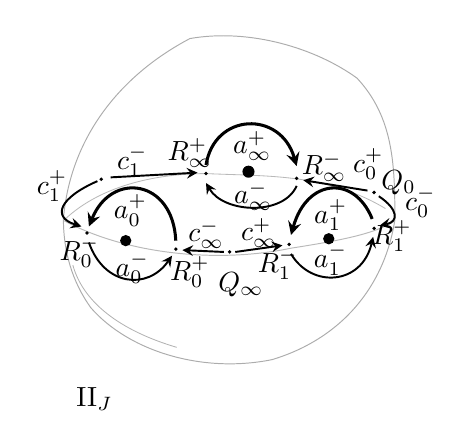
\begin{tikzpicture}[x=.012cm,y=-.012cm,>=stealth]
\draw[gray!65,line width=.35pt] (103,274)
 .. controls (110,190) and (161,123) .. (237,83)
 .. controls (300,72) and (370,93) .. (414,125)
 .. controls (453,167) and (454,218) .. (454,275)
 .. controls (443,346) and (397,401) .. (324,423)
 .. controls (250,438) and (172,414) .. (132,368)
 .. controls (112,340) and (103,308) .. (103,274);
\draw[gray!55,line width=.3pt] (104,275)
 .. controls (145,236) and (208,226) .. (254,226)
 .. controls (322,229) and (382,226) .. (444,263);
\draw[gray!55,line width=.35pt] (104,276)
 .. controls (171,312) and (268,321) .. (344,305)
 .. controls (395,297) and (433,290) .. (454,276);
\draw[gray!60,line width=.3pt] (113,323)
 .. controls (125,366) and (169,394) .. (223,410);
\coordinate (A) at (254,226); \coordinate (B) at (350,231);
\coordinate (C) at (128,289); \coordinate (D) at (222,306);
\coordinate (E) at (342,301); \coordinate (F) at (432,284);
\coordinate (U) at (143,232); \coordinate (V) at (432,246);
\coordinate (W) at (279,309);
\foreach \p in {A,B,C,D,E,F,U,V,W}{\fill (\p) circle (2.0);}
\fill (299,224) circle (6.4);
\fill (169,297) circle (6.0);
\fill (384,295) circle (6.0);
\draw[->,line width=1.1pt] (254,217)
 .. controls (263,161) and (333,159) .. (350,218);
\draw[->,line width=.7pt] (350,239)
 .. controls (336,271) and (273,268) .. (254,236);
\draw[->,line width=1.1pt] (222,297)
 .. controls (219,232) and (154,223) .. (130,282);
\draw[->,line width=.7pt] (130,299)
 .. controls (146,345) and (192,350) .. (218,313);
\draw[->,line width=1.1pt] (430,274)
 .. controls (411,227) and (361,231) .. (344,291);
\draw[->,line width=.7pt] (344,311)
 .. controls (366,348) and (419,344) .. (431,293);
\draw[->,line width=.7pt] (139,234)
 .. controls (98,252) and (91,272) .. (122,282);
\draw[->,line width=.7pt] (153,230)--(245,225);
\draw[->,line width=.7pt] (425,244)--(357,233);
\draw[->,line width=.7pt] (437,250)
 .. controls (458,264) and (458,277) .. (438,281);
\draw[->,line width=.7pt] (273,309)--(229,307);
\draw[->,line width=.7pt] (285,309)--(335,302);
\node at (303,197) {$a_\infty^+$};
\node at (304,250) {$a_\infty^-$};
\node at (174,265) {$a_0^+$};
\node at (176,326) {$a_0^-$};
\node at (386,270) {$a_1^+$};
\node at (386,317) {$a_1^-$};
\node at (91,239) {$c_1^+$};
\node at (176,213) {$c_1^-$};
\node at (426,216) {$c_0^+$};
\node at (481,256) {$c_0^-$};
\node at (254,290) {$c_\infty^-$};
\node at (310,289) {$c_\infty^+$};
\node at (237,204) {$R_\infty^+$};
\node at (379,219) {$R_\infty^-$};
\node at (120,309) {$R_0^-$};
\node at (237,330) {$R_0^+$};
\node at (330,322) {$R_1^-$};
\node at (451,292) {$R_1^+$};
\node at (458,236) {$Q_0$};
\node at (291,344) {$Q_\infty$};
\node at (136,465) {$\mathrm{II}_J$};
\end{tikzpicture}
}
On rajoute les sommets $Q_i$ $(i\in J)$ et les arcs
\diagram{\begin{tikzcd}[ampersand replacement=\&]Q_i\arrow[r,"c_i^\omega"]\&R_{\omega'i}^{\omega'}\end{tikzcd}}
permutés \inserted{de façon \unsure{simple|simplement}}
\unsure{transitive}\deleted{\unsure{ment}} par $G_J$. On a maintenant
\[
(13)\qquad b_i^\omega=c_i^\omega(c_i^{\omega'})^{-1}
\]
(donc les $b_i^\omega$ deviennent inutiles comme générateurs d'un groupoïde).
\inserted{Dans} Les relations \inserted{$(2)$} \deleted{deviennent},
la partie $(a)$ devient automatique, pour écrire commodément la partie $(b)$,
on introduit les
\[
(14)\qquad\widetilde a_i^\omega=
\begin{gathered}
(\unsure{c}_{\unsure{\omega i|\omega'i}}^{\omega\deleted{\unsure{'}}})^{-1}
a_i^{\omega\deleted{\unsure{'}}}
\unsure{c}_{\unsure{\omega'i|\omega i}}^{\omega'}\\[-2pt]
\inserted{(c_{\omega i}^\omega)^{-1}a_i^\omega c_{\omega'i}^{\omega'}}
\end{gathered}
:\quad Q_{\omega'i}\longrightarrow Q_{\omega i}
\]
\figure{
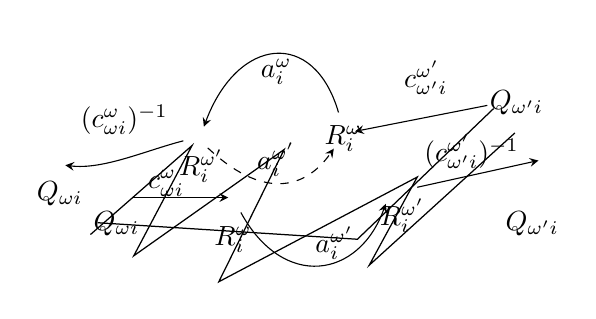
\begin{tikzpicture}[x=1cm,y=1cm,>=stealth]
\node (qu) at (0,0) {$Q_{\omega i}$};
\node (rl) at (1.8,.35) {$\unsure{R_i^{\omega'}}$};
\node (rr) at (3.6,.7) {$R_i^\omega$};
\node (qr) at (5.8,1.15) {$Q_{\omega'i}$};
\draw[->] (1.57,.67) .. controls (1.1,.55) and (.55,.3) .. (.07,.36);
\node at (.82,.94) {$(c_{\omega i}^\omega)^{-1}$};
\draw[->] (5.43,1.12)--(3.75,.79);
\node at (4.65,1.47) {$c_{\omega'i}^{\omega'}$};
\draw[->] (3.54,1.03) .. controls (3.23,2.1) and (2.26,2.0) .. (1.83,.85);
\node at (2.75,1.55) {$a_i^\omega$};
\draw[->,dashed] (1.88,.58) .. controls (2.56,-.06) and (3.1,.03) .. (3.48,.57);
\node at (2.75,.43) {$a_i^{\omega'}$};
\node at (.72,-.38) {$\deleted{\unsure{Q_{\omega i}}}$};
\node at (2.2,-.58) {$\deleted{\unsure{R_i^\omega}}$};
\node at (4.35,-.28) {$\deleted{\unsure{R_i^{\omega'}}}$};
\node at (6.0,-.38) {$\deleted{\unsure{Q_{\omega'i}}}$};
\draw[->] (.92,-.05)--(2.14,-.05);
\node at (1.35,.13) {$\deleted{\unsure{c_{\omega i}^\omega}}$};
\draw[->] (2.3,-.24) .. controls (2.84,-1.23) and (3.8,-1.08) .. (4.14,-.13);
\node at (3.49,-.63) {$\deleted{\unsure{a_i^{\omega'}}}$};
\draw[->] (4.54,.08)--(6.08,.42);
\node at (5.23,.53) {$\deleted{(c_{\omega'i}^{\omega'})^{-1}}$};
\draw[line width=.45pt] (.39,-.52)--(1.68,.61)--(.94,-.79)--(2.85,.56)
 --(2.02,-1.12)--(4.54,.21)--(3.93,-.91)--(5.78,.77);
\draw[line width=.45pt] (.48,-.37)--(3.78,-.58)--(5.51,1.08);
\end{tikzpicture}}
\margin{\figure{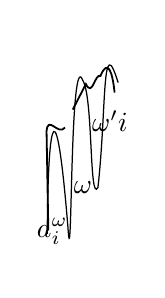
\begin{tikzpicture}[x=.45cm,y=.6cm]
\draw[line width=.45pt] (.05,.15) .. controls (.07,2.8) and (.32,3.28) .. (.65,.13)
 .. controls (.75,-.6) and (.7,4.1) .. (1.05,3.4)
 .. controls (1.35,3.05) and (1.23,.78) .. (1.48,1.13)
 .. controls (1.73,2.8) and (1.58,4.5) .. (2.05,3.35);
\draw[line width=.65pt] (.08,.22)--(.03,2.32)
 .. controls (.07,2.68) and (.36,2.21) .. (.55,2.4);
\draw[line width=.65pt] (.77,2.78)--(1.14,3.32)
 .. controls (1.33,3.03) and (1.39,3.55) .. (1.55,3.49)
 .. controls (1.76,3.87) and (1.89,3.58) .. (1.95,3.14);
\node at(.19,.2){$\unsure{a_i^\omega}$};
\node at(1.06,1.13){$\unsure{\omega}$};
\node at(1.82,2.53){$\unsure{\omega'i}$};
\end{tikzpicture}}}
qui sont également permutés de façon simpl. transitive sous $G_J$, et on a
\[
(15)\qquad\tau(\widetilde a_i^\omega)=(\widetilde a_i^{\omega'})^{-1}
\]
La relation $(2b)$ devient
\[
(16)\qquad\widetilde a_{\omega^2i}^\omega\widetilde a_{\omega i}^\omega\widetilde a_i^\omega=1
\]
(deux relations ess\textsuperscript{t}. distinctes\unsure{,} qui sont permutées par $\tau$)

Pour repérer les \inserted{$\pi(Q_{\unsure{J|i}})=$}
$\pi_1(\Sigma_J(\mathbb C),Q_i)$ de façon commode on utilise les
\diagram{
\begin{tikzcd}[ampersand replacement=\&,column sep=large,row sep=large]
(17)\quad\psi_i^\omega:\ \deleted{Q_i}\Pi_{0,3}
\arrow[rr,"\sim"]
\arrow[dr,"\varphi_{\omega'i}^{\omega'}","\sim"',sloped]
\&\&\pi(Q_i)\\
\&\pi(R_{\omega'i}^{\omega'})
\arrow[ur,"(c_i^\omega)^{-1}"',"\sim",sloped]
\arrow[ur,phantom,near end,"\deleted{\unsure{c|\sim}}"]\&
\end{tikzcd}}
\margin{\uline{NB}\quad$\tau\psi_i^\omega(g)=\psi_i^\omega(\tau_\infty g)$}
on aura
\[
(18)\qquad\psi_i^\omega(g)=\psi_i^{\omega'}(\sigma_\infty(g))
\]
\[
(19)\qquad\begin{aligned}
\widetilde a_i^{\omega\deleted{\unsure{'|*}}}
(\psi_{\omega'i}^{\omega'}(g))
&=\psi_{\omega\deleted{\unsure{'}}i}^{\omega\deleted{\unsure{'}}}
(\varepsilon_0(g))
=\psi_{\omega\deleted{\unsure{'}}i}^{\omega'}
(\overbrace{\sigma_\infty\varepsilon_0}^{\deleted{\unsure{\xi|\rho}}=\tau_\infty(\rho)}(g))
\end{aligned}
\]
\[
\begin{array}{|c|}\hline
\displaystyle \widetilde a_i^\omega(\psi_{\omega'i}^{\omega}(g))
=\psi_{\omega\deleted{\unsure{'}}i}^{\omega\deleted{\unsure{'}}}
(\overbrace{\varepsilon_0\deleted{\unsure{(}}\sigma_\infty}^{\rho^{-1}})(g))\\
\end{array}
=\psi_{\omega'i}^{\omega'}(\sigma_\infty\varepsilon_0\sigma_\infty(g))
\]
\margin{25}

\scanpage{27}
\mspage{8}
On prend un autom. \inserted{$u$} des groupoïdes $\widehat{\mathrm{II}}_J$ qui \inserted{commute à $G_J$ et qui} fixe les sommets, et qui comme plus haut laisse stables les sous-groupoïdes $\widehat{\mathrm{II}}_{J,i}$ $(i\in J)$, \deleted{\unsure{les groupoïdes}} $\mathrm{II}_{J,i}$ engendré par les \inserted{2} sommets $R_i^\omega$ $(\omega\in\uline{\omega})$ et les deux flèches $a_i^\omega$ $(\omega\in\uline{\omega})$.
\deleted{\unsure{Alors}} L'endom. $u$ est connu quand on connaît les $u(a_i^\omega)$, qui sont de la forme
\[
(20)\qquad u(a_i^\omega)=a_i^\omega\varphi_i^\omega\bigl(\underbrace{l_0^\gamma}\bigr)
\qquad\begin{array}{l}\gamma\unsure{\ne|=}\frac{p-1}{2}\in\widehat{\mathbb Z}\\p\in\widehat{\mathbb Z}^{*}\end{array}
\]
\margin{NB: $\lambda\in\widehat\Pi_{0,3}$, pas la peine d'exiger de prime abord que $\lambda$ de la forme $l_0^\gamma\ldots$}
\uline{et} les
\[
(21)\qquad u(c_i^\omega)=\varphi_{\omega'i}^{\omega'}(\eta)c_i^\omega=c_i^\omega\psi_i^\omega(\eta)
\qquad\eta\in\widehat\Pi_{0,3}\quad\text{indépendant de }i,\omega
\]
On aura alors (comparer $(11)$)
\[
(22)\qquad u(b_i^\omega)=b_i^\omega\varphi_{\omega i}^\omega(\beta)\qquad\text{avec}
\]
\[
(23)\qquad\beta=\sigma_\infty(\eta)\eta^{-1}
\]
\margin{NB devient plus joli si $\eta$ est remplacé par son $\sigma_\infty(\eta)$, ou $\beta$ par $\beta^{-1}$}
Les relations à satisfaire sont alors déjà écrites en \inserted{$p$ (ou $\gamma$) et} $\beta$, \deleted{\unsure{la}} dans $(12)$ --- mais la première relation $\beta\sigma_\infty(\beta)=1$ conséquence de $(23)$, il reste la deuxième qui s'écrit donc
\margin{\uline{NB} Si $u$ remplacé par $u'=\tau(u)$, alors $\eta$ est remplacé par $\eta'=\tau_\infty(\eta)$, $\beta$ par $\tau_\infty(\beta)$, mais $\lambda$ par $\varepsilon_0^{-1}(\tau_\infty(\lambda^{-1}))$}
\[
(24)\qquad\deleted{\unsure{(l_1^{-\gamma}\sigma_\infty(\eta)\eta^{-1}}}
\quad\alpha\rho^{-1}(\alpha)\rho^{-\unsure{2|1}}(\alpha)=1
\qquad\text{avec}\quad\alpha=\underbrace{l_1^\gamma}_{\sigma_\infty(\lambda)}\underbrace{\sigma_\infty(\eta)\eta^{-1}}_\beta.
\]
On aura ici
\[
(25)\qquad
u(\widetilde a_i^\omega)=\psi_{\omega\unsure{\deleted{'}|^{*}}i}^{\omega\unsure{\deleted{'}|^{*}}}\bigl(\underbrace{\eta^{-1}l_0^\gamma\varepsilon_0(\eta)}_{\widetilde\alpha=\eta^{-1}\varepsilon_0(\lambda\eta)}\bigr)\widetilde a_i^\omega
=\widetilde a_i^\omega\psi_{\omega'i}^{\omega'}\bigl(\underbrace{\varepsilon_0^{-1}(\eta^{-1})l_0^\gamma\eta}_{\varepsilon_0^{-1}(\widetilde\alpha)}\bigr)
\]
\inserted{, valable quel que soit $\lambda$}
\margin{$\widetilde\alpha=\eta^{-1}l_0^\gamma\varepsilon_0(\eta)$}
et
\[
(25\text{ bis})\quad\deleted{\alpha=}\quad\alpha=\rho\bigl(\eta\widetilde\alpha\rho^{-1}(\eta)^{-1}\bigr)
\]
\margin{valable pour $\lambda$ quelconque, pas \unsure{néc|néc.} de la forme $l_0^\gamma$.}
\deleted{\unsure{car}} dans l'équation $(24)$ en $\alpha$ (invariante par substitutions $\alpha\mapsto\rho^{-1}(\alpha)$ (ou $\alpha\mapsto\rho\alpha=\rho^{-2}(\alpha)$) et $\alpha\mapsto x\alpha\rho^{-1}(x)^{-1}$,
\margin{26}

\scanpage{28}
\mspage{9}
équivaut à l'équation \deleted{\unsure{identique}} \deleted{\unsure{correspondante}} \inserted{analogue} en $\widetilde\alpha$
\[
(26)\qquad\widetilde\alpha\rho^{-1}(\widetilde\alpha)\rho^{\unsure{-2}}(\unsure{\widetilde\alpha|\widehat\alpha})=1,
\qquad\boxed{(27)\quad\widetilde\alpha=\eta^{-1}l_0^\gamma\varepsilon_0(\eta)}
\]
\deleted{$\unsure{\varepsilon}$}

Considérons maintenant le groupoïde \inserted{$\mathrm{III}_J$} induit par le groupoïde précédent \inserted{$\mathrm{II}_J$} sur l'ens des trois sommets $Q_i$, c'est aussi le groupoïde engendré par le graphe à trois sommets $Q_i$ $(i\in J)$ et six arcs orientés $\widetilde a_i^\omega$ et leurs opposés, avec les seules relations $(16)$ (ens de 6 relations stable par $G_J$, et se réduisant en fait à deux relations effectives\ldots).

\figure{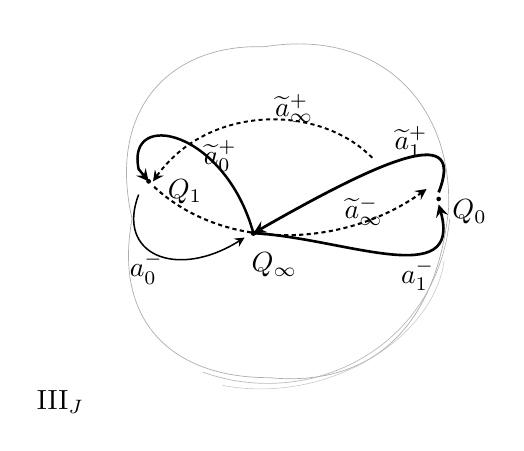
\begin{tikzpicture}[x=.014cm,y=-.014cm,>=stealth]
\draw[gray!65,line width=.25pt] (48,173) .. controls (25,73) and (83,14) .. (168,17)
 .. controls (272,0) and (338,68) .. (335,163)
 .. controls (326,259) and (275,327) .. (172,317)
 .. controls (82,317) and (31,264) .. (48,173);
\draw[gray!55,line width=.25pt] (112,312) .. controls (210,347) and (324,290) .. (336,173);
\draw[gray!45,line width=.2pt] (130,324) .. controls (225,342) and (321,282) .. (331,211);
\coordinate (A) at (63,139);
\coordinate (B) at (158,186);
\coordinate (C) at (326,155);
\fill (A) circle (2.2);\fill (B) circle (2.5);\fill (C) circle (2.1);
\draw[->,line width=.9pt] (B) .. controls (132,92) and (42,73) .. (54,128) -- (A);
\draw[->,line width=.55pt] (54,151) .. controls (33,205) and (88,229) .. (150,190);
\draw[->,line width=1pt] (326,149) .. controls (350,88) and (282,115) .. (B);
\draw[->,line width=.95pt] (B) .. controls (238,190) and (348,239) .. (326,160);
\draw[<-,line width=.7pt,dash pattern=on 1.5pt off 1.2pt] (67,139)
 .. controls (117,69) and (219,68) .. (267,119);
\draw[->,line width=.75pt,dash pattern=on 1.5pt off 1.2pt] (68,144)
 .. controls (133,204) and (241,199) .. (315,146);
\node at (96,148) {$Q_1$};
\node at (177,215) {$Q_\infty$};
\node at (354,167) {$Q_0$};
\node at (128,116) {$\widetilde a_0^+$};
\node at (61,218) {$a_0^-$};
\node at (301,103) {$\widetilde a_1^+$};
\node at (307,224) {$a_1^-$};
\node at (195,73) {$\widetilde a_\infty^+$};
\node at (258,166) {$\widetilde a_\infty^-$};
\node at (-17,339) {$\mathrm{III}_J$};
\end{tikzpicture}}

Le groupe $\{1,\tau\}$ y opère dans le graphe avec relations, par
\[
(27)\qquad\tau Q_i=Q_i,\quad\tau\widetilde a_i^\omega=(\widetilde a_i^{\omega'})^{-1}
\]
La donnée d'un \deleted{\unsure{autom.}} \inserted{endom.} du groupoïde $\widehat{\mathrm{III}}_J$, fixant les sommets et commutant à $G_J$, équivaut à celle d'un $\widetilde\alpha\in\widehat\Pi_{0,3}$, \deleted{$\unsure{\gamma|\lambda}\in\widehat{\mathbb Z}$}, satisfaisant \deleted{\unsure{l'équation rel.}} $(26)$. On aura, en introduisant
\[
(28)\qquad\widetilde\lambda_i^\omega=\widetilde a_i^{\omega'}\widetilde a_i^\omega,\in\deleted{\unsure{Q_{\omega'i}}}\inserted{\pi(Q_{\omega'i})}
\]
(\unsure{comparer à la définition dans le groupoïde} $\mathrm{II}_J$ ! $\lambda_i^\omega=\overset{\unsure{\deleted{\sim}|\sim}}{a}_i^{\omega'}a_i^\omega$)

\figure{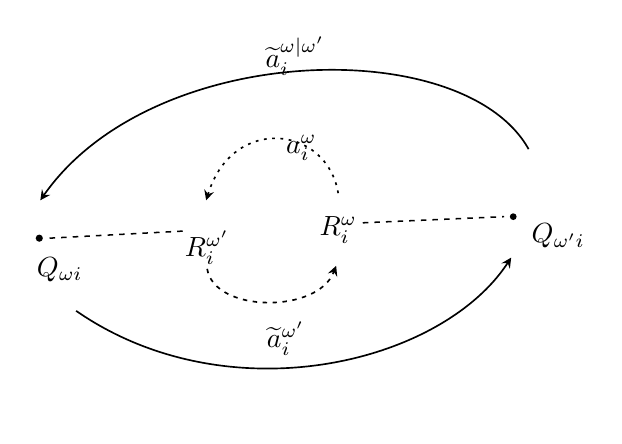
\begin{tikzpicture}[x=.013cm,y=-.013cm,>=stealth]
\fill (22,194) circle (3.5);
\fill (485,173) circle (3.3);
\draw[->,line width=.6pt] (500,107) .. controls (437,-6) and (132,1) .. (23,157);
\draw[->,line width=.6pt] (58,265) .. controls (205,367) and (414,318) .. (483,213);
\draw[line width=.55pt,dash pattern=on 2pt off 2.2pt] (32,194) -- (164,187);
\draw[line width=.55pt,dash pattern=on 2pt off 2.2pt] (338,179) -- (476,173);
\draw[->,line width=.6pt,dash pattern=on 1pt off 2pt] (314,150)
 .. controls (303,84) and (211,73) .. (185,157);
\draw[->,line width=.6pt,dash pattern=on 1.6pt off 2pt] (186,224)
 .. controls (193,267) and (294,268) .. (312,221);
\node at (42,225) {$Q_{\omega i}$};
\node at (529,192) {$Q_{\omega'i}$};
\node at (186,203) {$R_i^{\omega'}$};
\node at (314,186) {$R_i^\omega$};
\node at (272,16) {$\widetilde a_i^{\unsure{\omega|\omega'}}$};
\node at (263,292) {$\widetilde a_i^{\omega'}$};
\node at (278,106) {$a_i^\omega$};
\end{tikzpicture}}

\margin{\deleted{il semblerait raisonnable de changer les notations $\widetilde a_i^\omega$ devenant $\widetilde a_i^{\omega'}$}\quad $*$ \unsure{obtenir}, \unsure{une définition des} $\psi_i^\alpha$ \unsure{qui} \unsure{donne} dans $(29)$ \unsure{ainsi}. \unsure{cf.} \unsure{voir} \unsure{plus bas}}
\[
(29)\qquad u(\widetilde\lambda_i^\omega)=\overset{*}{\psi_{\omega'i}^{\omega'}}(\widetilde\alpha\varepsilon_0(\widetilde\alpha))\widetilde\lambda_i^\omega
=\psi_{\omega'i}^{\omega'}(\widetilde\alpha\varepsilon_0(\widetilde\alpha)l_0)
\]
Dans le cas où $\widetilde\alpha$ provient de $\eta,\gamma$ par $(27)$, on aura
\[
(30)\qquad\widetilde\alpha\varepsilon_0(\widetilde\alpha)l_0=\eta^{-1}l_0^p\eta\qquad(p=2\gamma+1)\ ;
\]
\margin{27}

\scanpage{29}
\mspage{(10)}
\margin{\uline{NB} Ce sous-groupoïde $\mathrm{III}_{J,i}$ (de groupe fondamental $\widehat{\mathbb Z}$) engendré par les sommets $Q_j$ $(j\in J\setminus\{i\})$ et les deux $\unsure{\widetilde a_i^\omega|\text{arêtes}}$ \unsure{orientés} qui les joignent, \uuline{n'est \deleted{\unsure{donc}} pas} stable \uline{par $u$} !}
en d'autres termes faisons opérer $u$ sur $\pi(Q_{\omega'i})$, identifié à $\widehat\Pi_{0,3}$ via $\psi_{\omega'i}^{\omega'}$, $\widetilde\lambda_i^\omega$ identifié à $l_0$, on trouve que $u(l_0)$ est conjugué de $l_0^p$, \deleted{\unsure{avec}} la conjugaison étant effectuée par $\eta^{-1}$ (par la formule $(30)$).

Le passage de $u$ à $\tau(u)$ s'exprime par
\deleted{\unsure{J'en prends} maintenant les points $P_\omega^{\unsure{\omega}}$ $(\omega\in\uline{\omega})$}
le passage de $\widetilde\alpha$ à
\[
(31)\qquad\widetilde\alpha'=\varepsilon_0\tau_\infty(\widetilde\alpha^{-1})
={\underbrace{\rho^{-1}\underline{\widetilde\sigma_\infty\vphantom{(\widetilde\alpha^{-1})}}}_{\widetilde\sigma_0}}\underline{(\widetilde\alpha^{-1})\vphantom{\widetilde\sigma_\infty}}
\]
\margin{où $\widetilde\sigma_\infty=\sigma_\infty\tau_\infty=\tau_\infty\sigma_\infty$ est dans l'image de l'hom canonique
\diagram{\begin{tikzcd}[ampersand replacement=\&]
\unsure{\widetilde G_3|G_3}\arrow[r]\arrow[d,phantom,"\simeq"{rotate=90,description}] \& \widetilde\Pi_{0,3}\\
\deleted{\text{\unsure{du}}\ \unsure{\widetilde G_3|G_3}} \&
\end{tikzcd}}
stabilisateur de $P_+$ dans $G_3\times\{1,\tau\}$}
\[
\widetilde\sigma_i(l_i)=l_i^{-1}
\]
\[
\widetilde\sigma_i(l_j)=l_k^{-1}\quad\text{si }\{0,1,\infty\}=\{i,j,k\}
\]
\uline{NB} Le groupe $\widetilde G_3$ opère sur $\Pi_{0,3}$ et contient \deleted{$\unsure{\xi_3|\widetilde G_3}$} \deleted{\unsure{dont il}} $\{1,\rho^{-1},\rho^{-2}_{\unsure{\prime\prime|\mathrm{II}}}\}$ comme ss-groupe \inserted{$\widetilde G_3^+$} d'indice 2, \deleted{\unsure{et|dont} $\widetilde G_3$ \unsure{conjugue} $\rho$} $\widetilde G_3/\widetilde G_3^+$ opère sur $\widetilde G_3^+$ en échangeant $\rho$ et $\rho^{-1}$, il s'ensuit que $\widetilde G_3$ opère sur $V$ ens des solutions $x$ de l'équation
\[
x\rho^{-1}(x)\rho^{-2}(x)=1
\]
par
\[
(32)\qquad\Theta_g x=g.x^{\operatorname{sg}(g)}
\]
et on a ici
\[
(33)\qquad\widetilde\alpha'=\Theta_{\widetilde\sigma_0}(\widetilde\alpha)
\]
\margin{28}

\scanpage{30}
\margin{29}
\mspage{11}
\margin{\uline{NB} les flèches $\widetilde a_i^\omega$ sont en fait superflues, cf $(37)$ et commentaires p. 19.}
\figure{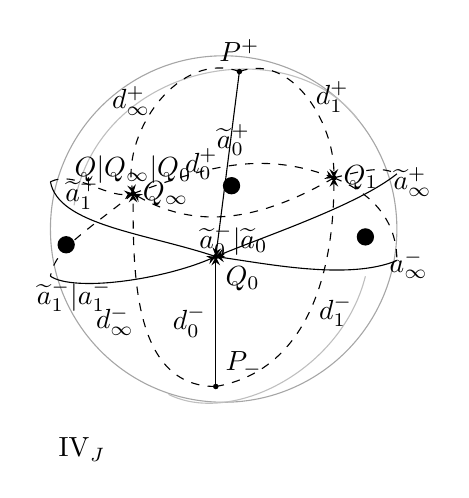
\begin{tikzpicture}[x=1cm,y=1cm,>=stealth]
\draw[gray!70] (0,0) ellipse (2.2 and 2.2);
\draw[gray!50] (-1.9,.3) .. controls (-1.6,2.1) and (.8,2.55) .. (1.7,1.4);
\draw[gray!50] (-.7,-2.1) .. controls (.1,-2.5) and (1.5,-1.8) .. (1.8,-.6);
\coordinate(P) at(.2,2);\coordinate(M) at(-.1,-2);\coordinate(A) at(-1.15,.45);\coordinate(B) at(1.4,.65);\coordinate(C) at(-.1,-.35);
\foreach \p in {P,M,A,B,C}{\fill (\p) circle(.035);}
\fill (-2,-.2) circle(.11);\fill(.1,.55) circle(.11);\fill(1.8,-.1) circle(.11);
\draw[->,dashed] (P) to[out=160,in=100] node[left]{$d_\infty^+$}(A);
\draw[->] (P)--node[left]{$d_0^+$}(C);
\draw[->,dashed] (P) to[out=20,in=90] node[right]{$d_1^+$}(B);
\draw[->,dashed] (M) to[out=180,in=270] node[left]{$d_\infty^-$}(A);
\draw[->] (M)--node[left]{$d_0^-$}(C);
\draw[->,dashed] (M) to[out=10,in=270] node[right]{$d_1^-$}(B);
\draw[->,dashed] (A) to[out=20,in=160] node[above]{$\widetilde a_0^+$}(B);
\draw[->,dashed] (B) to[out=210,in=330] node[below]{$\unsure{\widetilde a_0^-|\widetilde a_0}$}(A);
\draw (C) .. controls (-1.0,-.05) and (-2.1,.05) .. (-2.2,.6);
\draw[->,dashed] (-2.2,.6) .. controls (-1.9,.75) and (-1.5,.4) .. (A);
\node at(-1.8,.45){$\widetilde a_1^+$};
\draw[dashed] (A) .. controls (-1.7,.0) and (-2.15,-.25) .. (-2.2,-.6);
\draw[->] (-2.2,-.6) .. controls (-1.9,-.8) and (-.8,-.65) .. (C);
\node at(-1.9,-.85){$\unsure{\widetilde a_1^-|a_1^-}$};
\draw[dashed] (B) .. controls (1.8,.75) and (2.0,.8) .. (2.2,.7);
\draw[->] (2.2,.7) .. controls (1.7,.3) and (.5,-.1) .. (C);
\node at(2.4,.6){$\widetilde a_\infty^+$};
\draw[dashed] (B) .. controls (1.9,.45) and (2.2,.1) .. (2.2,-.4);
\draw[->] (2.2,-.4) .. controls (1.6,-.65) and (.6,-.45) .. (C);
\node at(2.35,-.45){$a_\infty^-$};
\node[above] at(P){$P^+$};\node[above right] at(M){$P_-$};
\node[right] at(A){$Q_\infty$};\node[right] at(B){$Q_1$};\node[below right] at(C){$Q_0$};
\node[above] at(A){$\deleted{\unsure{Q|Q_\infty|Q_0}}$};\node at(-1.8,-2.8){$\mathrm{IV}_J$};
\end{tikzpicture}}
On rajoute les \inserted{deux} sommets $\unsure{P_i^\omega|P_\infty^\omega}$ $(\omega\in\uline{\omega})$, et les flèches
\diagram{\begin{tikzcd}[ampersand replacement=\&]d_i^\omega:\quad P_\infty^\omega\arrow[r]\&Q_i\end{tikzcd}}
permutés transitivement par $G_J$, avec
\[
(34)\qquad\tau(P_{\unsure{\infty|i}}^\omega)=P_{\unsure{\infty|i}}^{\omega'},\qquad\tau(d_i^\omega)=d_i^{\omega'}
\]
Le groupoïde $\mathrm{III}_J$ est équivalent au groupoïde $\mathrm{IV}_J$ \inserted{défini par le graphe ayant} \deleted{\unsure{sur}} les sommets $Q_i$ $(i\in\omega)$ et $P_\infty^\omega$ $(\omega\in\uline{\omega})$, les arcs $\widetilde a_i^\omega$ et $d_i^\omega$ et les \inserted{arcs} opposés, et les six relations
\[
(35)\qquad(d_{\omega'i}^\omega)^{-1}\widetilde a_{\omega i}^{\omega}d_i^\omega=1
\]
(qui impliquent d'ailleurs les relations constitutives $(16)$ pour $\mathrm{III}_J$). La donnée d'un endomorphisme de $\mathrm{IV}_J$ qui fixe les \deleted{pts} sommets (pour simplifier --- il faudra regarder aussi ceux qui permutent les sommets \inserted{$P_\omega$}, en fixant les $Q_i$), \deleted{équivaut à} et qui commute à $G_J$, équivaut à la donnée des
\[
(36)\quad\left\{\begin{aligned}
u(\widetilde a_i^\omega)&=\psi_{\omega i}^\omega(\widetilde\alpha)\widetilde a_i^\omega
&\widetilde\alpha&\in\widehat\Pi_{03}\quad\text{(indép. de }i,\omega\text{)}\\
u\bigl(\overset{\deleted{\unsure{u|\omega}}}{d_i^\omega}\bigr)&=\psi_i^\omega(\xi)d_i^\omega\quad\bigl(=d_i^\omega\widetilde\psi_i^\omega(\xi)\bigr)
&\xi&\in\widehat\Pi_{0,3}\quad\cdot\,\cdot\,\cdot\,\cdot\,\cdot
\end{aligned}\right.
\]
de $\widetilde\alpha,\xi\in\widehat\Pi_{0,3}$, avec la relation déduite de $(35)$, on trouve \unsure{les|\deleted{les}} équations
\[
(37)\qquad\widetilde\alpha=\xi.\rho^{-1}(\xi^{-1})
\]
i.e. $\widetilde\alpha$ est connu quand on connait $\xi\in\widehat\Pi_{0,3}$
\margin{il n'y a donc pas de \unsure{condition|conditions} sur $\xi$ ici.}

\scanpage{31}
\mspage{(12)}
qui implique bien sûr (26).

\margin{revenant avant l'introduction de $u$}
\margin{\uline{NB} le passage de $u$ à $\tau(u)$ s'exprime par
$\xi\mapsto\sigma_\infty\tau_\infty(\xi)=\widetilde\sigma_\infty(\unsure{\xi})$}
Je \deleted{vais} considère les isomorphismes
\diagram{$(38)\qquad$
\begin{tikzcd}[ampersand replacement=\&,column sep=large,row sep=large]
\Pi_{0,3}\arrow[rr,"\widetilde\psi_i^\omega"]\arrow[dr,"\psi_i^\omega"']\&\&\pi(P^\omega)\\
\&\pi(Q_i)\arrow[ur,"(d_{\unsure{i}}^\omega)^{-1}"']\&
\end{tikzcd}}
\margin{\deleted{\unsure{Changement} \unsure{de base} \unsure{défini} de l'iso $\Pi_{0,3}\simeq\Pi_{0,3}$} pour \unsure{une} \unsure{compatib.}}

de sorte que les relations (35) et (19) donnent
\[
(39)\qquad \widetilde\psi_{\omega i}^\omega(g)=\widetilde\psi_i^\omega\left(\overset{\text{\textcircled{$\scriptstyle\rho^{-1}?$}}}{\rho}g\right)
\qquad\text{i.e.}\quad\widetilde\psi_{\omega i}=\widetilde\psi_i\circ\rho,
\]
et j'introduis les chemins
\[
(40)\qquad\widetilde d_i^\omega:
\begin{tikzcd}[ampersand replacement=\&,column sep=large]
P_\xi^\omega\arrow[r,no head]\&P_\xi^{\omega'}
\end{tikzcd},\qquad
\widetilde d_i^\omega=(d_i^{\omega'})^{-1}d_i^\omega
\]
permutés de façon simplement transitive par $G_J$,
\deleted{de \illegible{1} et satisfaisant} satisfaisant
\[
(\unsure{41|=41})\qquad\tau(\unsure{\widetilde d_i^\omega|d_i^\omega})=\widetilde d_i^{\omega'},\qquad
d_i^\omega d_i^{\omega'}=1
\]
On \deleted{\unsure{aura donc}} \inserted{a} les relations
\[
(42)\qquad\widetilde d_i^\omega(\widetilde\psi_i^\omega(g))=
\widetilde\psi_i^{\omega'}(\sigma_\infty(g)).
\]
Revenant à l'\deleted{auto}morphisme $u$, on aura \deleted{\unsure{automatiquement}}
\[
(43)\qquad u(\widetilde d_i^\omega)=\widetilde\psi_i^{\omega'}(\unsure{\sigma_\infty}(\widetilde\beta))\widetilde d_i^\omega
=\widetilde d_i^\omega\widetilde\psi_i^\omega(\widetilde\beta)
\]
avec
\[
(44)\qquad\widetilde\beta=\xi\sigma_\infty(\xi)^{-1}:
\]
satisfaisant, \inserted{donc} \deleted{\unsure{ainsi}} comme $\widetilde\beta$ tantôt, la relation
\[
(45)\qquad\widetilde\beta\sigma_\infty(\widetilde\beta)=1
\]

Considérons maintenant \unsure{le|les} ss-\unsure{groupoïde|groupes} de
\margin{30}

\scanpage{33}
\mspage{14}
\figure{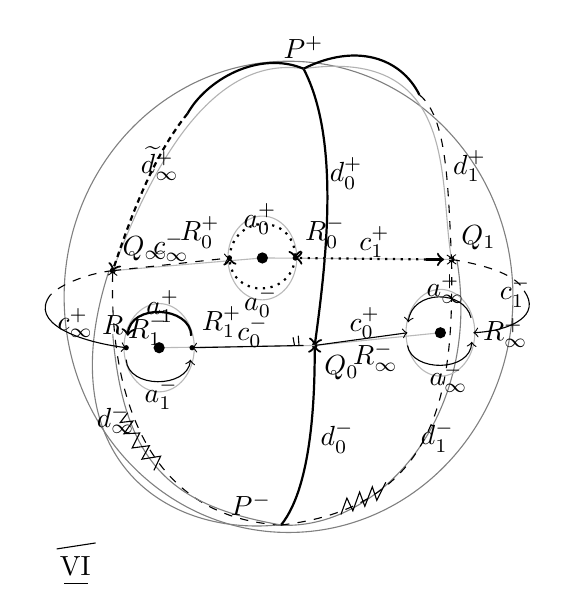
\begin{tikzpicture}[scale=.95]
\draw[gray] (0,0) ellipse (3 and 3.15);
\draw[gray] (-2.4,.35)..controls (-3.2,-2.1) and (-1.7,-3.2)..(-.15,-3.05);
\draw[gray] (2.25,.5)..controls (2.6,-1.6) and (1.2,-3.15)..(-.15,-3.05);
\coordinate (Pp) at (.2,3.05);\coordinate (Pm) at (-.1,-3.05);
\coordinate (Qi) at (-2.35,.35);\coordinate (Qz) at (.35,-.65);\coordinate (Qo) at (2.18,.5);
\draw[gray!60] (Pp)..controls (-1.1,3.25) and (-1.9,1.55)..(Qi);
\draw[thick] (Pp)..controls (-.4,3.3) and (-1.1,2.9)..(-1.35,2.45);
\draw[dash pattern=on 2pt off 1.5pt,->,thick] (-1.35,2.45)..controls (-1.8,1.9) and (-2.1,1.1)..(Qi);
\draw[->,thick] (Pp)..controls (.7,2.1) and (.5,.45)..(Qz);
\draw[gray!60] (Pp)..controls (2.3,3.35) and (2,1.5)..(Qo);
\draw[thick] (Pp)..controls (.9,3.4) and (1.5,3.2)..(1.75,2.7);
\draw[dashed,->] (1.75,2.7)..controls (2.12,2.4) and (2.13,1.5)..(Qo);
\draw[dashed,->] (Pm)..controls (-1.95,-2.95) and (-2.4,-1.2)..(Qi);
\draw[->,thick] (Pm)..controls (.35,-2.5) and (.35,-1.1)..(Qz);
\draw[dashed,->] (Pm)..controls (2.1,-2.8) and (2.2,-1.1)..(Qo);
\draw[gray] (-2.35,-.5)..controls (-2.2,-2.3) and (-1.5,-2.8)..(-.1,-3.05);
\draw (-2.15,-1.55)--(-2.25,-1.68)--(-2.08,-1.66)--(-2.2,-1.83)--(-1.99,-1.82)--(-2.09,-2.02)--(-1.86,-1.99)--(-1.96,-2.17)--(-1.71,-2.13)--(-1.8,-2.32);
\draw (.7,-2.91)--(.78,-2.69)--(.86,-2.86)--(.95,-2.61)--(1.02,-2.8)--(1.12,-2.54)--(1.18,-2.72)--(1.3,-2.48);
\foreach \p in {Qi,Qz,Qo}{\fill (\p) circle (.04);}
\node[above] at (Pp) {$P^+$};\node[above left] at (Pm) {$P^-$};
\node[above right] at (Qi) {$Q_\infty$};\node[below right] at (Qz) {$Q_0$};\node[above right] at (Qo) {$Q_1$};
\node at (-1.72,1.78) {$\widetilde d_\infty^+$};\node at (.77,1.65) {$d_0^+$};\node at (2.42,1.75) {$d_1^+$};
\node at (-2.31,-1.64) {$d_\infty^-$};\node at (.65,-1.88) {$d_0^-$};\node at (1.99,-1.87) {$d_1^-$};
\draw[gray!55] (-.35,.52) ellipse (.46 and .56);
\draw[gray!55] (-1.73,-.68) ellipse (.47 and .59);
\draw[gray!55] (2.03,-.48) ellipse (.46 and .58);
\draw[gray!55] (Qi)--(-.35,.52)--(Qo);
\draw[gray!55] (-1.73,-.68)--(Qz)--(2.03,-.48);
\fill (-.35,.52) circle (.075);\fill (-1.73,-.68) circle (.075);\fill (2.03,-.48) circle (.075);
\coordinate (Rzp) at (-.79,.52);\coordinate (Rzm) at (.09,.52);
\coordinate (Rom) at (-2.17,-.68);\coordinate (Rop) at (-1.29,-.68);
\coordinate (Rim) at (1.59,-.48);\coordinate (Rip) at (2.47,-.48);
\draw[dotted,thick,->] (Rzp)..controls (-.75,1.12) and (.07,1.12)..(Rzm);
\draw[dotted,thick,->] (Rzm)..controls (.03,-.02) and (-.75,-.02)..(Rzp);
\draw[->,thick] (-1.30,-.52)..controls (-1.31,-.12) and (-2.12,-.08)..(-2.15,-.52);
\draw[->] (-2.17,-.84)..controls (-2.15,-1.23) and (-1.35,-1.23)..(-1.31,-.84);
\draw[->] (2.44,-.28)..controls (2.35,.1) and (1.65,.1)..(1.60,-.34);
\draw[->] (1.59,-.65)..controls (1.65,-1.01) and (2.43,-1.01)..(2.45,-.60);
\foreach \p in {Rzp,Rzm,Rom,Rop}{\fill (\p) circle (.035);}
\node[above left] at (Rzp) {$R_0^+$};\node[above right] at (Rzm) {$R_0^-$};
\node[above right,inner sep=.5pt] at (Rom) {$R_1^-$};\node[above right] at (Rop) {$R_1^+$};
\node at (-2.35,-.38) {$\unsure{R}$};
\node[below left] at (Rim) {$R_\infty^-$};\node[right] at (Rip) {$R_\infty^+$};
\node at (-.38,1.04) {$a_0^+$};\node at (-.37,-.07) {$a_0^-$};
\node at (-1.68,-.13) {$a_1^+$};\node at (-1.7,-1.3) {$a_1^-$};
\node at (2.1,.11) {$a_\infty^+$};\node at (2.14,-1.08) {$a_\infty^-$};
\draw[dashed,->] (Qi)--(Rzp);\node at (-1.57,.67) {$c_\infty^-$};
\draw[dashed] (Qi)..controls (-2.65,.32) and (-3.03,.18)..(-3.18,.03);
\draw[->] (-3.18,.03)..controls (-3.48,-.35) and (-2.8,-.6)..(Rom);\node at (-2.85,-.35) {$c_\infty^+$};
\draw[dotted,thick,->] (1.84,.5)--(Rzm);
\draw[->,thick] (1.84,.5)--(2.08,.5);\node at (1.15,.73) {$c_1^+$};
\draw[dashed] (Qo)..controls (2.55,.44) and (3.04,.32)..(3.15,.08);
\draw[->] (3.15,.08)..controls (3.38,-.24) and (3,-.45)..(Rip);\node at (3.03,.07) {$c_1^-$};
\draw[->] (.20,-.65)--(Rop);
\draw (.08,-.65)--(.06,-.54);\draw (.14,-.65)--(.13,-.52);
\node at (-.48,-.47) {$c_0^-$};
\draw[->] (Qz)--(Rim);\node at (1.02,-.35) {$c_0^+$};
\node at (-2.85,-3.6) {$\mathrm{VI}$};
\draw (-3.10,-3.37)--(-2.58,-3.29);\draw (-3.00,-3.83)--(-2.68,-3.83);
\end{tikzpicture}}
C'est le groupoïde engendré par ces sommets, les arêtes $a_i^\omega,c_i^\omega,d_i^\omega$ (trois paquets, \deleted{\unsure{permutés}} \inserted{ch. un} un torseur sous $G_J$) et les \inserted{six} relations
\[
(48)\qquad(d_{\omega i}^\omega)^{-1}(c_{\omega i}^{\omega'})^{-1}(a_{\unsure{\omega'i|\omega i}}^\omega)^{-1}c_i^\omega d_i^\omega=1
\]
\deleted{\unsure{Hom.}} L'automorphisme $\tau$ est donné par
\[
(49)\qquad\left\{\begin{aligned}
\tau(R_i^\omega)&=R_i^\omega,&\tau Q_i&=Q_i,&\tau(P_{\deleted{\unsure{\infty}}}^\omega)&=P^{\omega'}\\
\tau(a_i^\omega)&=(a_i^{\omega'})^{-1},&\tau(c_i^\omega)&=\unsure{c_i^\omega)|c_i^{\omega'}}&\tau(d_i^\omega)&=d_i^{\omega'}
\end{aligned}\right.
\]
Les $\pi_1\unsure{\varepsilon}$ de les sommets $R_i^\omega,Q_i,P^\omega$ sont repérés respectivement, en termes de $\Pi_{03}$, par ces isomorphismes
\[
(50)\qquad\left\{\begin{gathered}
\begin{tikzcd}[ampersand replacement=\&,column sep=large]
\Pi_{03}\arrow[r,"\varphi_i^\omega"]\&\pi(R_i^\omega)\deleted{\longrightarrow\pi(}
\end{tikzcd}\\
\begin{tikzcd}[ampersand replacement=\&,column sep=large]
\Pi_{03}\arrow[r,"\psi_i^\omega"]\&\pi(Q_i)
\end{tikzcd}\\
\begin{tikzcd}[ampersand replacement=\&,column sep=large]
\Pi_{03}\arrow[r,"\widetilde\psi_i^\omega"]\&\pi(P^\omega)
\end{tikzcd}
\end{gathered}\right.
\]
reliés entre eux par les relations suivantes, qui \deleted{les} expriment \deleted{\unsure{les}} \inserted{les $\psi_i^\omega,\widetilde\psi_i^\omega$} en termes des $\varphi_i^\omega$
\[
(51)\qquad\deleted{\unsure{\widetilde d_i^\omega|d_i^\omega}}\left\{\begin{aligned}
d_i^\omega(\widetilde\psi_i^\omega(g))&=\psi_i^\omega(g)\\
\deleted{\unsure{\psi_i^\omega|\varphi_i^\omega}}c_i^\omega\psi_i^\omega(g)&=\varphi_i^\omega(g)
\end{aligned}\right.
\]
On a, pour mémoire
\[
\unsure{(}52)\qquad\psi_i^\omega(g)=\psi_i^{\omega'}(\sigma_\infty(g))
\]
\margin{32}

\scanpage{34}
\mspage{15}
\[
(53)\qquad a_i^\omega\varphi_i^\omega(g)=\varphi_i^{\omega'}(\varepsilon_0(g))
\]
La donnée d'un endomorphisme du groupoïde \inserted{profini}, fixant les sommets et qui commute à $G_J$, équivaut à celle des \deleted{\unsure{éléments}} transformés des $a_i^\omega,c_i^\omega,d_i^\omega$, de façon \deleted{\unsure{qui}} compatible à l'action de $G_J$, et de façon à satisfaire aux relations (48).

On aura
\[
(54)\qquad\left\{\begin{aligned}
u(a_i^\omega)&=a_i^\omega\varphi_i^\omega(\lambda)\\
u(c_i^\omega)&=\varphi_{\omega'i}^{\omega'}(\eta)c_i^\omega=c_i^\omega\psi_0^\omega(\eta)\\
u(d_i^\omega)&=\psi_i^\omega(\xi)d_i^\omega=d_i^\omega\widetilde\psi_i^\omega(\xi)
\end{aligned}\right.
\]
avec $\lambda,\xi,\unsure{\eta|\theta}\in\widehat\Pi_{03}$, soumis à la seule relation déduite de (48). Au lieu de refaire le calcul, un peu fastidieux, pour expliciter la relation en $(\lambda,\eta,\xi)$, je préfère noter que \deleted{le}\inserted{le} groupoïde envisagé est la réunion des groupoïdes $\mathrm{II}$ et $\mathrm{IV}$, dont l'intersection est $\mathrm{III}$, donc \inserted{la donnée d'}un endom. \inserted{(fixant les sommets et comm. à $G_J$)} revient à celle d'un \inserted{tel} endom $(\lambda,\eta)$ de $\mathrm{II}$, et d'un autre tel endom \inserted{$\xi$} de $\mathrm{IV}$, de telle façon qu'ils se recollent \deleted{\unsure{en} \unsure{dans} $\mathrm{III}$} par un $=$ endomorphisme $(\widetilde\alpha)$ de $\mathrm{III}$, i.e tels qu'on ait à la fois
\[
(55)\qquad\widetilde\alpha=\eta^{-1}\varepsilon_0(\lambda\eta)\qquad\text{et}\qquad
\widetilde\alpha=\xi\rho^{-1}(\xi^{-1})
\]
\margin{33}

\scanpage{35}
\mspage{16}
L'équation à satisfaire par $(\lambda,\eta)$ se réduit, on a vu, à $\unsure{\rho|\{}\ \widetilde\alpha\rho^{-1}(\widetilde\alpha)\rho^{-2}(\widetilde\alpha)$, avec $\widetilde\alpha$ donné en fonction de $(\lambda,\eta)$ par la première \deleted{relation} \inserted{formule} (55) --- mais cette relation \inserted{en $\widetilde\alpha$} est conséquence de la seconde relation (55), donnant $\widetilde\alpha$ en termes de $\xi$. Il reste donc, comme relation reliant $\lambda,\eta,\xi$, que la relation (55) sous la forme (où ne figure plus $\widehat\alpha$)
\[
(56)\qquad\eta^{-1}\varepsilon_0(\lambda\eta)=\xi\rho^{-1}(\xi)^{-1}
\]
Je vais la mettre sous une forme plus familière pour moi, en introduisant d'abord les quantités précédentes
\[
(57)\qquad\left\{\begin{aligned}
\beta&=\sigma_\infty\unsure{(\eta)|\eta)}\eta^{-1}
&&\bigl(u(b_i^\omega)=b_i^\omega\varphi_{\unsure{i\omega|\omega i}}^\omega(\beta)\bigr)\\
\alpha&=\sigma_\infty(\lambda)\beta
&&\bigl(u(\widetilde b_i^\omega)=\widetilde b_i^\omega\varphi_{\omega i}^\omega(\alpha)\bigr)\\
\widetilde\alpha&=\eta^{-1}\varepsilon_0(\lambda\eta)=\xi\rho^{-1}(\xi)^{-1}
&&\bigl(u(\widetilde a_i^\omega)=\psi_{\omega i}^\omega(\widetilde\alpha)\widetilde a_i^\omega\bigr)
\end{aligned}\right.
\]
et en les modifiant ainsi, ainsi que $\xi$:
\[
(58)\qquad\left\{\begin{aligned}
\beta'&=\beta^{-1}\inserted{=\sigma_\infty(\beta)}=\eta\sigma_\infty\unsure{(\eta)|\eta)}^{-1}\\
\alpha'&=\alpha^{-1}=\beta^{-1}\sigma_\infty(\lambda)^{-1}=\beta'\unsure{\sigma'_\infty|\sigma_\infty^{-1}}(\lambda^{-1})\\
\deleted{\xi'}&\deleted{=\unsure{\eta}\,\unsure{\eta|\eta^{-1}}\xi}
\end{aligned}\right.
\]
\margin{donc $\beta'=\alpha'\sigma_\infty(\lambda)$}
\deleted{Je vais \unsure{ainsi|aussi} modifier $\xi$, en introduisant}
\deleted{(\unsure{un mot} $\gamma$ \unsure{grâce à} $\eta$)}
\deleted{\unsure{(59)}}
\deleted{Je dis que la relation (56) équivaut à}
\deleted{(59)}
En résumé, \deleted{$\unsure{\alpha'}$} $\unsure{\gamma|u}$ décrits par les quantités \textcircled{$\lambda,\eta,\unsure{\xi'|\xi}$} $\in\widehat\Pi_{0,3}^{\unsure{3}}$ (équivalt à la donnée de $\lambda,\eta,\xi$), \unsure{auxquelles|auxquels} j'associe $\alpha',\beta'$ par
\[
(59)\qquad\begin{aligned}
\beta'&=\eta\sigma_\infty\unsure{(\eta)|\eta)}^{-1}\deleted{\unsure{=\alpha'\sigma_\infty(\lambda\eta)}}\\
\deleted{\unsure{d'|\alpha'}}\alpha'&=\deleted{\unsure{\beta}}\beta'\sigma_\infty(\lambda^{-1})
\qquad\text{i.e.}\quad\beta'=\alpha'\sigma_\infty(\lambda)
\end{aligned}
\]
\margin{34}

\scanpage{36}
\mspage{17}
et ceci posé, la relation (56) équivaut à
\[
(60)\qquad\left\{\begin{aligned}
\alpha'&=\xi'\unsure{\rho^{\deleted{-1}}|\rho^{-1}}(\xi')^{-1}\\
\text{i.e.}\quad\eta\sigma_\infty\unsure{(\eta)|\eta)}^{-1}&=(\xi'\unsure{\rho|\rho^{-1}}(\xi')^{-1})\sigma_\infty(\lambda)
\end{aligned}\right.
\]
\deleted{i.e. à}\quad\deleted{\unsure{(61)}}
En effet, la formule (75bis) exprimant $\alpha$ en termes de $\widetilde\alpha$ \unsure{e|$\varepsilon$}
\[
(x)\qquad\alpha=\rho(\eta\widetilde\alpha\rho^{-1}\unsure{(\eta)|\eta)}^{-1})
\]
se récrit, en passant aux inverses et posant
\[
(xx)\qquad\widetilde\alpha'=\widetilde\alpha^{-1}
\]
sous la forme
\[
(61)\qquad\uline{\alpha'}=\rho(\rho^{-1}\unsure{(\eta)|\eta)}\widetilde\alpha'\eta^{-1})
=\uline{\eta\rho(\widetilde\alpha')\rho\unsure{(\eta)|\eta)}^{-1}}
\]
\deleted{et la formule}
(on considère ici $\alpha,\alpha',\widetilde\alpha,\widetilde\alpha'$ comme déduits de $\lambda,\eta\in\widehat\Pi_{0,3}$ par la première relation (55) pour ce qui est de $\widetilde\alpha$, dont les autres se déduisent par $(x),(xx)$. D'ailleurs, la \inserted{2\textsuperscript{e}} formule (55) se\deleted{\unsure{t}} récrit alors, en passant aux inverses
\[
\widetilde\alpha'=\rho^{-1}(\xi)\xi^{-1}
\]
i.e.
\[
\rho(\widetilde\alpha')=\xi\rho(\xi)^{-1}
\]
\deleted{de sorte que (61), \unsure{(62)} s'écrit encore}
\inserted{qui est équivalt \unsure{à (60)}}
\[
\alpha'=\eta\xi\rho(\xi^{-1}\eta^{-1})
\]
\deleted{i.e. \unsure{donc|$\alpha'$} à (60)}\unsure{,|)}
i.e à (60), avec
\[
\xi'=\eta\xi.
\]

\uline{En résumé} Les autom. du groupoïde $\mathrm{VI}_J$, induisant l'identité sur les sommets et \uline{commutant à l'action de $G_J$}, correspondent aux
\[
(62)\qquad\underline{\left|\,(\lambda,\eta,\xi')\in\widehat\Pi_{03}\times\widehat\Pi_{03}\times\widehat\Pi_{03}\,\right\}}
\]
satisfaisant la relation des lacets \unsure{?|:}
\margin{35}

\scanpage{37}
\mspage{18}
\margin{le passage de $u$ \unsure{à|:} $\tau(u)$ s'exprime par
\[
\begin{aligned}
\lambda&\longmapsto\varepsilon_0^{-1}(\tau_\infty(\lambda^{-1}))\\
(\lambda&\longmapsto\lambda\quad\text{si }\lambda=l_0^\gamma)\\
\eta&\longmapsto\tau_\infty(\eta)\\
\xi&\longmapsto\widetilde\sigma_\infty(\xi)=\sigma_\infty\tau_\infty(\xi)
\end{aligned}
\]}
\[
(63)\qquad
\begin{array}{||l||}
\left\{\begin{aligned}
\beta'&=\alpha'\sigma_\infty(\lambda)\quad(=\alpha'l_1^\gamma\text{ si }\lambda=l_0^\gamma)\\
\text{avec}\qquad\alpha'&=\xi'\rho^{\unsure{\deleted{-1}|-1}}(\xi')^{-1}\\
\beta'&=\eta\sigma_\infty\unsure{(\eta)|\eta)}^{-1}
\end{aligned}\right.\\\hline\hline
\end{array}
\]
\margin{\uline{NB} L'ens. des relations stable par substitutions de la forme
\[
\begin{aligned}
\xi'&\longmapsto l_0^H\xi\\
\eta&\longmapsto l_0^H\eta\\
\text{i.e}\quad\alpha'&\longmapsto l_0^{\unsure{H|\mu}}\alpha'l_1^{-\unsure{H|\mu}}\\
\beta'&\longmapsto l_0^{\unsure{H|\mu}}\beta'l_1^{-\unsure{H|\mu}}
\end{aligned}
\]}
Ici, les quantités $\alpha',\beta',\xi'$ ont été introduites en termes des quantités primitives
$\lambda,\eta,\xi$ $(\longmapsto\beta,\deleted{\unsure{\alpha}}\alpha,\widetilde\alpha)$,
s'introduisant ds les formules (54) (et (57)), par le pur calcul \deleted{\unsure{en}} \inserted{ds}
$\widehat\Pi_{03}$, comme donnant lieu aux formules les plus \unsure{symétriques|sympathiques}.
Mais on peut les interpréter aussi de façon ``géométrique'', en posant
(\deleted{\unsure{avant}} \inserted{pour} ce qui est de $\beta',\deleted{\unsure{\beta}}\inserted{\alpha'},\widetilde\alpha'$)
\[
(64)\qquad
\begin{aligned}
b_i^{\prime\omega}&=(b_i^\omega)^{-1},\qquad&
\unsure{(|\deleted{(}}\widetilde b_i^{\prime\omega}&=(\widetilde b_i^\omega)^{-1},\qquad&
\widetilde a_i^{\prime\omega}&=(\widetilde a_i^\omega)^{-1}\\
&=b_i^{\omega'}&&&&
\end{aligned}
\]
de sorte que les formules (57) deviennent
\[
(65)\qquad\left\{\begin{aligned}
u(b_i^{\prime\omega})&=\varphi_{\omega i}^\omega(\beta')b_i^{\prime\omega}\\
u(\widetilde b_i^{\prime\omega})&=\varphi_{\omega i}^\omega(\alpha')\widetilde b_i^{\prime\omega}\\
u(\widetilde a_i^{\prime\omega})&=\widetilde a_i^{\prime\omega}\psi_{\omega i}^\omega(\widetilde\alpha')
\end{aligned}\right.
\]
Enfin, la quantité $\xi'=\eta\xi$ est obtenue géométriquement, en introduisant les chemins
\diagram{
$(66)\qquad$
\begin{tikzcd}[ampersand replacement=\&,column sep=large,row sep=large]
\widetilde d_i^{\prime\omega}:\&P^\omega\arrow[rr]\arrow[dr,"d_{\omega i}^\omega"']\&\&R_i^{\omega'}\\
\&\&Q_{\omega i}\arrow[ur,"c_{\omega i}^\omega"']\&
\end{tikzcd}
\qquad$\widetilde d_i^{\prime\omega}=c_{\omega i}^\omega\cdot d_{\omega i}^\omega$
}
\figure{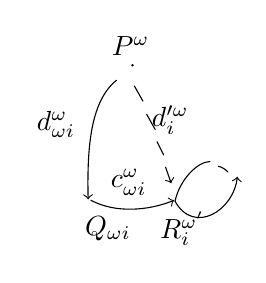
\begin{tikzpicture}[x=.012cm,y=-.012cm,line cap=round,line join=round]
\fill (128,72) circle[radius=1.4];
\draw[->] (111,88)..controls (82,111) and (80,165)..(81,214);
\draw (130,94)--(139,110);
\draw (143,124)--(152,140);
\draw (154,153)--(161,167);
\draw[->] (163,180)--(169,197);
\draw[->] (84,215)..controls (110,229) and (145,226)..(172,215);
\draw[->] (173,216)..controls (193,252) and (235,226)..(239,190);
\draw (173,216)..controls (178,193) and (197,174)..(210,174);
\draw (219,179)..controls (223,180) and (226,182)..(229,185);
\node at (126,52) {$P^\omega$};
\node at (47,135) {$d_{\omega i}^\omega$};
\node at (168,130) {$d_i^{\prime\omega}$};
\node at (124,196) {$c_{\omega i}^\omega$};
\node at (102,245) {$Q_{\omega i}$};
\node at (181,245) {$R_i^{\omega'}$};
\end{tikzpicture}}
par la formule
\margin{36}

\scanpage{38}
\mspage{(19)}
\[
(67)\qquad u(\widetilde d_i^{\prime\omega})=\varphi_i^{\omega'}(\underbrace{\xi'}_{\eta\xi})\widetilde d_i^{\prime\omega}
\]
On a aussi des chemins,
\diagram{\((66')\qquad d_i^\omega:\)\quad
\begin{tikzcd}[ampersand replacement=\&,column sep=large,row sep=large,baseline=(mainP.base)]
|[alias=mainP]| P^\omega\arrow[rr]\arrow[dr,"d_{\omega'i}^\omega"']\&\&R_i^\omega\\
\&Q_{\omega'i}\arrow[ur,"c_{\omega'i}^{\omega'}"']\&
\end{tikzcd}\qquad
\(d_i^\omega=c_{\omega'i}^{\omega'}\cdot d_{\omega'i}^\omega\)}
\margin{\diagram{\begin{tikzcd}[ampersand replacement=\&,column sep=small,row sep=large]
\&P_{\unsure{\infty}}^\omega\arrow[d,"d_{\omega'i}^\omega"]\arrow[dl,dashed]\\
R_i^\omega\&Q_{\omega'i}\arrow[l,bend left=20,"c_{\omega'i}^{\omega'}"]
\end{tikzcd}}}
\margin{NB $\tau(d_i^\omega)=d_i^{\prime\omega}$}
et on aura également
\[
(67')\qquad u(\widetilde d_i^\omega)=\varphi_i^\omega(\eta\unsure{\widetilde\sigma_\infty|\sigma_\infty}(\xi))\widetilde d_i^\omega
\]
\figure{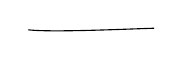
\begin{tikzpicture}\draw (0,0)..controls (.3,-.035) and (1.25,.01)..(1.6,.02);\end{tikzpicture}}

Je vois encore deux cas à regarder, savoir les sous-groupoïdes pleins de $\overline{\underline{\mathrm{VI}}}$ induits sur les \inserted{huit} sommets $(R_{i\omega},P^\omega)$, soit $\overline{\underline{\mathrm{VII}}}$, décrit par le graphe de $=$ nom et les flèches $d_i^{\prime\omega},d_i^\omega,a_i^\omega,b_i^\omega$ (24 flèches), et celui induit sur les \deleted{\unsure{cinq} points} \inserted{sommets} $Q_i,P^\omega$ --- à strictement parler, c'est le groupoïde déjà nommé $\overline{\underline{\mathrm{IV}}}$ ayant les $=$s \deleted{objets} sommets, mais
\figure{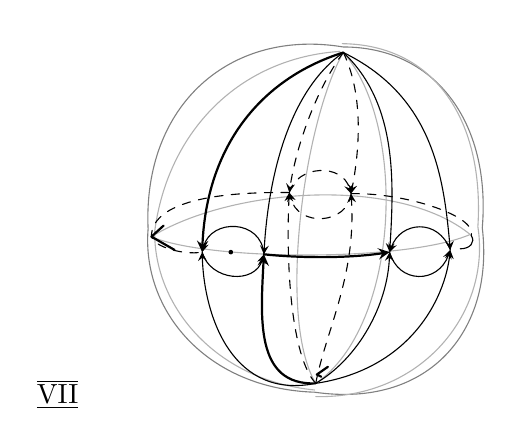
\begin{tikzpicture}[x=.014cm,y=-.014cm,line cap=round,line join=round,>=stealth]
\coordinate (N) at (192,18);\coordinate (S) at (167,318);
\coordinate (A) at (64,199);\coordinate (B) at (120,201);
\coordinate (C) at (143,145);\coordinate (D) at (199,146);
\coordinate (E) at (234,199);\coordinate (F) at (289,197);
\draw[gray,thin] (192,13)..controls (90,-4) and (10,65)..(15,178)..controls (9,253) and (69,323)..(166,326)..controls (270,341) and (329,270)..(318,177)..controls (326,81) and (275,13)..cycle;
\draw[gray!60,thin] (191,10)..controls (276,11) and (320,81)..(314,176)..controls (326,252) and (265,332)..(167,330);
\draw[gray!60,thin] (189,17)..controls (98,23) and (33,89)..(21,180)..controls (20,247) and (75,315)..(166,324);
\draw[gray!60,thin] (18,185)..controls (69,207) and (249,208)..(307,183);
\draw[gray!60,thin] (18,185)..controls (92,140) and (242,130)..(307,183);
\draw[gray!60,thin] (N)..controls (156,81) and (132,260)..(S);
\draw[gray!60,thin] (N)..controls (250,83) and (244,265)..(S);
\draw[thick,->] (N)..controls (116,42) and (68,104)..(A);
\draw[->] (N)..controls (142,53) and (124,132)..(B);
\draw[dashed,->] (N)..controls (167,52) and (149,104)..(C);
\draw[dashed,->] (N)..controls (209,53) and (208,100)..(D);
\draw[->] (N)..controls (241,64) and (238,135)..(E);
\draw[->] (N)..controls (274,58) and (283,132)..(F);
\draw[->] (S)..controls (93,333) and (66,260)..(A);
\draw[thick,->] (S)..controls (112,320) and (117,259)..(B);
\draw[dashed,->] (S)..controls (144,293) and (140,206)..(C);
\draw[thick] (178,303)--(168,310)--(172,312);
\draw[dashed,->] (S)..controls (176,271) and (204,220)..(D);
\draw[->] (S)..controls (206,295) and (232,247)..(E);
\draw[->] (S)..controls (253,305) and (284,241)..(F);
\draw[->] (B)..controls (118,169) and (72,168)..(A);
\draw[->] (A)..controls (71,225) and (112,229)..(B);
\draw[dashed,->] (C)..controls (150,120) and (191,118)..(D);
\draw[dashed,->] (D)..controls (196,174) and (151,177)..(C);
\draw[->] (F)..controls (278,168) and (244,171)..(E);
\draw[->] (E)..controls (242,228) and (278,228)..(F);
\draw[thick,->] (B)..controls (159,205) and (201,204)..(E);
\draw[dashed] (C)..controls (68,144) and (18,156)..(18,185)..controls (20,194) and (47,202)..(A);
\draw[thick] (29,175)--(18,185)--(39,197);
\draw[dashed] (D)..controls (250,145) and (314,167)..(308,184);
\draw (308,184)..controls (312,190) and (307,196)..(298,196);
\fill (90,199) circle (2.1);
\node at (-67,328) {$\overline{\underline{\mathrm{VII}}}$};
\end{tikzpicture}}
\margin{\uline{NB} les $b_i^\omega$ reliant directement les $Q_i$ sont ici inutiles}
\figure{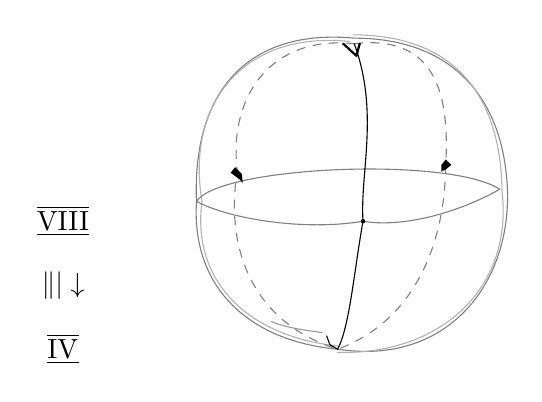
\begin{tikzpicture}[x=.014cm,y=-.014cm,line cap=round,line join=round,>=stealth]
\draw[gray,thin] (161,20)..controls (65,11) and (14,68)..(18,168)..controls (13,248) and (68,295)..(146,302)..controls (243,317) and (302,246)..(300,159)..controls (297,73) and (249,20)..cycle;
\draw[gray!60,thin] (160,17)..controls (252,17) and (294,72)..(295,159)..controls (305,243) and (244,307)..(146,305);
\draw[gray!60,thin] (157,23)..controls (61,13) and (8,79)..(23,168)..controls (13,242) and (67,291)..(146,299);
\draw[gray,thin] (18,168)..controls (39,136) and (247,127)..(293,157)..controls (254,179) and (204,192)..(169,186)..controls (116,195) and (48,184)..cycle;
\draw[gray,dashed] (161,25)..controls (82,17) and (47,77)..(55,140)..controls (43,215) and (72,279)..(146,302);
\draw[gray,dashed] (161,25)..controls (239,16) and (247,77)..(244,135)..controls (243,219) and (207,280)..(146,302);
\draw (161,25)..controls (184,87) and (166,143)..(169,186)..controls (161,230) and (157,281)..(146,302);
\draw[thick] (151,25)--(163,36)--(166,25);
\draw[gray!80] (86,277)..controls (100,283) and (119,285)..(132,287);
\draw (136,290)--(139,298)--(146,302);
\fill (53,137)--(49,142)--(57,148)--(60,151)--(59,143)--cycle;
\fill (244,130)--(240,135)--(240,141)--(244,139)--(249,135)--cycle;
\fill (169,186) circle (2.0);
\node at (-103,186) {$\overline{\underline{\mathrm{VIII}}}$};
\node at (-103,244) {$\unsure{\Vert|\downarrow}$};
\node at (-103,302) {$\overline{\underline{\mathrm{IV}}}$};
\end{tikzpicture}}
représenté par un graphe un peu plus grand --- dans $\boxed{\unsure{\mathrm{VIII}}}$ on distingue les \inserted{six} \(\underset{\rule{.5em}{.4pt}\quad\rule{.5em}{.4pt}\quad\rule{.5em}{.4pt}}{\text{\deleted{flèches}}}\) $d_i^\omega$ seulement, et on en donne \unsure{pas|par} en plus les $\widetilde a_i^\omega$, ce qui est inutile en \unsure{fait|effet} par (35). (Donc il n'est pas étonnant que dans (37), \unsure{\deleted{la}|la} donnée de $\widetilde\alpha$, qui
\margin{37}

\scanpage{39}
\mspage{(20)}
repère \inserted{les} $u(\widetilde a_i^\omega)$, résulte déjà de celle de $\xi$, qui repère \inserted{les} $u(d_i^\omega)$,
\figure{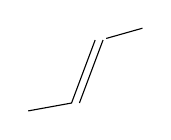
\begin{tikzpicture}[baseline=0pt]
\draw (0,0)--(.55,.10)--(.85,.90);
\draw (.65,.10)--(.95,.90);
\draw (.99,.92)--(1.45,1.05);
\end{tikzpicture}}
Les graphes $\overline{\underline{\mathrm{I}}}$ \unsure{à|:} $\overline{\underline{\mathrm{VII}}}$ donnent lieu au diagramme d'inclusions
\diagram{\begin{tikzcd}[ampersand replacement=\&,column sep=2em,row sep=2.8em,execute at end picture={
\coordinate (frameNW) at ([xshift=-4mm,yshift=5mm]\tikzcdmatrixname-2-1.north west);
\coordinate (frameSE) at ([xshift=5mm,yshift=-4mm]\tikzcdmatrixname-3-3.south east);
\coordinate (frameNE) at (frameNW -| frameSE);
\coordinate (frameSW) at (frameNW |- frameSE);
\draw ([xshift=2mm]frameNW)--([xshift=-2mm]frameNE);
\draw ([yshift=-3mm]frameNW)..controls ([yshift=-10mm]frameNW) and ([xshift=1mm,yshift=5mm]frameSW)..([xshift=1mm,yshift=2mm]frameSW);
\draw ([xshift=2mm]frameSW)--([xshift=-1mm]frameSE);
\draw ([yshift=-1mm]frameNE)--([yshift=-3mm]frameNE);
\draw ([yshift=-6mm]frameNE)--([yshift=1mm]frameSE);
\node[left=7mm] at (\tikzcdmatrixname-2-1.west) {$(68)$};
}]
\&\&\overline{\underline{\mathrm{III}}}\arrow[dl,hook']\arrow[dr,hook]\&\&\\
\overline{\underline{\mathrm{I}}}\arrow[r,hook]\arrow[dr,hook]\&\overline{\underline{\mathrm{II}}}\arrow[dr,hook]\arrow[r,phantom,"\unsure{\deleted{\leftrightarrow}|\leftrightarrow}" description]\&\phantom{\overline{\underline{\mathrm{II}}}}\&\overline{\underline{\mathrm{IV}}}\arrow[dl,hook']\&\mathrm{V}\arrow[l,hook']\\
\&\overline{\underline{\mathrm{VII}}}\arrow[r,hook]\&\overline{\underline{\mathrm{VI}}}\&\&
\end{tikzcd}}

Sans calcul, je peux déjà prédire que la donnée d'un autom. de $\overline{\underline{\mathrm{VII}}}$ fixant les sommets et commutant à $G_J$, équivaut à la donnée des quantités
\[
(69)\qquad (\uline{\lambda},\beta',\uline{\xi'})\in\widehat\Pi_{03}\times\widehat\Pi_{03}\times\widehat\Pi_{03}
\]
\margin{\(\underbrace{\begin{gathered}\text{donc }\beta'\\\text{inutile!}\end{gathered}}\)}
reliés par l\deleted{\unsure{es}}' équations \deleted{(63) ici}
\[
(70)\qquad\left\{\begin{aligned}
\beta'&=\alpha'\sigma_\infty(\lambda)\\
\beta'\sigma_\infty(\beta')&=1
\end{aligned}\right.\qquad
\begin{gathered}
\text{où}\quad\alpha'=\xi'\unsure{\rho^{\deleted{-1}}|\rho^{-1}}(\xi')^{-1}\\
\text{i.e.}\quad\alpha'\sigma_\infty(\lambda)\sigma_\infty(\alpha')\lambda=1
\end{gathered}
\]
(\unsure{tout} comme \inserted{dans le cas} $\overline{\underline{\mathrm{II}}}$ \inserted{$u$} est défini par \deleted{$(\lambda,\eta,\alpha')$},
\deleted{reliés par}
\[
(\unsure{69'})\qquad(\uline{\lambda},\uline{\eta},\alpha')\in\widehat\Pi_{0\unsure{,|.}3}\times\widehat\Pi_{03}\times\widehat\Pi_{03}
\]
avec l' équations
\margin{\begin{tabular}{@{}c@{}}donc $\alpha'$\\inutile!\end{tabular}}
\[
(70')\qquad\left\{\begin{aligned}
\beta'&=\alpha'\sigma_\infty(\lambda)\\
\alpha'\rho(\alpha')\rho^2(\alpha')&=1
\end{aligned}\right.\qquad\text{où}\quad\beta'=\eta\sigma_\infty(\eta)^{-1}
\]
\margin{38}

\scanpage{40}
\mspage{21}
Je vais expliciter les calculs $\underset{\unsure{\wedge}}{\vphantom{x}}$ dans le groupoïde $\overline{\underline{\mathrm{VII}}}$, associé au graphe de $=$ nom, on a des flèches génératrices
\[
(71)\qquad\left\{\begin{aligned}
\widetilde d_i^\omega&:P^\omega\mathpunct{.}\longrightarrow R_i^\omega\\
\widetilde d_i^{\prime\omega}&:P^\omega\longrightarrow R_i^{\omega'}\\
a_i^\omega&:R_i^\omega\mathbin{-}R_i^{\omega'}
\end{aligned}\right.
\]
liées par les relations
\[
(72)\qquad\left\{\begin{aligned}
(\widetilde d_i^{\prime\omega})^{-1}a_i^\omega\widetilde d_i^\omega&=1\\
(d_{\omega i}^{\prime\omega})^{-1}d_{\omega i}^{\omega'}(d_i^{\prime\omega'})^{-1}d_i^\omega&=1
\end{aligned}\right.
\]
\margin{six relations indépendantes exprimant les $\widetilde d_i^{\prime\omega}$ en termes des $\widetilde d_i^\omega$ et $a_i^\omega$, \inserted{ou les $\unsure{a_i^\omega}$ en termes des $\widetilde d_i^\omega,\unsure{\widetilde d_i^{\prime\omega}|d_i^{\prime\omega}}$.}}
\margin{en apparence six relations, mais il n'y en a que trois indépendantes, car l'équation pour $i,\omega$ et pour $(\omega i,\omega')$ est la $=$.}
\figure{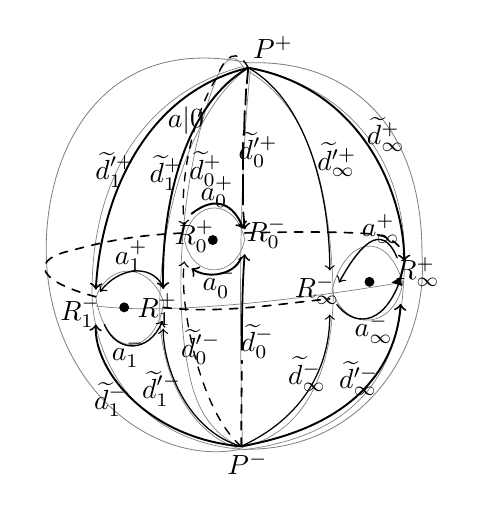
\begin{tikzpicture}[x=.009cm,y=-.009cm,line cap=round,line join=round]
\coordinate (P) at (360,1172);
\coordinate (M) at (350,1706);
\draw[gray,line width=.3pt] (360,1165)..controls (140,1120) and (65,1310)..(76,1455)..controls (90,1630) and (230,1735)..(350,1710)..controls (520,1715) and (615,1570)..(605,1435)..controls (606,1250) and (500,1160)..(360,1165);
\draw[gray,line width=.25pt] (353,1170)..controls (185,1215) and (135,1370)..(140,1503)..controls (151,1620) and (230,1700)..(348,1710);
\draw[gray,line width=.25pt] (357,1174)..controls (273,1240) and (236,1390)..(235,1510)..controls (235,1620) and (290,1695)..(350,1710);
\draw[gray,line width=.25pt] (354,1174)..controls (343,1150) and (329,1155)..(316,1185)..controls (270,1300) and (251,1480)..(276,1600)..controls (288,1664) and (317,1692)..(349,1707);
\draw[gray,line width=.25pt] (363,1176)..controls (347,1320) and (347,1530)..(352,1708);
\draw[gray,line width=.25pt] (360,1177)..controls (456,1233) and (476,1365)..(480,1492)..controls (478,1615) and (430,1690)..(352,1707);
\draw[gray,line width=.25pt] (365,1172)..controls (535,1210) and (591,1340)..(579,1475)..controls (573,1610) and (505,1692)..(352,1711);
\draw[gray,line width=.25pt] (145,1496)..controls (165,1443) and (222,1448)..(241,1503)..controls (228,1582) and (160,1585)..(145,1496);
\draw[gray,line width=.25pt] (270,1414)..controls (282,1355) and (342,1355)..(355,1414)..controls (344,1470) and (281,1473)..(270,1414);
\draw[gray,line width=.25pt] (478,1486)..controls (497,1412) and (554,1398)..(578,1475)..controls (568,1539) and (499,1548)..(478,1486);
\draw[gray,line width=.25pt] (145,1508)..controls (246,1521) and (428,1500)..(575,1475);
\draw[dashed,line width=.6pt] (145,1495)..controls (50,1470) and (60,1440)..(110,1430)..controls (180,1410) and (230,1407)..(270,1405);
\draw[dashed,line width=.6pt] (355,1405)..controls (424,1403) and (499,1403)..(540,1407)..controls (564,1412) and (576,1423)..(581,1440);
\draw[dashed,line width=.6pt] (240,1510)..controls (320,1520) and (410,1504)..(475,1498);
\fill (185,1510) circle[radius=7];
\fill (310,1415) circle[radius=7];
\fill (531,1474) circle[radius=7];
\draw[->,line width=.7pt] (P)..controls (205,1210) and (151,1370)..(145,1485);
\draw[->,line width=.7pt] (P)..controls (260,1230) and (237,1390)..(240,1484);
\draw[dashed,->,line width=.5pt] (P)..controls (345,1143) and (327,1154)..(316,1185)..controls (278,1245) and (263,1340)..(270,1395);
\draw[line width=.65pt] (P)--(358,1194);
\draw[line width=.65pt] (357,1202)--(356,1224);
\draw[line width=.65pt] (355,1233)--(354,1267);
\draw[line width=.65pt] (353,1278)--(353,1315);
\draw[line width=.65pt] (353,1323)--(353,1365);
\draw[->,line width=.65pt] (353,1376)--(355,1400);
\draw[->,line width=.45pt] (P)..controls (445,1220) and (475,1355)..(475,1458);
\draw[->,line width=.7pt] (P)..controls (520,1200) and (580,1350)..(580,1445);
\draw[->,line width=.7pt] (M)..controls (220,1695) and (142,1600)..(145,1534);
\draw[->,line width=.45pt] (M)..controls (275,1685) and (240,1595)..(240,1540);
\draw[dashed,->,line width=.5pt] (M)..controls (290,1655) and (262,1500)..(270,1445);
\draw[dashed,line width=.65pt] (M)..controls (350,1660) and (351,1615)..(351,1585);
\draw[->,line width=.65pt] (351,1570)..controls (351,1520) and (352,1470)..(355,1435);
\draw[->,line width=.45pt] (M)..controls (450,1660) and (475,1580)..(475,1520);
\draw[->,line width=.7pt] (M)..controls (525,1675) and (570,1580)..(575,1505);
\draw[->,line width=.5pt] (239,1479)..controls (221,1447) and (176,1455)..(151,1488);
\draw[->,line width=.5pt] (157,1534)..controls (174,1575) and (220,1575)..(239,1529);
\draw[->,line width=.7pt] (280,1378)..controls (315,1350) and (340,1366)..(353,1399);
\draw[->,line width=.7pt] (350,1440)..controls (340,1465) and (302,1470)..(280,1455);
\draw[->,line width=.5pt] (570,1440)..controls (548,1387) and (516,1424)..(488,1475);
\draw[line width=.5pt] (485,1506)..controls (507,1535) and (548,1540)..(573,1475);
\fill (562,1475)--(575,1467)--(577,1480)--cycle;
\node at (395,1144) {$P^+$};
\node at (359,1730) {$P^-$};
\node at (272,1246) {$\unsure{a|0}$};
\node at (123,1517) {$R_1^-$};
\node at (232,1513) {$R_1^+$};
\node at (284,1410) {$R_0^+$};
\node at (386,1405) {$R_0^-$};
\node at (457,1485) {$R_\infty^-$};
\node at (599,1460) {$R_\infty^+$};
\node at (195,1438) {$a_1^+$};
\node at (191,1573) {$a_1^-$};
\node at (316,1347) {$a_0^+$};
\node at (319,1475) {$a_0^-$};
\node at (547,1399) {$a_\infty^+$};
\node at (537,1540) {$a_\infty^-$};
\node at (172,1316) {$\widetilde d_1^{\prime+}$};
\node at (244,1320) {$\widetilde d_1^+$};
\node at (300,1315) {$\widetilde d_0^+$};
\node at (374,1288) {$\widetilde d_0^{\prime+}$};
\node at (485,1302) {$\widetilde d_\infty^{\prime+}$};
\node at (554,1266) {$\widetilde d_\infty^+$};
\node at (166,1640) {$\widetilde d_1^-$};
\node at (238,1625) {$\widetilde d_1^{\prime-}$};
\node at (293,1566) {$\widetilde d_0^{\prime-}$};
\node at (373,1558) {$\widetilde d_0^-$};
\node at (443,1604) {$\widetilde d_\infty^-$};
\node at (516,1610) {$\widetilde d_\infty^{\prime-}$};
\end{tikzpicture}}
On va repérer $u$ par les équations
\[
(\unsure{73})\qquad\left\{\begin{aligned}
u(\widetilde d_i^\omega)&=\deleted{\unsure{\widetilde d_i^\omega}}\varphi_i^\omega(\xi_1^{\deleted{\unsure{1|'}}})\widetilde d_i^\omega\\
u(\widetilde d_i^{\prime\omega})&=\deleted{\unsure{\widetilde d_i^{\prime\omega}}}\varphi_i^{\omega'}(\xi')\widetilde d_i^{\prime\omega}\\
u(a_i^\omega)&=a_i^\omega\varphi_i^\omega(\lambda)
\end{aligned}\right.\qquad \xi',\xi_1^{\deleted{\unsure{'}}},\lambda\in\widehat\Pi_{03}
\]
et il reste à exprimer que $u$ satisfait les relations (72). La première s'explicite sous la forme
\[
(74)\qquad\xi'=\varepsilon_0(\lambda\xi_1)\qquad\text{i.e.}\quad\xi_1=\lambda^{-1}\cdot\varepsilon_0^{-1}(\xi')
\]
et on trouve également
\[
(75)\qquad\unsure{\deleted{\beta}|\beta}\xi_1=\beta'\sigma_\infty(\xi')
\]
\margin{où $\beta'$ défini par la condition $(65\,\unsure{a|'}))$}
Cette relations permettant de tirer $\beta'$ en termes
\margin{39}

\scanpage{41}
\mspage{22}
de $\xi',\xi_1$ ou de l'une de ces quantités seulement
\[
(75)\qquad\begin{aligned}
\beta'&=\xi_1\sigma_\infty(\xi')^{-1}=\deleted{\varepsilon_0(\lambda\xi_1)}\xi_1(\sigma_\infty\varepsilon_0)(\lambda\xi_1)^{-1}\\
&=\lambda^{-1}\cdot\varepsilon_0^{-1}(\xi')\sigma_\infty(\xi')^{-1}.
\end{aligned}
\]
de \deleted{la \unsure{dernière}} \inserted{ces} expressions de $\beta'$ on tire
\[
(75')\qquad\begin{aligned}
\sigma_\infty(\beta')&=\sigma_\infty(\xi_1)\xi'^{-1}=\sigma_\infty(\xi_1)\varepsilon_0(\lambda\xi_1)^{-1}\\
&=\sigma_\infty(\lambda)^{-1}\underbrace{\overbrace{\rho(\xi')\xi'^{-1}}^{\alpha'^{-1}}}_{\unsure{\nearrow}\quad\deleted{\unsure{\alpha'}}}
\end{aligned}
\]
et la troisième expression de $\beta'$ \deleted{donne}

\deleted{$(\unsure{77})$ Ceci dit, l'équation \unsure{que} $(72\,b)$ \unsure{équivalent}:}
\[
\deleted{(77\qquad\beta'\sigma_\infty(\beta')=1}
\]
\deleted{soit, $\sigma_\infty(\beta')$ en posant $\beta_1=\sigma_\infty(\beta')$ \unsure{pour}}
s'écrit aussi
\[
(77)\qquad\sigma_\infty(\beta')^{-1}=\alpha'\sigma_\infty(\lambda).
\]
Ceci posé, l'équation $(72\,b)$ équivaut à
\[
(\unsure{78})\qquad\beta'\sigma_\infty(\beta')=1\qquad\text{ou encore}\quad\unsure{\sigma}_\infty(\beta')^{-1}=\beta'
\]
ce qui est invariant par la substitution $\beta'\mapsto\sigma_\infty(\beta')$ \unsure{ou|\deleted{dans}} $\beta'\mapsto\beta'^{-1}$, donc posant
\inserted{\unsure{sans|(sans} supposer \unsure{vérifiée} $(*)$)}
\[
\beta_{\unsure{1}}=\sigma_\infty(\beta')^{-1}=\alpha'\sigma_\infty(\lambda)
\]
l'équation (78) équivaut à l'équation
\[
(**)\qquad\beta_2\sigma_\infty(\beta_1)=1
\]
et implique que $\beta_1=\sigma_\infty(\beta_1)^{-1}$ donc $\beta_1=\beta'$.

En résumé, on peut tout de suite poser
\[
(\unsure{79})\qquad\beta'=\alpha'\sigma_\infty(\lambda)\qquad\text{où}\quad\alpha'=\xi'\rho(\xi')^{-1}
\]
et la relation à imposer : $(\lambda,\xi')$ est, au choix,
\margin{40}

\scanpage{42}
\mspage{23}
l'égalité du $\beta'$ défini par cette équation avec celui défini par \inserted{les formules équivalentes} $(76)$ ou $(76')$ ou (77), ou

\deleted{le fait que $\beta'$ \unsure{(ce|(vu}}
l'équation (78), écrite au choix pour $\beta'$ défini par l'une des formules $(76)$ à (77), ou par la formule (79) --- ce qui donne la formulation la plus simple.
\margin{41}

\scanpage{44}
\margin{43}
\mspage{1}
\margin{Attention, notations \unsure{de ce qui suit} p.r. à celles des calculs précédents, en $\alpha,\beta,\alpha',\beta',\xi,\eta,\xi'\ldots$}
Considérons une 2-sphère conforme \inserted{$\Sigma$} avec une partie $J$ à trois éléments,
\[
(1)\qquad J\subset\Sigma,\qquad J=(R_i)_{i\in J}
\]
de sorte que le groupe $G_J$ opère sur $\Sigma$ par automorphismes \deleted{orientés} directs, \deleted{et \unsure{aussi|que}} \deleted{$\unsure{G'_J|G_J}\times\{1,\tau\}$ le groupe des} \inserted{tandis que le groupe des automorphismes} conformes de la situation $(\Sigma,J)$ est
\[
(2)\qquad\Gamma_{\Sigma,J}=\Gamma\simeq G_J\times\{1,\tau\}
\]
\margin{\uline{NB} L'antipodisme ne fait \uline{pas} partie de $\Gamma$, car il ne stabilise pas $J$}
$\tau$ est l'unique \inserted{\deleted{anti}}autom $\ne1$ \deleted{\unsure{qui est}} qui fixe les $R_i$ \deleted{\unsure{tous}} ($\tau={}$conjugaison complexe).
\margin{donc la \unsure{catégorie des} $(\Sigma,J)$ équiv. \unsure{à} celle des couples $(J,\bar\omega)$, où $J\in(\mathrm{Ens})_3$ et $\uline{\bar\omega}\in(\mathrm{Ens})_2$ cf plus bas}
Il y a sur $\Sigma$ une unique métrique riemannienne homogène invariante pour $G_J$, \inserted{à scalaire $\lambda\in\mathbb R^{\unsure{++|*+}}$ près} \deleted{pour laquelle}, qui nous permet d'identifier canoniquement $\Sigma$ à la sphère unité dans un espace vectoriel réel euclidien $E_{\unsure{3}}$. On pose
\[
(3)\qquad\left\{\begin{aligned}
\uline{\bar\omega}&=\Omega(\Sigma)\simeq\Omega(E_{\unsure{3}})\\
\uline{\omega}&=\Omega(J)\simeq\Omega(\Sigma_{\mathbb R})\\
\uline{\varepsilon}&=\Pi_0(\Sigma\setminus\Sigma_{\mathbb R})=\Pi_0(E\setminus\unsure{V|\forall})=\Pi_0((E/V)^*)
\end{aligned}\right.
\]
\margin{ens des deux orientations de $\Sigma$, ou donc de $E$}
\margin{On pourrait écrire $E(J,\uline{\bar\omega})$ $V(J,\uline{\omega})$}
\margin{\unsure{On} a
\[
\uline{\omega}\wedge\uline{\varepsilon}\wedge\uline{\bar\omega}=1
\]
i.e.
\[
(3\text{ bis})\qquad\left\{\begin{aligned}
\uline{\omega}&\simeq\uline{\varepsilon}\wedge\uline{\omega}\\
\uline{\varepsilon}&\simeq\uline{\bar\omega}\wedge\uline{\omega}\\
\uline{\bar\omega}&\simeq\uline{\omega}\wedge\uline{\varepsilon}
\end{aligned}\right.
\]
par la conv. de Stokes entre orient. d'un hémisphère et celles de \unsure{leur|son} bord, plus précis (4) ici}
$V$ est le \inserted{$\mathbb R$-}sous-espace vectoriel de $E$ engendré par les $R_J$, qui est de dimension 2, et où
\[
(4)\qquad\Sigma_{\mathbb R}=\Sigma\cap V
\]
cercle euclidien ds le plan euclidien $V$

\scanpage{45}
On aura dans $V$
\[
(4)\qquad\sum_{j\in J}R_j=0
\]
ce qui donne un isomorphisme
\[
(5)\qquad V\simeq V_J(\mathbb R)=\operatorname{Ker}(\mathbb R^J\xrightarrow[\text{somme}]{}\mathbb R)
\]
et on a, par la ${\unsure{3}}^{\text{ième}}$ formule (3)
\[
(6)\qquad\Delta=V^\perp\simeq\mathbb R(\varepsilon)
\]
\margin{``axe polair''}
\margin{orth. de $V$ dans $E$}
\margin{(isom compatible avec la structure quadratique)}
donc
\[
(7)\qquad E\simeq V_J(\mathbb R)\oplus\mathbb R(\varepsilon)
\]
\margin{isom d'espaces euclidiens}
où dans $V_J(\mathbb R)$ on prend la seule forme quadratique \inserted{$q$} pour laquelle les $R_j$ \deleted{\unsure{sont|soient}} \inserted{satisfont} \deleted{de carré \unsure{un}}
\[
q(R_j)=1
\]
\margin{Il est clair, par cette caractérisation de $q$, que l'opération naturelle de $G_J$ sur $V(J)$ \unsure{conserve} $q$.}
(prenant une base formée de $R_i,R_j$, $R_{\unsure{n|h}}$ de coordonnées $(-1,-1)$, la forme quadratique en question est $x^2-xy+y^2$)

Dans le plan euclidien $V$, les $R_i$
\(\downarrow\)
forment les sommets d'un triangle équilatéral inscrit dans le cercle unité.
L'opération de $G_J$ sur $E$ se fait par son opération \deleted{\unsure{sur}} tautologique sur $V(J)$, et l'opération par $\operatorname{sg}(g)$ sur $\Delta$:
\margin{44}

\scanpage{46}
\mspage{2}
\[
(8)\qquad g_E=\underset{\text{tautol.}}{\underset{\rule{0.35pt}{0.32ex}\rule{2em}{0.35pt}\rule{0.35pt}{0.18ex}}{g_{V_J(\mathbb R)}}}\oplus\operatorname{sg}(g)\operatorname{id}_\Delta
\]
L'opération de $\tau$ est donnée par
\[
(9)\qquad\tau_E=\operatorname{id}_{V_J(\mathbb R)}\oplus(-\operatorname{id}_\Delta)
\]
Je pose
\[
(10)\qquad\Sigma^*=\Sigma\setminus J=\Sigma-\{R_{\deleted{\unsure{j}}\inserted{i}}\mid i\in I\}
\]
et je m'intéresse au groupoïde fondamental de $\Sigma^*$, comme exercice préliminaire de syntaxe galoisienne, avant de regarder des situations \inserted{un peu} plus complexes (le triangle équilatéral remplacé par d'autres configurations riches en symétries sur la sphère, voire sur d'autres surfaces que la sphère, ou celle-ci étant remplacée par le fibré de Hopf, en vue des applications au calcul des groupoïdes de Teichmüller...).

Il est commode d'introduire une compactification de $\Sigma^*$, pour disposer \unsure{ainsi|aussi} de ``pts-base'' ``proches'' desdits $R_i$.
\margin{45}

\scanpage{47}
\margin{La construction de l'éclaté marche dans le contexte des variétés $C^\infty$ et des variétés d'ailleurs, analytiques réelles.}
Pour ceci, considérons l'éclaté réel de $\Sigma$ en $J$, soit $\Sigma'$, dans lequel l'image inverse de $i\in J$ s'identifie à \deleted{$\unsure{P(}$ l'espace} la droite projective réelle
\[
(11)\qquad\Sigma'_{R_i}\simeq P\bigl(\underset{\tikz[baseline,x=1em,y=1em]{\draw[line width=.35pt] (0,.16) .. controls (-.03,0) and (.03,0) .. (.12,0) -- (2.65,0) .. controls (2.78,0) and (2.8,.04) .. (2.8,.16);}}{T_{\Sigma,R_i}}\bigr)
\]
\margin{espace tangent à $\Sigma$ en $R_i$, identifié à $T_{\Sigma,R_i}^*/\mathbb R^*$}
qui est un cercle plongé dans la surface compacte $\Sigma'$ (qu'on peut considérer comme obtenu en enlevant de la sphère trois rondelles autour des $R_i$, et y recollant des rubans de Möbius --- on obtient une surface non orientable dont le \deleted{genre} $\chi_!$ est égal à
\[
\begin{aligned}
&\chi_!(\Sigma)\deleted{\unsure{-3}}\inserted{-3\overbrace{\chi_!(\text{rondelle ouverte})}^{1}}+3(\underbrace{\chi_!(\text{ruban Möbius})}_{0}\\
&\deleted{\unsure{\text{à}}}=2-3=-1=1-g,
\end{aligned}
\]
donc le genre est $2$).

La découpe de cette surface suivant $\bigcup\Sigma'_{R_i}$ est une surface à bord compacte, \deleted{dont} \inserted{en fait} soit $\widetilde\Sigma$, avec
\margin{$\partial\widetilde\Sigma$ un rev. double de $\coprod_i\Sigma'_{R_i}$}
\[
(12)\qquad\partial\widetilde\Sigma\simeq\coprod_{i\in I}\underset{\tikz[baseline,x=1em,y=1em]{\draw[line width=.35pt] (0,.16) .. controls (-.03,0) and (.03,0) .. (.12,0) -- (3.05,0) .. controls (3.18,0) and (3.2,.04) .. (3.2,.16);}}{TU_{\Sigma,R_i}}
\]
\margin{cercle tangent à $\Sigma$ en $R_i$, identifiable à $T_{\Sigma,R_i}^*/\mathbb R^{*+}$ noté aussi $U_i$}
\margin{$\widetilde\Sigma$ est une sphère à bord à trois trous. Notons que $\widetilde\Sigma^\circ$ a une structure conforme, mais que celle-ci ne se prolonge pas à $\widetilde\Sigma$}
\margin{46}

\scanpage{48}
\mspage{3}
On a les équivalences de catégories
\diagram{
\begin{tikzcd}[ampersand replacement=\&]
(13)\quad \operatorname{Rev\,\text{ét}}(\widetilde\Sigma) \arrow[r,"\approx","\text{équiv}"'] \& \operatorname{Rev\,\text{et}}(\widetilde\Sigma^\circ) \arrow[r,"\sim","\text{iso}"'] \& \operatorname{Rev\,\text{et}}(\Sigma^*)
\end{tikzcd}
}
déduites de l'inclusion
\[
\widetilde\Sigma^\circ \overset{\mathrm{def}}= \widetilde\Sigma\setminus\unsure{\delta|\partial}\widetilde\Sigma = \widetilde\Sigma|\Sigma^* \hookrightarrow \widetilde\Sigma
\]
et de l'isomorphisme
\[
\widetilde\Sigma^\circ \xrightarrow{\sim} \Sigma^*,
\]
d'où une équivalence entre les groupoïdes fondamentaux au sens large (\unsure{dt|dont} les objets sont les rev. étales 1-connexes)\deleted{\unsure{des}}
\[
(14)\qquad \Pi_1(\widetilde\Sigma) \longrightarrow \Pi_1(\Sigma^*)
\]
et en composant avec
\[
\Pi_1(U_i)\longrightarrow \Pi_1(\widetilde\Sigma)
\]
déduit de l'inclusion $U_i\hookrightarrow\widetilde\Sigma$, on trouve
\[
(15)\qquad \Pi_1(\deleted{\unsure{\Sigma}}U_i)\longrightarrow\Pi_1(\Sigma^*).
\]
Nous allons représenter graphiquement l'homomorphisme 14, en ``dessinant'' $\widetilde\Sigma$ sur $\Sigma^*$, comme une région qui serait contenue dans $\Sigma^*$ en lui enlevant \inserted{l'intérieur de} trois disques \inserted{fictifs} $\Delta_i$ ``infiniment petits'' \unsure{\deleted{et}|et} (s'identifiant aux disques unités des $T_{\Sigma,R_i}$ \unsure{\deleted{g}|g}, ou encore aux cônes sur les $U_i$), et on se représentera (14) comme provenant d'une telle inclusion fictive.
\margin{Plus précisément au lieu de travailler sur $\Sigma^*$, nous travaillons sur $C$ \unsure{``sphère à trous''} un peu plus grande que $\widetilde\Sigma$\unsure{,|.}}
\margin{47}

\scanpage{49}
En fait, nous allons travailler avec des éléments de $\Pi_1(\widetilde\Sigma)$ qui proviennent, soit de p\textsuperscript{ts} de $\widetilde\Sigma$, donc de p\textsuperscript{ts} de $\Sigma^*$ ou d'un des $U_i$, soit de \uline{parties} de $\widetilde\Sigma$ qui sont 1-connexes pour la top. induite par $\widetilde\Sigma$ -- en \unsure{partant|pratique} peut-être \unsure{de|des} parties \inserted{1-conn.} de $\Sigma^*$, et en les faisant ``déborder'' sur $\widetilde\Sigma$ de façon naturelle.

Le groupe $\Gamma$ opère sur la situation \inserted{$C^\infty$} $(\Sigma,J)$, donc par transport de structure sur la situation
\[
\widetilde\Sigma\longrightarrow\Sigma\unsure{.,|,}\quad J\subset\Sigma
\]
donc sur \deleted{le} (14) (15). Un aspect essentiel du travail à faire est de garder \deleted{\unsure{cette}} constamment présente à l'esprit cette opération, et d'introduire des notations et des constructions qui soient invariantes, dans le sens requis par la situation, par les opérations en question.
\margin{48}

\scanpage{50}
\mspage{4}
\figure{
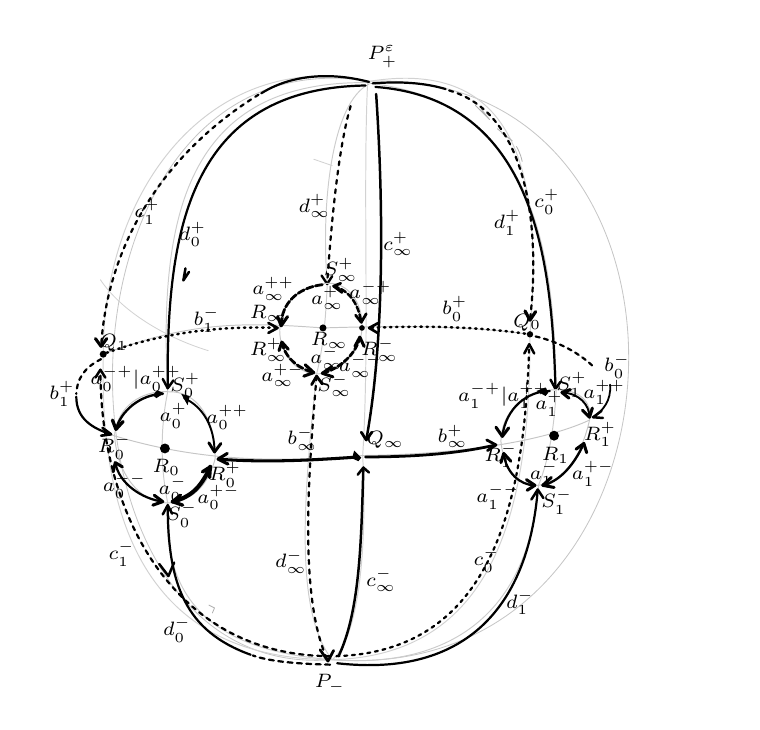
\begin{tikzpicture}[x=.009cm,y=-.009cm,>=stealth,every node/.style={font=\scriptsize},line cap=round,line join=round]
\draw[gray!45,line width=.3pt] (530,200) .. controls (63,125) and (48,1050) .. (477,1016) .. controls (1010,1055) and (1040,180) .. (530,200);
\draw[gray!35,line width=.35pt] (530,200) .. controls (310,152) and (154,347) .. (154,585) .. controls (147,879) and (256,1015) .. (477,1016);
\draw[gray!35,line width=.35pt] (530,200) .. controls (738,167) and (775,330) .. (756,557) .. controls (757,813) and (702,1010) .. (477,1016);
\draw[gray!35,line width=.35pt] (527,201) .. controls (520,349) and (530,575) .. (520,728) .. controls (527,866) and (513,988) .. (477,1016);
\draw[gray!40,line width=.35pt] (530,202) .. controls (269,197) and (232,394) .. (245,638) .. controls (234,691) and (235,747) .. (245,795) .. controls (235,951) and (333,1005) .. (477,1016);
\draw[gray!40,line width=.35pt] (530,203) .. controls (768,229) and (790,453) .. (793,635) .. controls (791,677) and (785,728) .. (768,770) .. controls (753,963) and (630,1028) .. (477,1016);
\draw[gray!40,line width=.35pt] (529,204) .. controls (476,230) and (461,374) .. (470,485) .. controls (468,537) and (464,577) .. (455,613) .. controls (436,791) and (424,949) .. (477,1016);
\draw[gray!45,line width=.35pt] (154,585) .. controls (278,538) and (355,540) .. (464,548) .. controls (591,544) and (671,546) .. (756,557);
\draw[gray!45,line width=.35pt] (166,699) .. controls (280,734) and (386,739) .. (520,728) .. controls (670,726) and (779,706) .. (840,678);
\draw[gray!35,line width=.3pt] (150,480) .. controls (178,522) and (237,560) .. (302,580);
\draw[gray!35,line width=.3pt] (451,310) -- (477,319);
\draw[gray!60,line width=.3pt] (679,234)--(699,254)--(687,239) (710,267)--(731,284)--(716,273) (737,292) .. controls (743,303) and (744,309) .. (745,313);
\draw[gray!60,line width=.3pt] (303,939)--(311,943)--(308,950);
\draw[line width=.8pt] (529,201) .. controls (476,187) and (420,190) .. (377,217);\draw[line width=.8pt,dash pattern=on 1.4pt off 1.8pt] (373,219) .. controls (239,302) and (160,430) .. (151,574);\draw[line width=1.1pt] (143,563)--(151,574)--(159,563);
\draw[line width=.8pt,dash pattern=on 1.6pt off 1.7pt] (475,1011) .. controls (260,1011) and (150,820) .. (150,607);\draw[line width=.9pt] (143,618)--(150,607)--(157,618);
\draw[line width=.8pt] (534,203) .. controls (572,200) and (607,202) .. (637,211);\draw[line width=.8pt,dash pattern=on 1.5pt off 1.7pt] (642,213) .. controls (754,245) and (771,409) .. (756,537);\draw[line width=1.15pt] (749,524)--(756,537)--(764,525);
\draw[line width=.8pt,dash pattern=on 1.1pt off 1.7pt] (483,1011) .. controls (708,1004) and (749,784) .. (755,571);\draw[line width=.9pt] (748,584)--(755,571)--(762,584);
\draw[line width=.9pt] (539,218) .. controls (550,382) and (550,572) .. (525,706);\draw[line width=1pt] (518,695)--(525,706)--(533,695);
\draw[line width=.9pt] (486,1011) .. controls (517,946) and (518,842) .. (521,745);\draw[line width=.9pt] (513,755)--(521,745)--(529,752);
\draw[line width=.8pt] (524,206) .. controls (273,210) and (243,415) .. (245,633);\draw[line width=.9pt] (270,464)--(267,481)--(275,469) (238,620)--(245,633)--(253,622);
\draw[line width=.8pt] (538,208) .. controls (763,225) and (787,453) .. (792,634);\draw[line width=.9pt] (785,621)--(792,634)--(799,624);
\draw[line width=.8pt,dash pattern=on 1.4pt off 2pt] (503,235) .. controls (486,293) and (476,396) .. (470,484);\draw[line width=.85pt] (462,474)--(470,486)--(477,475);
\draw[line width=.8pt,dash pattern=on 1.8pt off 1.6pt] (474,1023) .. controls (432,1022) and (390,1019) .. (365,1010);\draw[line width=.8pt] (362,1009) .. controls (270,976) and (245,910) .. (245,798);\draw[line width=.9pt] (238,811)--(245,798)--(251,810) (233,881)--(246,898)--(254,879);
\draw[line width=.8pt] (484,1021) .. controls (670,1042) and (754,936) .. (767,776);\draw[line width=.9pt] (758,790)--(767,776)--(775,788);
\draw[line width=.8pt,dash pattern=on 1.5pt off 2pt] (455,616) .. controls (443,758) and (430,930) .. (471,1018);\draw[line width=1pt] (448,628)--(455,616)--(463,627) (460,1002)--(471,1018)--(479,1003);
\draw[line width=.9pt,dash pattern=on .5pt off 1.7pt] (159,583) .. controls (245,552) and (329,545) .. (400,548);\draw[line width=.95pt] (387,541)--(400,548)--(387,555);
\draw[line width=.9pt,dash pattern=on .5pt off 1.7pt] (749,556) .. controls (673,545) and (593,545) .. (529,548);\draw[line width=.95pt] (542,541)--(529,548)--(541,555);
\draw[line width=1.1pt] (514,730) .. controls (445,735) and (379,738) .. (316,733);\draw[line width=1.1pt] (329,725)--(316,733)--(330,740);\fill (508,721)--(518,731)--(514,736)--(505,732)--cycle;
\draw[line width=1pt] (524,730) .. controls (594,730) and (656,725) .. (708,713);\draw[line width=1pt] (695,706)--(708,713)--(696,721);
\draw[line width=.8pt,dash pattern=on 1.5pt off 1.7pt] (151,592) .. controls (125,605) and (117,622) .. (116,641);\draw[line width=.8pt] (116,645) .. controls (116,677) and (140,690) .. (165,698);\draw[line width=.95pt] (153,689)--(165,698)--(151,700);
\draw[line width=.8pt,dash pattern=on 1.5pt off 1.6pt] (764,560) .. controls (803,569) and (831,588) .. (848,605);\draw[line width=.65pt] (869,628) .. controls (871,650) and (859,665) .. (845,674);\draw[line width=.9pt] (857,665)--(845,674)--(859,675);
\draw[gray!45,line width=.35pt] (245,638) .. controls (287,636) and (312,677) .. (312,732) .. controls (301,775) and (275,793) .. (245,795) .. controls (204,794) and (173,752) .. (170,699) .. controls (174,658) and (209,636) .. (245,638);
\draw[line width=.85pt] (238,641) .. controls (206,642) and (179,665) .. (172,691);\draw[line width=1.2pt] (167,678)--(172,691)--(182,680);\fill (230,636)--(240,640)--(229,647)--(224,643)--cycle;
\draw[line width=.7pt] (268,647) .. controls (295,659) and (311,688) .. (311,723);\draw[line width=1.05pt] (303,710)--(311,723)--(320,711);\fill (264,641)--(276,644)--(273,657)--cycle;
\draw[line width=.8pt] (171,738) .. controls (176,767) and (208,789) .. (238,793);\draw[line width=1.1pt] (168,751)--(171,738)--(181,744) (226,784)--(238,793)--(224,798);
\draw[line width=1.5pt] (305,744) .. controls (291,775) and (276,787) .. (252,793);\draw[line width=1.25pt] (294,751)--(305,744)--(304,759) (263,784)--(252,793)--(266,798);
\draw[gray!45,line width=.35pt] (793,635) .. controls (828,635) and (845,655) .. (840,678) .. controls (829,727) and (805,765) .. (768,770) .. controls (736,771) and (718,741) .. (715,708) .. controls (715,666) and (750,636) .. (793,635);
\draw[line width=.8pt] (784,637) .. controls (752,637) and (722,661) .. (717,701);\draw[line width=1.1pt] (708,688)--(717,701)--(726,689);\fill (778,632)--(765,637)--(778,644)--(782,639)--cycle;
\draw[line width=.7pt] (801,639) .. controls (826,640) and (840,657) .. (840,674);\draw[line width=1.1pt] (813,635)--(801,639)--(811,647) (830,664)--(840,674)--(844,661);
\draw[line width=.8pt] (719,725) .. controls (722,752) and (742,770) .. (763,770);\draw[line width=1.1pt] (715,738)--(719,725)--(729,736) (751,762)--(763,770)--(752,777);
\draw[line width=.85pt] (832,711) .. controls (817,744) and (796,765) .. (774,770);\draw[line width=1.1pt] (821,719)--(832,711)--(836,724) (786,759)--(774,770)--(790,773);
\draw[gray!45,line width=.35pt] (470,485) .. controls (500,483) and (521,514) .. (519,548) .. controls (518,586) and (483,612) .. (455,613) .. controls (424,611) and (403,583) .. (403,552) .. controls (402,518) and (430,487) .. (470,485);
\draw[line width=1pt,dash pattern=on 2.5pt off .9pt] (463,487) .. controls (429,491) and (405,513) .. (405,545);\draw[line width=1.1pt] (400,532)--(405,545)--(414,532);
\draw[line width=.9pt,dash pattern=on 2pt off .9pt] (479,489) .. controls (505,496) and (515,520) .. (518,540);\draw[line width=1pt] (489,485)--(479,489)--(491,498) (510,530)--(518,540)--(525,528);
\draw[line width=1pt,dash pattern=on 2.4pt off 1pt] (406,568) .. controls (411,593) and (434,607) .. (451,611);\draw[line width=1.1pt] (402,580)--(406,568)--(415,578) (439,600)--(451,611)--(437,616);
\draw[line width=1pt,dash pattern=on 2pt off .9pt] (516,561) .. controls (510,588) and (483,607) .. (463,612);\draw[line width=1.1pt] (509,574)--(516,561)--(522,574) (476,603)--(463,612)--(478,617);
\fill (154,585) circle (1.27pt);
\fill (756,557) circle (1.15pt);
\fill (241,718) circle (1.79pt);
\fill (790,700) circle (1.79pt);
\fill (464,548) circle (1.27pt);
\fill (519,548) circle (1.02pt);
\node at (548,165) {$P_+^{\deleted{\unsure{\varepsilon}}}$};
\node at (474,1050) {$P_-$};
\node at (169,569) {$Q_1$};
\node at (752,540) {$Q_0$};
\node at (552,706) {$Q_\infty$};
\node at (243,745) {$R_0$};
\node at (792,728) {$R_1$};
\node at (473,566) {$R_\infty$};
\node at (170,716) {$R_0^-$};
\node at (326,755) {$R_0^+$};
\node at (715,728) {$R_1^-$};
\node at (855,698) {$R_1^+$};
\node at (387,579) {$R_\infty^+$};
\node at (544,579) {$R_\infty^-$};
\node at (270,629) {$S_0^+$};
\node at (265,812) {$S_0^-$};
\node at (815,628) {$S_1^+$};
\node at (794,793) {$S_1^-$};
\node at (489,466) {$S_\infty^+$};
\node at (480,629) {$S_\infty^-$};
\node at (216,384) {$c_1^+$};
\node at (180,867) {$c_1^-$};
\node at (780,370) {$c_0^+$};
\node at (695,875) {$c_0^-$};
\node at (570,430) {$c_\infty^+$};
\node at (546,904) {$c_\infty^-$};
\node at (280,416) {$d_0^+$};
\node at (258,974) {$d_0^-$};
\node at (724,400) {$d_1^+$};
\node at (742,935) {$d_1^-$};
\node at (452,376) {$d_\infty^+$};
\node at (419,878) {$d_\infty^-$};
\node at (300,537) {$b_1^-$};
\node at (650,521) {$b_0^+$};
\node at (435,704) {$b_\infty^-$};
\node at (647,701) {$b_\infty^+$};
\node at (96,641) {$b_1^+$};
\node at (879,602) {$b_0^-$};
\node at (200,620) {$\unsure{a_0^{-+}|a_0^{++}}$};
\node at (329,674) {$a_0^{++}$};
\node at (184,771) {$a_0^{--}$};
\node at (317,787) {$\unsure{a_0^{+-}}$};
\node at (253,672) {$a_0^+$};
\node at (252,775) {$a_0^-$};
\node at (719,644) {$\unsure{a_1^{-+}|a_1^{++}}$};
\node at (861,639) {$a_1^{++}$};
\node at (711,786) {$\unsure{a_1^{--}}$};
\node at (845,754) {$\unsure{a_1^{+-}}$};
\node at (783,655) {$a_1^+$};
\node at (776,753) {$a_1^-$};
\node at (394,493) {$a_\infty^{++}$};
\node at (531,498) {$\unsure{a_\infty^{-+}}$};
\node at (407,615) {$\unsure{a_\infty^{+-}}$};
\node at (517,601) {$a_\infty^{--}$};
\node at (470,506) {$a_\infty^+$};
\node at (469,590) {$a_\infty^-$};
\node at (387,528) {$\deleted{\unsure{R_\infty}}$};
\end{tikzpicture}
}
On introduit
\[
(16)\quad\left\{\begin{array}{l}
Q_i\ (i\in J)^{\unsure{*}}\text{ antipodique de }R_i\ \inserted{(=-R_i)}\\
R_i^\omega\in U_i\quad(i\in J,\omega\in\uline{\omega})\\
P_\varepsilon\ \deleted{\unsure{\in}}\quad(\varepsilon\in\uline{\varepsilon}=\Pi_0(\Sigma\setminus\Sigma_{\mathbb R})\\
S_i^{\unsure{\varepsilon}}
\end{array}\right.
\]
où $P_\varepsilon$ est défini par
\[
(17)\qquad\{P_\varepsilon\}=\Delta\cap\unsure{(|\{}\Sigma-\Sigma_{\mathbb R})_\varepsilon
\]
\deleted{\unsure{des} $R_i^\omega\in U_{i\mathbb R}\unsure{\simeq\omega}$}
et $R_{i\omega}$ est défini ainsi

On a une bijection canonique
\[
(18)\qquad U_{i\mathbb R}\overset{\mathrm{def}}=\underbrace{U_i\cap T_{\Sigma_{\mathbb R},R_i}}_{TU_{\Sigma_{\mathbb R},R_i}}\simeq\omega
\]
sur \unsure{cette} variété \inserted{$\Sigma_{\mathbb R}$} de dim 1, l'une des orientations de celle-ci en les \unsure{points|point} $R_i$ (donc globalement) est en corr biunivoque avec l'une des deux directions orientées tangentes.
\margin{
\[
(19)\quad S_i^\varepsilon\in U_i\cap T_{\Sigma_i}\unsure{,}=TU_{\Sigma_i}\ \deleted{\unsure{de}}
\]
\deleted{\illegible{1} \unsure{qui}}
où $\Sigma_i$ est le grand cercle déterminé par les $P_\varepsilon^{\deleted{\unsure{\omega}}}$ et $Q_i$ on a $TU_{\Sigma_i}\simeq\uline{\varepsilon}$
Car les deux directions tangentes à $\Sigma_i$ en $R_i$ se distinguent suivant les deux hémisphères $\in\uline{\varepsilon}=\Pi_0(\Sigma\setminus\Sigma_{\mathbb R})$
}
\margin{\uline{NB} Il faudrait introduire $\widetilde\Sigma_{\deleted{\unsure{\varepsilon}}}^{(\varepsilon)}$ $(\varepsilon\in\uline{\varepsilon})$, les deux hémisphères sur $\widetilde\Sigma$, le choix des $S_i^\varepsilon$ est caractérisé par $S_i^\varepsilon\in\widetilde\Sigma_{\deleted{\unsure{\varepsilon}}}^{(\varepsilon)}$}
On a fait la figure en indexant
\[
J=\{0,1,\infty\}\qquad \uline{\omega}=\{+1,-1\}
\]
et en choisissant une orientation sur le sphère, i.e
\[
\uline{\unsure{\omega}}\simeq\{+1,-1\},\quad\text{d'où }\varepsilon\simeq\{+1,-1\}.
\]
\margin{$+$ donné par la perm. circulaire $1\to2\to3$\quad $-$ par l'inverse}
\deleted{On définit des \unsure{arcs de cercle} sur $\widetilde\Sigma$}
\deleted{\inserted{choisit des chemins}}
\deleted{\unsure{liant} des points de $\widetilde\Sigma$}
\deleted{$(19)\qquad a_i^\omega,\ b_i,\ c_i^\omega$}
\deleted{On choisit dorénavant une orientation de $\unsure{\Sigma}$}
\deleted{(pour \unsure{introduire|intérieurs} des}
\deleted{(pour les $b_i^\omega$)}
\deleted{\unsure{notations pléthoriques} \illegible{1}}
\margin{49}

\scanpage{51}
\margin{50}
\mspage{5}

\deleted{
\[
(\unsure{20|19})\qquad\uline{\bar\omega}\xrightarrow{\sim}\{\pm1\}\quad\text{\unsure{i.e.} on dispose }\uline{\omega}\xrightarrow{\sim}\uline{\varepsilon}
\]
donc dorénavant on identifie l'ens $\uline{\omega}=\Omega(J)$ \inserted{$=\Omega(\Sigma_{\mathbb R})$} avec l'ens $\uline{\varepsilon}$ des deux hémisphères.
}

\margin{Il s'agit d'\uline{arcs} de \unsure{l'un des} cercles, \unsure{qui sont déterminés} \unsure{par} origine, extrémité, désignation du parcours à priori \unsure{court|et} \unsure{ou|en} un des \unsure{sens}}

\margin{\uline{NB}
\[
\operatorname{Rep}(J)\simeq J\times\uline{\omega}
\]
\[
(i,j,k)\longmapsto(i,\omega_{i\to j\to k})\qquad(\unsure{20})
\]
le paquet $(a_i^{\omega\varepsilon})$ est un torseur sous $\Gamma=G_J\times\{1,\tau\}$
}

Introduisons sur $\widetilde\Sigma$ les \deleted{\unsure{arcs}} chemins simples : (segments orientés plongés)

\[
(\unsure{21})\qquad\overset{12}{\overset{\rule[-.2ex]{.4pt}{.6ex}\rule[.4ex]{2em}{.4pt}\rule[-.2ex]{.4pt}{.6ex}}{a_i^{\omega,\varepsilon}}},\quad\overset{6}{\overset{\rule[-.2ex]{.4pt}{.6ex}\rule[.4ex]{1.3em}{.4pt}\rule[-.2ex]{.4pt}{.6ex}}{b_i^\omega}},\quad\overset{6}{\overset{\rule[-.2ex]{.4pt}{.6ex}\rule[.4ex]{1.3em}{.4pt}\rule[-.2ex]{.4pt}{.6ex}}{c_i^\varepsilon}},\quad\overset{6}{\overset{\rule[-.2ex]{.4pt}{.6ex}\rule[.4ex]{1.3em}{.4pt}\rule[-.2ex]{.4pt}{.6ex}}{d_i^\varepsilon}},\qquad
i\in J,\ \omega\in\uline{\omega},\ \varepsilon\in\uline{\varepsilon}
\]

chaque paquet \inserted{$b,c,d$} formant un torseur sous $G_J$

\margin{\uline{NB} on a donc \deleted{\unsure{déduit}}
$g(a_i^\omega)=a_{g(i)}^{g(\omega)}$ etc}

$\tau$ opérant par
\[
(22)\quad \tau a_i^{\omega,\varepsilon}=a_i^{\omega,\unsure{\varepsilon'}},\quad
\tau b_i^\omega=b_i^\omega,\quad \tau c_i^\varepsilon=c_i^{\varepsilon'},\quad
\tau d_i^\varepsilon=d_i^{\varepsilon'}\;\raisebox{.4ex}{$\scriptstyle\unsure{\nearrow}$}.
\]

On a
\[
(23)\qquad a_i^{\omega\varepsilon}:{\unsure{S}}_i^\varepsilon\longrightarrow\deleted{\unsure{S_i^\varepsilon}}R_i^\omega\text{ sur }U_i\quad\inserted{(\text{quart de tour})}
\]
\deleted{dans le sens de l'orientation de $\Sigma$ en $R_i$}

ce qui caractérise $a_i^{\omega\varepsilon}$. \deleted{\unsure{explicite le fait q}}

\[
(24)\qquad b_i^\omega:Q_i\longrightarrow R_{\omega'i}^{\omega'}\text{ sur }\widetilde\Sigma_{\mathbb R}\simeq\deleted{\unsure{\Sigma_{\mathbb R}}}\inserted{\operatorname{\text{Déc}}(\Sigma_{\mathbb R},J)}\ \deleted{\unsure{\text{sur les}}}
\]
\deleted{(chemin d'origine \unsure{sur ce cercle}}

(chemin sur $\widetilde\Sigma_{\mathbb R}$, d'origine $Q_i$, dans la direction $\omega$, jusqu'à l'extrémité \deleted{\unsure{qui est}} du segment composante de $\widetilde\Sigma_{\mathbb R}\simeq\operatorname{\text{\unsure{Déc|Dic}}}(\Sigma_{\mathbb R},J)$, savoir $R_{\omega'i}^{\omega'}$.

\[
(25)\qquad c_i^\omega:P^\omega\mathrel{-\!\!\!-\!\!\!-}Q_i\qquad\text{suivant un arc de grand cercle}
\]

\[
(26)\qquad d_i^\omega:P^\omega\longrightarrow S_i^\omega\qquad\text{suivant un arc de grand cercle}
\]

\margin{
\[
\left.\begin{array}{l}\hline
\text{On pose aussi}\\
(27)\quad\widetilde b_i^\omega:R_{\omega i}^{\omega}\longrightarrow R_{\omega'i}^{\omega'},\quad\widetilde b_i^\omega=b_i^\omega(b_i^{\omega'})^{-1}\\\hline
\end{array}\right)
\]
\[
\left.\begin{array}{l}
\text{chemins dans}\\
\text{la direction }\omega)\\
\text{\unsure{et non pour}}\ \unsure{b_i}\\
\text{\deleted{\unsure{des points}}}\\
\text{\deleted{\illegible{2}}}\ \deleted{\unsure{b_i^\omega}}
\end{array}\right)
\]
}

Tous les arcs $\unsure{\widetilde b_i^\omega|\bar b_i^\omega},c_i^\omega,d_i^\omega$ se font sur des grands cercles de $\Sigma$, sauf que les extrémités, des $c_i^\omega,d_i^\omega$ ne sont pas dans $\Sigma^*$ mais dans \inserted{$U_i\subset$} $\partial\widetilde\Sigma\setminus\Sigma^*$

\scanpage{52}
\mspage{\unsure{6}}
Je vais introduire, dans la sphère $\widetilde\Sigma$ dont le degré de connexion est 0, cinq ouverts, pris aussi grands que possible, qui soient simplement connexes -- obtenus en pratiquant des ``coupures'' qui relient entre eux les \deleted{trois} bords $U_i$ des trois ``trous'' \deleted{$\unsure{\Sigma}$}. On pose
\figure{
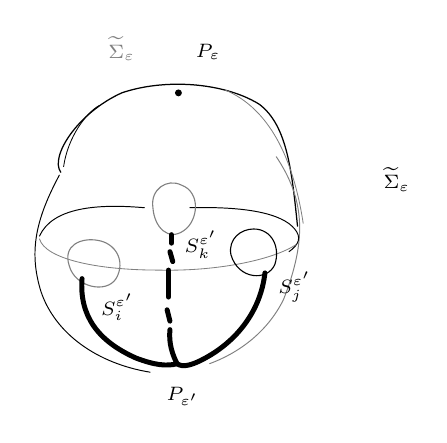
\begin{tikzpicture}[x=.018cm,y=-.018cm,every node/.style={font=\scriptsize},line cap=round,line join=round]
\draw[line width=.45pt] (33,130) .. controls (25,119) and (45,88) .. (76,74) .. controls (105,64) and (147,66) .. (173,82) .. controls (193,97) and (196,130) .. (200,168);
\draw[line width=.35pt] (32,132) .. controls (16,162) and (10,185) .. (19,214) .. controls (29,244) and (59,265) .. (96,271);
\draw[line width=.35pt,gray] (185,119) .. controls (205,149) and (207,177) .. (190,220) .. controls (178,244) and (157,258) .. (138,265);
\draw[line width=.3pt] (35,126) .. controls (38,105) and (51,88) .. (60,83);
\draw[line width=.3pt,gray] (149,72) .. controls (180,85) and (197,120) .. (204,166);
\draw[line width=.35pt] (18,175) .. controls (27,155) and (58,152) .. (92,155);
\draw[line width=.35pt] (124,155) .. controls (164,154) and (189,159) .. (198,170) .. controls (203,176) and (201,181) .. (194,186);
\draw[line width=.3pt,gray] (18,177) .. controls (22,191) and (58,199) .. (102,199) .. controls (146,200) and (184,191) .. (199,181);
\draw[line width=.4pt,gray] (39,196) .. controls (34,181) and (48,176) .. (59,178) .. controls (72,180) and (79,193) .. (72,205) .. controls (65,216) and (43,211) .. (39,196);
\draw[line width=.4pt,gray] (98,155) .. controls (96,142) and (108,134) .. (118,139) .. controls (132,144) and (130,164) .. (120,171) .. controls (109,179) and (99,169) .. (98,155);
\draw[line width=.4pt] (153,188) .. controls (151,177) and (160,170) .. (169,170) .. controls (182,170) and (188,183) .. (184,195) .. controls (179,207) and (158,206) .. (153,188);
\draw[line width=1.8pt] (48,205) .. controls (46,231) and (59,249) .. (86,261) .. controls (99,266) and (108,267) .. (115,265);
\draw[line width=1.8pt] (177,201) .. controls (174,228) and (157,249) .. (135,261) .. controls (126,266) and (119,268) .. (115,265);
\draw[line width=1.8pt] (111,174)--(111,180);
\draw[line width=1.8pt] (110,186)--(112,193);
\draw[line width=1.8pt] (109,199)--(109,218);
\draw[line width=1.8pt] (108,227)--(110,235);
\draw[line width=1.8pt] (110,241) .. controls (109,251) and (112,259) .. (115,265);
\fill (116,74) circle[radius=1.25pt];
\node[gray] at (76,43) {$\widetilde\Sigma_\varepsilon$};
\node at (137,45) {$P_\varepsilon$};
\node at (119,288) {$P_{\varepsilon'}$};
\node at (73,225) {$S_i^{\varepsilon'}$};
\node at (132,181) {$S_k^{\varepsilon'}$};
\node at (198,211) {$S_j^{\varepsilon'}$};
\node at (270,135) {$\widetilde\Sigma_\varepsilon$};
\end{tikzpicture}
}
\[
(27)\quad\left\{\begin{aligned}
\widetilde\Sigma_\varepsilon&=\widetilde\Sigma\setminus\bigcup_{i\in J}\operatorname{supp}d_i^\varepsilon \qquad\varepsilon\in\uline{\varepsilon}\\
\widetilde\Sigma_i&=\widetilde\Sigma\setminus\bigcup_{\substack{j\in J\setminus\{i\}\\\deleted{\omega\in\unsure{\uline{\omega}|\omega}}}}\deleted{\operatorname{supp}}b_i^{\unsure{\deleted{\omega}|\omega}}
\end{aligned}\right.
\]
\margin{(où $b_i=\operatorname{supp}\widetilde b_i^\omega$\newline
\deleted{$=\operatorname{supp}\unsure{c_i^\omega|b_i^\omega}\cup\operatorname{supp}\unsure{c_i^{\omega'}|b_i^{\omega'}}$}\newline
$=\operatorname{supp}c_i^\omega\cup\operatorname{supp}c_i^{\omega'}$)}
\figure{
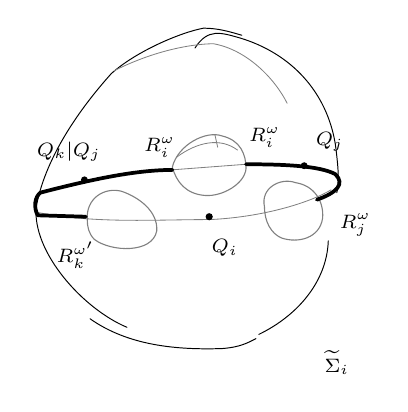
\begin{tikzpicture}[x=.018cm,y=-.018cm,every node/.style={font=\scriptsize},line cap=round,line join=round]
\draw[line width=.35pt] (73,46) .. controls (47,75) and (26,108) .. (20,140) .. controls (17,172) and (53,212) .. (84,225);
\draw[line width=.35pt] (58,219) .. controls (85,238) and (119,241) .. (151,240) .. controls (164,239) and (169,236) .. (175,233);
\draw[line width=.35pt] (132,28) .. controls (141,14) and (150,17) .. (164,21) .. controls (200,32) and (225,59) .. (231,96) .. controls (233,111) and (234,124) .. (232,130);
\draw[line width=.35pt] (226,164) .. controls (225,193) and (204,217) .. (177,230);
\draw[line width=.35pt] (73,46) .. controls (91,30) and (122,17) .. (138,14) .. controls (149,14) and (158,17) .. (165,19);
\draw[line width=.3pt,gray] (75,44) .. controls (107,28) and (134,25) .. (145,25) .. controls (168,29) and (188,49) .. (197,67);
\draw[line width=.3pt,gray] (21,144) .. controls (62,152) and (104,149) .. (143,149) .. controls (183,147) and (215,136) .. (228,128);
\draw[line width=.3pt,gray] (115,114)--(168,110);
\draw[line width=.4pt,gray] (56,149) .. controls (55,134) and (68,126) .. (80,129) .. controls (92,133) and (106,143) .. (105,157) .. controls (102,173) and (73,172) .. (61,163) .. controls (57,159) and (56,154) .. (56,149);
\draw[line width=.4pt,gray] (116,112) .. controls (120,96) and (140,86) .. (151,90) .. controls (164,93) and (168,103) .. (168,113) .. controls (167,124) and (151,133) .. (139,132) .. controls (126,131) and (119,123) .. (116,112);
\draw[line width=.3pt,gray] (119,105) .. controls (134,94) and (150,91) .. (162,100);
\draw[line width=.3pt,gray] (146,89)--(148,98);
\draw[line width=.4pt,gray] (181,140) .. controls (178,127) and (192,119) .. (203,123) .. controls (216,125) and (223,136) .. (222,148) .. controls (220,162) and (205,166) .. (193,162) .. controls (186,159) and (181,151) .. (181,140);
\draw[line width=1.35pt] (116,114) .. controls (88,114) and (54,122) .. (23,130) .. controls (19,133) and (18,140) .. (21,146)--(55,147);
\draw[line width=1.35pt] (168,110) .. controls (194,110) and (220,111) .. (231,117) .. controls (238,124) and (232,130) .. (218,135);
\fill (54,121) circle[radius=1.25pt];
\fill (142,147) circle[radius=1.3pt];
\fill (209,111) circle[radius=1.25pt];
\node at (43,101) {$\unsure{Q_k|Q_j}$};
\node at (227,94) {$Q_j$};
\node at (153,169) {$Q_i$};
\node at (107,98) {$R_i^\omega$};
\node at (181,91) {$R_i^\omega$};
\node at (48,174) {$R_k^{\omega'}$};
\node at (245,153) {$R_j^\omega$};
\node at (232,250) {$\widetilde\Sigma_i$};
\end{tikzpicture}
}
Ce sont bien des ouverts \deleted{de $\unsure{\overline{\Sigma}|\widetilde{\Sigma}}$} simplement connexes de la sphère à trous $\widetilde\Sigma$ (car le \inserted{\unsure{connexe|connexes} et à} \unsure{complémentaire|complémentaires} est connexe. On dit que $P_\omega$ est le \uline{centre} de $\widetilde\Sigma_\omega$, $Q_i$ le \uline{centre} de $\widetilde\Sigma_i$.
\margin{ce sont des ouverts denses, et pour cette raison connexes}
On pose
\[
(28)\quad\left\{\begin{aligned}
\Pi_{\unsure{\varepsilon}}&=\Pi_1(\widetilde\Sigma,\widetilde\Sigma_\varepsilon)\simeq\Pi_1(\Sigma^*,\Sigma_{\unsure{\varepsilon}}^*)\simeq\Pi_1(\Sigma^*,P_{\unsure{\varepsilon}})\\
\Pi_i&=\Pi_1(\widetilde\Sigma,\widetilde\Sigma_i)=\Pi_1(\Sigma^*,\Sigma_i^*)\simeq\Pi_1(\Sigma^*,Q_i)
\end{aligned}\right.
\]
en faisant les identifications indiquées par ces formules. \deleted{\unsure{De}} Pour $\forall\ x\in\widetilde\Sigma_\omega$ resp $x\in\widetilde\Sigma_i$, on pose
\[
(29)\quad\left\{\begin{aligned}
\varphi_{\varepsilon,x}\text{ ou }\varphi_\omega&:\Pi_\varepsilon\xrightarrow{\sim}\Pi_1(\widetilde\Sigma,x)\quad\left(\begin{gathered}\simeq\Pi_1(\Sigma^*,x)\text{ si}\\x\in\Sigma^*\end{gathered}\right)\\
\text{resp. }\varphi_{i,x}\text{ ou }\varphi_i&:\Pi_i\xrightarrow{\sim}\Pi_1(\widetilde\Sigma,x)\qquad\text{--}
\end{aligned}\right.
\]
\margin{Les $\varphi$ sont appelés \uline{isom} \uline{de} \uuline{transition}}
\margin{51}

\scanpage{53}
\mspage{6}
L'isom. canonique déduit de l'inclusion.

On a de plus des isomorphismes canoniques
\[
(30)\quad\left\{\begin{aligned}
\varphi_{i\varepsilon}&:\Pi_\omega\longrightarrow\Pi_i\qquad\text{défini par }c_i^\varepsilon:P_\varepsilon\longrightarrow Q_i\\
\varphi_{\varepsilon i}&:\Pi_i\longrightarrow\Pi_\omega\qquad\text{---}\qquad(c_i^\varepsilon)^{-1}:Q_i\longrightarrow P_\varepsilon
\end{aligned}\right.
\]
\margin{\begin{tabular}{@{}l@{}}
\uline{NB} on a\\
$\varphi_{i\varepsilon}=\varphi_{Q_i,\varepsilon}$\\
$\varphi_{\varepsilon i}=\varphi_{P_\varepsilon,i}$
\end{tabular}}
Par ces isom, les $\Pi_{\unsure{\varepsilon}},\Pi_i$ sont reliés de façon transitive, mais bien entendu pas par un syst. transitif d'isomorphismes -- au contraire, les autom d'un des groupes $\Pi_{\unsure{\varepsilon}},\Pi_i$ obtenus en composant des \unsure{isoms|isom} (30) suivant des chemins fermés sur le graphe
\figure{
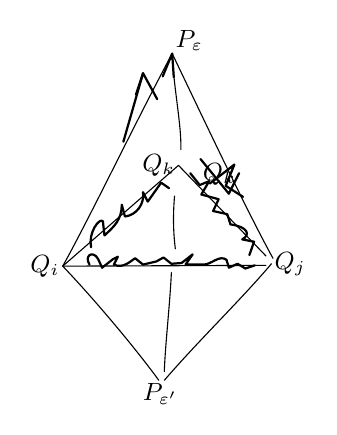
\begin{tikzpicture}[x=1cm,y=1cm,line cap=round,line join=round,every node/.style={font=\small,inner sep=1pt}]
\coordinate (P) at (.02,2.70);
\coordinate (I) at (-1.37,0);
\coordinate (J) at (1.28,.03);
\coordinate (K) at (.10,1.28);
\coordinate (M) at (-.13,-1.45);
\draw (P) .. controls (-.42,1.88) and (-1.02,.63) .. (I);
\draw (P) .. controls (.47,1.76) and (.98,.68) .. (1.30,.10);
\draw (I) .. controls (-.94,-.45) and (-.41,-1.09) .. (-.15,-1.45);
\draw (-.08,-1.45) .. controls (.35,-.95) and (.91,-.41) .. (J);
\draw (P) .. controls (.04,2.25) and (.14,1.79) .. (.13,1.48);
\draw (.05,.89) .. controls (.025,.60) and (.04,.38) .. (.06,.22);
\draw (.01,-.08) .. controls (-.01,-.50) and (-.07,-1.02) .. (-.08,-1.34);
\draw (I)--(K)--(1.21,.13);
\draw (I)--(1.21,.01);
\draw[thick] (-.60,1.58)--(-.35,2.45);
\draw[thick] (-.44,2.18)--(-.35,2.45)--(-.17,2.12);
\draw[thick] (-.10,2.41)--(.02,2.70)--(.04,2.40);
\draw[thick] (-1.01,.24).. controls (-1.05,.43) and (-.90,.62)..(-.86,.57)
  --(-.84,.39).. controls (-.72,.50) and (-.62,.59)..(-.62,.78)
  --(-.58,.63).. controls (-.43,.65) and (-.33,.79)..(-.35,.94)
  --(-.29,.82)--(-.12,1.06)--(-.02,.99);
\draw[thick] (.25,1.18)--(.37,1.03)--(.49,1.08)--(.39,.91)
  --(.61,.85)--(.54,.70)--(.72,.66)--(.76,.53)
  .. controls (.98,.50) and (1.02,.40)..(.91,.34)
  --(1.06,.31)--(1.00,.14);
\draw[thick] (-1.03,.02).. controls (-1.10,.13) and (-.99,.21)..(-.92,.09)
  --(-.87,-.02)--(-.73,.09)--(-.67,.12)--(-.72,.02)
  .. controls (-.60,-.04) and (-.49,.08)..(-.45,.10)
  --(-.35,.02)--(-.18,.06)--(-.09,.11)--(.01,.03)
  --(.14,.04)--(.28,.15)--(.19,.02)--(.42,.02)
  .. controls (.52,.02) and (.62,.15)..(.71,.08)
  --(.74,-.02)--(.85,.03)--(.95,-.03)--(1.07,.01);
\node[above right] at (P) {$P_{\unsure{\varepsilon}}$};
\node[below] at (M) {$P_{\varepsilon'}$};
\node[left] at (I) {$Q_i$};
\node[right] at (J) {$Q_j$};
\node[left] at (K) {$Q_k$};
\node at (.62,1.16) {$\deleted{\unsure{Q_k}}$};
\draw[thick] (.38,1.36)--(.74,.92)--(.87,1.18);
\draw[thick] (.50,1.05)--(.81,1.29)--(.70,1.02)--(.92,.88);
\end{tikzpicture}
}
sont \uline{tous} les autom. intérieurs !

Les $\Pi_1(\unsure{\overline{\Sigma}|\widetilde{\Sigma}}^{*},\text{en }-)$ en les $P_\varepsilon,Q_i$ étant canonifiés comme les $\Pi_\varepsilon,\Pi_i$, il reste \unsure{à|:} ``repérer'' les $\Pi_1$ en les autres sommets marqués jusqu'à maintenant. Les choix naturels sont par
\deleted{$\unsure{\varphi}_{\unsure{\omega|\varepsilon}}\ \Pi_i\quad\unsure{\varphi|\Pi}_{\unsure{\varepsilon}i}\ \Pi_i\longrightarrow$}
\margin{52}

\scanpage{54}

\[
(31)\quad\left\{\begin{aligned}
\varphi_{R_i^\omega,\omega i}&:\Pi_{\omega i}\xrightarrow{\sim}\Pi_1(\widetilde\Sigma,R_i^\omega)\\
&\text{ou }\varphi_{\omega i}\\
&\text{ou }c_{\omega i}^{\omega'}\\
\varphi_{S_i^\varepsilon,\omega\deleted{\unsure{i}}}&:\Pi_\omega\xrightarrow{\sim}\Pi_1(\widetilde\Sigma,S_i^\varepsilon)\\
&\text{ou }\varphi_\omega\\
&\text{ou }d_i^{\unsure{\varepsilon|\omega}}
\end{aligned}\right.
\]

Le plus commode me semble de noter simplement $\varphi_i,\varphi_\varepsilon$ pour préciser le groupe $\Pi_1$ standart $\Pi_i$ ou $\Pi_\varepsilon$ qui sont des sources, le point base $x$ ($=R_i^\varepsilon$ ou $S_i^\varepsilon$, disons) ne faisant pas de doute dans le calcul.

\deleted{Les arcs $a_i^\omega$ sont :}

\deleted{Les arcs $a_i^\omega$ sont visiblement trop longs, il faut les couper en deux en posant}

\[
\deleted{(31)\quad\left\{\begin{aligned}
a_i^\omega&=a_i^{\omega-}a_i^{\omega+}\\
a_i^{\omega+}&:R_{\unsure{i}}^\omega\longrightarrow S_{\unsure{i}}^\omega
\qquad a_i^{\omega-}\,\unsure{\leftarrow}:S_i^\omega\longrightarrow R_i^{\omega'}
\end{aligned}\right.}
\]

Il faut enfin, pour des calculs formels, donner une façon de repérer les $\Pi_i,\Pi_\omega$ par un $=$ groupe standart $\deleted{\unsure{\Pi_{0,3}}}$, pour lequel nous prendrons

\[
(32)\qquad\Pi_{0,3}=\Pi_{\unsure{1}}\left(\deleted{{\unsure{\Sigma}}_{\unsure{c|C}}}\overbrace{\mathbb P^1_{\mathbb C}\setminus\{0,1,\infty\}}^{U_{0,3}(\mathbb C)},P^+\right)
\]

\[
=\{l_0,l_1,l_\infty\mid l_\infty l_1l_0=1\}
\]

\[
\subset\widetilde\Pi_{03}=\Pi_1\bigl(U_{03}(\mathbb C),G_3^*\deleted{\unsure{\Pi|P}}\inserted{\times\{1,\tau\}},P^+\bigr)
\]

\[
=\{\rho,\sigma_\infty,\widetilde\sigma_\infty\mid
\rho^3=\sigma_\infty^2\inserted{=\widetilde\sigma_\infty^2\,\unsure{*}}=1,\quad
\widetilde\sigma_\infty(\rho)=\rho^{-1},\quad
\underbrace{\widetilde\sigma_\infty(\widetilde\sigma_\infty)=1}_{\inserted{\text{i.e. }(\sigma_\infty\widetilde\sigma_{\unsure{\infty}})^2=1}}\unsure{\}}
\]

\[
\deleted{=\{\rho,\unsure{\sigma_\infty}\mid\rho^3=\sigma_\infty^2=1\}\simeq\operatorname{SL}(2,\mathbb Z)/\unsure{\{\pm1\}|\pm1}}
\]

\[
\inserted{\simeq\operatorname{GL}(2,\mathbb Z)/\{\pm1\}}
\]

\margin{53}

\scanpage{55}
\mspage{7}
avec le formulaire familier dans $\widetilde\Pi_{03}\simeq\operatorname{SL}(2,\mathbb Z)$ :
\[
(33)\quad\left\{\begin{aligned}
\varepsilon_0&\overset{\text{déf}}=\sigma_\infty\unsure{\{|(}\rho\unsure{\}|\varepsilon}\\
\varepsilon_1&\overset{\text{déf}}=\rho(\varepsilon_0)\quad(=\rho\varepsilon_0\rho^{-1})\\
\varepsilon_\infty&\overset{\mathrm{def}}=\rho(\varepsilon_1)=\rho^2(\varepsilon_0)=\rho^{-1}(\varepsilon_0)
\end{aligned}\right.\qquad\begin{aligned}
l_0&\overset{\mathrm{def}}=\varepsilon_0^2\\
l_1&\overset{\text{déf}}=\varepsilon_1^2\\
l_\infty&\overset{\text{déf}}=\varepsilon_\infty^2
\end{aligned}
\]
\[
l_\infty l_1l_0=1
\]
\margin{
$\rho(l_i)=l_{\rho(i)}\quad\left\{\begin{aligned}\rho(l_0)&=l_1\\\rho(l_1)&=l_\infty\\\rho(l_\infty)&=l_0\end{aligned}\right.$\newline
$\rho(\unsure{l_i'|\varepsilon_i})=\varepsilon_{\rho(i)}$\newline
\uline{NB} on fait opérer $\rho$ sur $0,1,\infty$ par $0\mapsto1\mapsto\infty\unsure{\mapsto}0$
}
\[
(33)\quad\left\{\begin{aligned}
\dot\tau_\infty&\overset{\mathrm{def}}=\sigma_\infty\widetilde\sigma_\infty\unsure{=|,}\widetilde\sigma_\infty\sigma_\infty\\
\tau_\infty^2&=1
\end{aligned}\right.
\]
\[
\begin{aligned}\tau_\infty(l_0)&=l_0^{-1}\\\tau_\infty(l_1)&=l_1^{-1}\\
\tau_\infty(l_\infty)&\underset{\unsure{-}}{=}\unsure{l_0^{\deleted{\unsure{-1}}}|l_0^{-1}}l_1=\unsure{\operatorname{int}(l_0)}(l_\infty^{-1})
\end{aligned}
\qquad
\begin{aligned}\widetilde\sigma_\infty(l_0)&=l_1^{-1}\\\widetilde\sigma_\infty(l_1)&=l_0^{-1}\\\widetilde\sigma_\infty(l_\infty)&=l_\infty^{-1}\end{aligned}
\]
\[
\begin{aligned}\sigma_\infty(l_0)&=l_1\\\sigma_\infty(l_1)&=l_0\\\sigma_\infty(l_\infty)&=l_1^{-1}l_0^{-1}=\unsure{(}\unsure{\operatorname{int}(l_0)}(l_\infty)\end{aligned}
\]
Notons qu'un épinglage de la situation est fourni par un élément du produit
\[
\operatorname{Rep}(J,\uline{\unsure{\dot\varepsilon|\bar\omega|\varpi}})\simeq J\times\uline{\omega}\times\uline{\bar\omega}
\]
donc par la donnée d'un $(i,\omega,\bar\omega)$, définissant \deleted{donc} un $\varepsilon=\omega\wedge\bar\omega\in\uline{\varepsilon}\simeq\uline{\omega}\wedge\uline{\bar\omega}$. On va définir pour
\[
r=(\unsure{i},\omega,\underset{\deleted{\unsure{\omega|\varepsilon}}}{\bar\omega})
\]
des \unsure{isoms|isom}
\[
\deleted{\unsure{\Pi_{03}}}\qquad(34)\quad\left\{\begin{aligned}
\psi_{\deleted{\unsure{i}}\varepsilon}^{\deleted{\unsure{\omega}}i,\omega}&:\Pi_{03}\xrightarrow{\sim}\Pi_\varepsilon\\
\psi_{i\deleted{\unsure{\omega}}}^{\omega,\varepsilon}&:\Pi_{0,3}\xrightarrow{\sim}\Pi_i
\end{aligned}\right.
\]
\margin{\unsure{isoms|isom} \unsure{dits|dit} d'\uline{épinglage}}
donnant lieu comme de juste au triangle commutatif
\diagram{
\begin{tikzcd}[ampersand replacement=\&,column sep=3.2em,row sep=3.5em]
\& \Pi_{03}
\arrow[dl,"{\psi_{\deleted{\unsure{i}}\varepsilon}^{i\deleted{\unsure{\omega}}\unsure{,}\omega}}"'{pos=.46},"{\sim}"'{pos=.72}]
\arrow[dr,"{\psi_{i\deleted{\unsure{\omega}}}^{\omega,\varepsilon}}"{pos=.5},"{\sim}"{description,pos=.68,inner sep=0pt,fill=none}]
\& \\
(35)\quad\Pi_\varepsilon
\arrow[rr,shift left=1ex,"{\varphi_{i\varepsilon}}"{yshift=1ex},"{\sim}"{pos=.5,inner sep=1pt}]
\& \&
\Pi_i
\arrow[ll,shift left=1ex,"{\varphi_{\varepsilon i}}","{\sim}"'{pos=.5,inner sep=1pt},
no head,to path={
(\tikztostart) -- ([xshift=5pt]\tikztotarget.east) \tikztonodes
([xshift=4pt,yshift=2.3pt]\tikztotarget.east)
.. controls ([xshift=-.2pt,yshift=2.1pt]\tikztotarget.east)
and ([xshift=-.2pt,yshift=-2.1pt]\tikztotarget.east)
.. ([xshift=4pt,yshift=-2.3pt]\tikztotarget.east)}]
\end{tikzcd}
}
\margin{54}

\scanpage{56}
ce qui fait qu'il suffit de définir l'un des deux isom. (34) -- et en vertu de la définition de $\Pi_{03}$ dans (32), il est naturel de définir plutôt l'iso
\[
\deleted{(\unsure{35})}\qquad\psi_r=\psi_{\deleted{\unsure{\omega}}\varepsilon}^{i,\omega}:\Pi_{0,3}\xrightarrow{\sim}\Pi_\varepsilon
\]
\margin{$r=(i,\omega,\underset{\deleted{\unsure{\varepsilon}}}{\overbrace{\varepsilon,\omega}^{\bar\omega}})$}
par transport de structure comme
\[
(\unsure{36|35})\quad\left\{\begin{array}{l}
\psi_{\varepsilon\deleted{\unsure{\omega}}}^{i,\omega}=\deleted{\Pi_1(\unsure{u_{\varepsilon\omega}^{i,\omega}|u_\varepsilon^{i,\omega}})}\Pi_1(u_{i,\omega,\varepsilon};P^+)\\
\text{où }\inserted{u_r=u_{i,\omega,\varepsilon}} u_{\varepsilon\deleted{\unsure{\omega}}}^{i,\omega}:(U_{0,3}(\mathbb C)\unsure{,|;}P^{\deleted{\unsure{+}}}_{+})\longrightarrow(\Sigma^*,P_\omega).\\
\text{est l'unique iso conforme qui transforme}\\
\text{le repère \deleted{\unsure{base}} }\text{\unsure{standard|standart}}\ \inserted{\unsure{[|\{}\infty,\omega_{01\infty},+1\unsure{]|\}}}\ \text{\deleted{\unsure{analogue}} dans le}
\end{array}\right.
\]
repère $\deleted{\unsure{(\omega^2,i)|(\omega i,i)}}$ $(i,\omega,\varepsilon)$
\margin{Au couple $(i,\omega)$ on associe le repère (au sens habituel) $r=(\omega i,\omega\prime i,i)$ de $J$ i.e. \deleted{\unsure{correspondant}}\[
\begin{gathered}
0\longmapsto\omega i\\
1\longmapsto\omega^2i=\omega\prime i\\
\infty\longmapsto i
\end{gathered}
\]
Ainsi, on \unsure{a|aura}, si $r=\deleted{\unsure{(\omega i,\omega\prime i,i)}}\inserted{(i,\omega)}$\[
\rho_\omega(r)=r\circ\rho=(\omega i,\omega)
\]}

Pour un $P_\omega$ fixé, il y a six choix pour les $\inserted{\psi_r=}\ \psi_{\varepsilon\deleted{\unsure{\omega}}}^{i,\omega}:\Pi_{03}\longrightarrow\Pi_\varepsilon$ -- et pour un $Q_i$ fixé, il y a quatre choix pour $\omega,\varepsilon$. Cela fait \inserted{trois resp.} deux choix si on suppose que l'on a choisi une valeur de $\uline{\bar\omega}$ sur $\Sigma$ et réalisé donc $\uline{\varepsilon}\simeq\uline{\omega}$, et si on se borne aux $\varepsilon$ qui correspondent \unsure{à|:} $\omega\ \unsure{\Rightarrow|)}$ -- il faut donc voir comment passer de l'un \inserted{de ces choix} à l'autre.
\margin{55}

\scanpage{57}
\mspage{9}
Notons que l'isom
\[
\psi_r:\Pi_{03}\xrightarrow{\sim}\Pi_\omega
\]
\[
\inserted{\begin{gathered}
r\in\operatorname{Rep}(J,\uline{\bar\omega})\quad\text{\deleted{\unsure{pour}}}\\
\simeq\operatorname{Isom}((\Sigma_0^*,P_+),(\Sigma^*,P_+))
\end{gathered}}
\]
est compatible avec le transport des structures,
\deleted{ce qui \unsure{fait}} \inserted{donc pour} $\forall$ élément
\[
\begin{array}{rll}
g\in{}&\widetilde G_J&{}\subset\Gamma=G_J\\
&\inserted{\Vert}&\\
&\inserted{\Gamma_{P_\varepsilon}}&
\inserted{\begin{aligned}[t]
&=\left\{(g,\tau^{\unsure{\operatorname{sg}g}})\in G_J\times \deleted{\unsure{\{1,\tau\}}}\inserted{\mathbb Z/2\mathbb Z}
\ \middle|\ \begin{array}{l}
\alpha=0\text{ si }\operatorname{sg}g=1\\
\alpha=1\text{ si }\operatorname{sg}g=-1
\end{array}\right\}\\
&=\{g\in\Gamma\mid g_\varepsilon^{(\varepsilon)}=\operatorname{id}_\varepsilon\}
\end{aligned}}
\end{array}
\]
on aura commutativité de
\diagram{
\begin{tabular}{@{}c@{\qquad}c@{}}
$(37)$ &
\begin{tikzcd}[ampersand replacement=\&,column sep=large,row sep=large]
\unsure{\downarrow|\vee}\&\Pi_{03}
\arrow[dl,"{\psi_r=\psi_{\omega,i}^\varepsilon}",description]
\arrow[dr,"{\psi_{g(r)}=\psi_{g(\omega),g(i)}^{g(\varepsilon)}}"]\&\\
\Pi_{\unsure{\varepsilon}}\arrow[rr,"{\Pi_1(g)}","{\begin{gathered}\text{(par transport}\\\text{de structure}\end{gathered}}"']\&\&\Pi_\varepsilon
\end{tikzcd}
\end{tabular}
}
ce qui suffit en principe à passer d'un $\psi_r$ à
$\psi_{g(r)}=\deleted{\unsure{\varphi|\psi}}\cdot\Pi_1(g)\circ\psi_r$, vu que \deleted{\unsure{g}}
$\widetilde G_J$ est simplement transitif sur l'ens. des repères $r$
correspondant à un $\varepsilon$ fixé.
Mais on aimerait exprimer le passage par une formule de transformation
\uline{dans} $\Pi_{0,3}$.

Notons que la donnée du repère \inserted{$r$} définit un isom canonique
(encore noté ${\unsure{u}}_r$)
\margin{56}

\scanpage{58}

\[u_r:\widetilde G_3\xrightarrow{\sim}\widetilde G_3\]

et tout repère $r'$ \inserted{\unsure{avec $=$ $\varepsilon$ que $r$|au $=$ $\varepsilon$ près|avec $=$ $\varepsilon$ pour $r$}} sera de la forme de façon unique

\[r'=rg_0\quad\text{avec }g_0\in\widetilde G_3\]

\[(38)\quad\text{ie.}\quad u_{r'}=u_ru_{g_0}\qquad(\text{avec }u_r(g_0)=g\text{ mais peu importe})\]

d'où, en passant à l'action sur les $\Pi_1$ en $P_+$ resp. $P_\varepsilon$, on trouve

\[(39)\qquad\psi_{r'\deleted{\unsure{\varepsilon}}}=\psi_r\circ\Pi_1(g_0,P_+)\qquad\text{si }r'=r\circ g_0\]

\margin{$\psi_r,\psi_{r'}$ désignent ici les isom\unsure{s}\unsure{.} d'épin-\linebreak glage associés \deleted{aux} à $P_\varepsilon$}

On va expliciter ceci pour

\[g_0=\rho\quad\text{donc }r'=r\rho=(\omega i,\omega,\bar\omega)\quad\text{si }r=(i,\omega,\bar\omega)\]

On trouve

\[\psi_\varepsilon^{\omega i,\omega}=\overset{\inserted{\rho_\omega\circ\psi_\varepsilon^{i,\omega}=}}{\psi_\varepsilon^{i,\omega}\circ\rho}\]

où on a identifié $\rho$ aussi à un élément de $\widetilde\Pi_{0,3}$, et à l'autom qu'il induit sur $\Pi_{0,3}$

\uline{NB} $\rho_\omega$ est la rotation autour de $P_\varepsilon,P_{\varepsilon'}$ d'un tiers de tour, \deleted{\unsure{suivant}} l'orientation $\omega$ sur l'équateur

\margin{\uline{NB}\quad $\psi_\varepsilon^{\unsure{i|\omega},\omega}(l_0),\psi_\varepsilon^{i,\omega}(l_1),\deleted{\unsure{\psi_\varepsilon^{i,\omega}(l_0)}}$ \unsure{sont} resp. les lacets \unsure{fondés|standard|tournant} à partir de $P_\varepsilon$, autour des trous $R_{\omega i},R_{\omega^2 i}$, \deleted{\unsure{qui}} passant $Q_i$ (donc \unsure{au détriment de} $\unsure{R_{\omega i}|R_{\omega\prime i}}$ : $\unsure{R_{\omega\prime i}\cdots|R_{\omega^2 i}\cdots|R_{\omega i}\cdots}$), et dans le sens d'orientation $\bar\omega=\omega\wedge\varepsilon$}

\figure{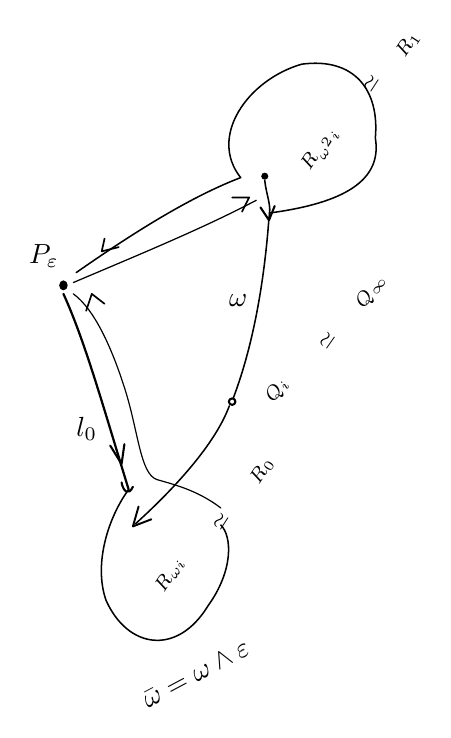
\begin{tikzpicture}[x=.018cm,y=-.018cm,line cap=round,line join=round]
\draw[line width=.55pt] (204,1700) .. controls (181,1671) and (209,1631) .. (247,1620) .. controls (284,1615) and (302,1638) .. (299,1672) .. controls (304,1702) and (277,1718) .. (224,1725);
\draw[line width=.55pt] (125,1920) .. controls (111,1939) and (100,1972) .. (109,1998) .. controls (124,2032) and (159,2038) .. (181,2002) .. controls (199,1977) and (198,1953) .. (190,1945);
\draw[line width=.55pt] (204,1700) .. controls (170,1713) and (131,1737) .. (88,1767);
\draw[line width=.60pt] (108,1743) -- (106,1752) -- (118,1749);
\draw[line width=.45pt] (86,1774) .. controls (133,1754) and (177,1736) .. (215,1716);
\draw[line width=.60pt] (198,1714) -- (210,1714) -- (205,1724);
\draw[line width=.80pt] (79,1782) .. controls (94,1815) and (106,1858) .. (125,1920);
\draw[line width=.75pt] (112,1889) -- (120,1902) -- (122,1888);
\draw[line width=.75pt] (120,1915) .. controls (121,1921) and (125,1925) .. (128,1918);
\draw[line width=.43pt] (190,1933) .. controls (173,1920) and (155,1916) .. (145,1913) .. controls (133,1909) and (132,1879) .. (122,1848) .. controls (113,1820) and (101,1793) .. (86,1782);
\draw[line width=.60pt] (95,1794) -- (99,1782) -- (108,1789);
\draw[line width=.56pt] (221,1702) .. controls (222,1712) and (226,1720) .. (224,1728) .. controls (221,1769) and (214,1815) .. (199,1855);
\draw[line width=.75pt] (218,1721) -- (224,1730) -- (228,1720);
\draw[line width=.55pt] (196,1861) .. controls (185,1891) and (151,1925) .. (130,1944);
\draw[line width=.70pt] (132,1932) -- (128,1946) -- (141,1941);
\fill (79,1776) ellipse[x radius=3.0,y radius=3.5];
\fill (221,1699) circle[radius=2.5];
\draw[line width=.75pt,fill=white] (198,1858) circle[radius=2.3];
\node[anchor=south east,inner sep=.5pt] at (77,1765) {$P_\varepsilon$};
\node[anchor=center,rotate=55,font=\scriptsize,inner sep=.2pt] at (230,1850) {$Q_i$};
\node[anchor=center,rotate=55,font=\scriptsize,inner sep=.2pt] at (265,1815) {$\simeq$};
\node[anchor=center,rotate=55,font=\scriptsize,inner sep=.2pt] at (296,1780) {$Q_\infty$};
\node[anchor=center,rotate=57,font=\scriptsize,inner sep=.2pt] at (260,1680) {$R_{\omega^2 i}$};
\node[anchor=center,rotate=57,font=\scriptsize,inner sep=.2pt] at (296,1634) {$\simeq$};
\node[anchor=center,rotate=57,font=\scriptsize,inner sep=.2pt] at (322,1606) {$R_1$};
\node[anchor=center,rotate=57,font=\scriptsize,inner sep=.2pt] at (154,1980) {$R_{\omega i}$};
\node[anchor=center,rotate=57,font=\scriptsize,inner sep=.2pt] at (190,1943) {$\simeq$};
\node[anchor=center,rotate=57,font=\scriptsize,inner sep=.2pt] at (219,1907) {$R_0$};
\node[anchor=east,inner sep=.5pt] at (104,1877) {$l_0$};
\node[anchor=east,inner sep=.5pt] at (210,1787) {$\omega$};
\node[anchor=west,rotate=28,inner sep=.5pt] at (135,2070) {$\bar\omega=\omega\wedge\varepsilon$};
\end{tikzpicture}}

On trouve de $=$, pour un autom qui renverse l'orientation de $\sigma$ i.e. pour un

\[\widetilde\sigma_\infty:\quad\begin{array}{rcl}0&\longrightarrow&1\\1&\longrightarrow&0\\{}^{\unsure{\prime}}\!\infty&\longrightarrow&\infty\end{array}\qquad\deleted{\unsure{\text{la}}}\deleted{\unsure{\text{pour}|\longmapsto}}\bar\omega\longmapsto\bar\omega'\]

\deleted{$\unsure{\widetilde\sigma_\infty}$}

\[g_0=\widetilde\sigma_\infty\qquad r'=r\sigma_\infty=(\deleted{\unsure{\omega}}i,\omega',\bar\omega').\]

d'où

\[(41)\qquad\psi_\varepsilon^{\deleted{\unsure{\omega}}i,\omega'}=\overset{\inserted{\widetilde\sigma_{\unsure{\deleted{\infty}i|i}}\circ\psi_\varepsilon^{i,\omega}=}}{\psi_\varepsilon^{i,\omega}\circ\widetilde\sigma_\infty}\]

($\widetilde\sigma_i$ est la symétrie p.r. \unsure{au|du} grand cercle méridien passant par $Q_i$)

\margin{57}

\scanpage{59}
\mspage{10}
Passons au cas de $Q_i$ -- la définition \unsure{e|é}vidente \deleted{\unsure{géométrique}} des
\[
\psi_r=\psi_i^{\omega,\varepsilon}:\quad\Pi_{0,3}-\Pi_i\deleted{(\unsure{Q_i})}
\]
est
\[
\unsure{\inserted{\psi_r=}|\psi_r=}\psi_i^{\omega,\varepsilon}=\Pi_1(\underset{u_r}{\begin{array}{@{}c@{}}u_{i,\omega,\varepsilon}\\[-1.1ex]\rule{0.4pt}{0.45ex}\rule{3.4em}{0.4pt}\rule{0.4pt}{0.45ex}\end{array}};Q_\infty)
\]
\margin{\uline{NB} on identifie la \inserted{source $\Pi_1(U_{0,3};Q_\infty)$} \deleted{\unsure{source}} à $\Pi_{03}\stackrel{\mathrm{def}}=\Pi_1(U_{0,3};P_+)$ à l'aide du chemin standard $d_\infty^+$ de $P_+$ à $Q_\infty$}
\unsure{Donc} $u_r=u_{i,\omega,\varepsilon}$ est l'unique isom de $U_{0,3}$, \inserted{dans $\Sigma^*$} qui transforme le repère \deleted{fixé}. standard $(\infty,\omega_0=+1,\bar\omega_0=+1\text{ donc }\varepsilon=\omega_0\wedge\bar\omega_0=+1)$ en $r$ i.e. qui transforme $P_+$ en $P_\varepsilon$, $Q_0$ en $Q_i$, $Q_1$ en $Q_{\omega i}$. \deleted{On}
Les épinglages \deleted{\unsure{par un repère fixé}}. \inserted{$\psi_i^{\omega,\varepsilon}$ ($i$ fixé, $\omega,\varepsilon$ variables)} de $\Pi_i$ correspondent aux $u_r$ qui transforment $Q_0$ en $Q_i$, ils sont donc déterminés par composition avec des éléments
\[
g_0\in\Gamma_0=G_3\times\{1,\tau\}
\]
qui stabilisent $Q_0$ -- ces éléments \deleted{engendrent} font un groupe $\simeq\mathbb Z/2\times\mathbb Z/2$ engendré par $\sigma_\infty,\tau$, \deleted{et} On trouve encore
\[
\psi_{r'}^{\deleted{\unsure{\omega}}}=\psi_r\circ\deleted{\unsure{\psi}}\Pi_1(g_0;Q_\infty)\quad\text{si }r'=r\circ g_0
\]
où ici $\psi_{r'},\psi_r$ désignent les iso. d'épinglag\unsure{e} relatifs \unsure{à|:} $Q_i$. Il suffit d'expliciter ces formules dans les cas de $g_0=\sigma_\infty,g_0=\tau$, ce qui revient à calculer leur effet sur $\deleted{\Pi_{0,3}=}\Pi_{\unsure{1|01}}\deleted{\unsure{\varepsilon}}(U_{0,3};\unsure{Q_\infty|R_\infty})$, quand on identifie celui-ci à $\Pi_{03}=\Pi_1(U_{0,3};P_+)$, grâce au chemin $d_\infty^+$ de $P_+$ à $Q_\infty$. On sait que l'on peut
\margin{58}

\scanpage{60}
$\operatorname{int}(\sigma_\infty),\operatorname{int}(\unsure{\sigma\tau_\infty|\tau_\infty})$,
\inserted{Or dans ce cas $g_0=\tau_\infty$\unsure{,} resp. $g_0=\sigma_\infty$, \deleted{\unsure{donc}} \inserted{on} trouve $r'=(i,\omega,\varepsilon')$ resp. $r'=(i,\omega',\varepsilon')$, donc}
\[
(39)\qquad\begin{cases}
\psi_i^{\omega,\varepsilon'}=\tau\circ\psi_i^{\omega,\varepsilon}=\psi_i^{\omega,\varepsilon}\circ\tau_\infty\\[5pt]
\psi_i^{\omega',\varepsilon'}=\underset{\substack{\text{transposition}\\\in G_J\text{ qui}\\\text{fixe }i}}{\underset{\rule{0.3pt}{0.45ex}\rule{1.6em}{0.3pt}\rule{0.3pt}{0.45ex}}{\sigma_i}}\circ\psi_i^{\omega,\varepsilon}=\psi_i^{\omega,\varepsilon}\circ\sigma_\infty
\end{cases}
\]
donc en composant
\[
(40)\qquad\psi_i^{\omega',\unsure{\varepsilon|\varepsilon\deleted{'}}}=\deleted{\unsure{\varepsilon|\tau}}\underset{\substack{\tau\sigma_i\\\text{sym\unsure{é|e}trie}\\\text{autour du}\\\text{grand cercle}\\\text{passant par}\\P_\varepsilon,P_{\varepsilon'},Q_i}}{\underset{\rule{0.3pt}{0.45ex}\rule{2.1em}{0.3pt}\rule{0.3pt}{0.45ex}}{\widetilde\sigma_i}}\circ\psi_i^{\omega,\varepsilon}=\psi_i^{\omega,\varepsilon}\circ\widetilde\sigma_\infty
\]
Dans tous ces calculs, suivant sans doute d'anciennes habitudes, j'ai privilégié les $P_\varepsilon$ et les $Q_i$ comme p\textsuperscript{ts} base -- alors que pour le travail que j'ai à faire, ce sont les points $R_i^\omega$ qui sont les plus cruciaux, \unsure{ou|où|car} les calculs faits en ces p\textsuperscript{ts} capturent directement les phénomènes de ``monodromie'' autour des ``trous'' $R_i$. Je vais réparer cette négligence, en introduisant, en
\margin{59}

\scanpage{61}
\mspage{11}
plus des $\deleted{\widetilde\Pi_\omega}\Pi_\omega$ et $\deleted{\widetilde\Pi_i},\Pi_i$, des régions
\[
\widetilde\Sigma_r=\widetilde\Sigma_{\deleted{\unsure{r}}i\deleted{\unsure{\omega}}}^{\omega,\varepsilon}
\]
associés aux repères $r=(i,\omega,\deleted{\unsure{\bar\omega|\varpi}}\unsure{\Rightarrow|\Sigma}\varepsilon)$ de $(J,\uline{\varepsilon})$ (ou ce qui revient au $=$, de $(J,\uline{\bar\omega})$), qu'on peut identifier, géométriquement, aux \inserted{douze} triangles-drapeaux, \inserted{$\unsure{D}_r=P_\varepsilon Q_iR_{\omega i}$} \unsure{correspondants|correspondant} à la subdivision barycentrique standard de la carte dans $\Sigma$ définie par l'équateur $\Sigma_{\mathbb R}$ et par les trois points $R_i$ sur celui-ci.
\figure{
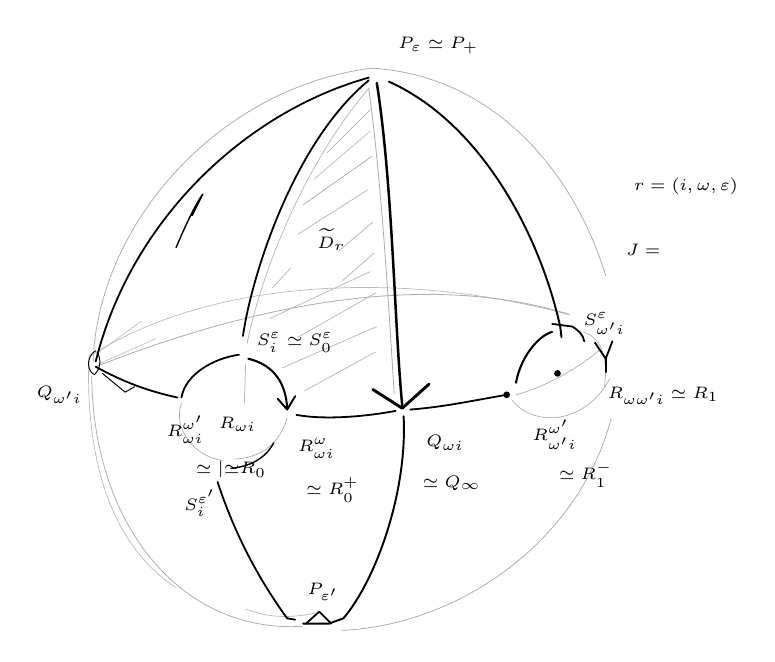
\begin{tikzpicture}[x=.017cm,y=-.017cm,line cap=round,line join=round,font=\fontsize{6}{6.5}\selectfont]
\draw[gray!65,line width=.28pt] (122,874) .. controls (126,770) and (217,669) .. (330,655) .. controls (420,660) and (481,731) .. (505,810);
\draw[gray!65,line width=.28pt] (509,917) .. controls (485,1008) and (396,1071) .. (308,1075);
\draw[gray!65,line width=.28pt] (278,1072) .. controls (188,1077) and (122,997) .. (121,885);
\draw[gray!55,line width=.25pt] (119,869) .. controls (116,935) and (130,1008) .. (184,1043);
\draw[gray!55,line width=.25pt] (236,1059) .. controls (256,1067) and (274,1065) .. (288,1062);
\draw[gray!55,line width=.25pt] (123,868) .. controls (218,809) and (363,808) .. (477,839);
\draw[gray!65,line width=.3pt] (124,878) .. controls (225,838) and (362,803) .. (478,839);
\draw[gray!50,line width=.25pt] (125,868) -- (158,844);
\draw[gray!50,line width=.25pt] (126,876) -- (169,857);
\draw[gray!55,line width=.28pt] (328,670) .. controls (284,721) and (249,801) .. (237,861);
\draw[gray!65,line width=.3pt] (328,670) .. controls (338,744) and (343,837) .. (347,898);
\draw[gray!60,line width=.28pt] (297,718) -- (329,686);
\draw[gray!50,line width=.28pt] (287,738) -- (329,702);
\draw[gray!65,line width=.28pt] (279,757) -- (330,721);
\draw[gray!55,line width=.28pt] (275,779) -- (327,746);
\draw[gray!55,line width=.28pt] (305,792) -- (331,770);
\draw[gray!55,line width=.28pt] (256,819) -- (270,804);
\draw[gray!55,line width=.28pt] (308,814) -- (332,793);
\draw[gray!55,line width=.28pt] (254,842) -- (329,807);
\draw[gray!55,line width=.28pt] (275,856) -- (333,823);
\draw[gray!55,line width=.28pt] (263,879) -- (334,848);
\draw[gray!55,line width=.28pt] (280,896) -- (333,867);
\draw[line width=.65pt] (124,874) .. controls (150,769) and (235,688) .. (328,662);
\draw[line width=.5pt] (184,789) .. controls (192,770) and (200,754) .. (204,749) -- (196,765);
\draw[line width=.7pt] (343,665) .. controls (410,695) and (455,776) .. (471,848) -- (472,856);
\draw[line width=.65pt] (328,664) .. controls (271,711) and (240,812) .. (234,855);
\draw[line width=.9pt] (334,666) .. controls (346,743) and (347,845) .. (353,907);
\draw[line width=1.05pt] (331,895) -- (353,909) -- (373,891);
\draw[line width=.7pt] (354,915) .. controls (357,972) and (333,1038) .. (309,1066) -- (298,1070) -- (279,1070);
\draw[line width=.65pt] (215,964) .. controls (230,1010) and (251,1044) .. (267,1066) -- (273,1067);
\draw[line width=.65pt] (281,1070) -- (291,1061) -- (300,1070);
\draw[line width=.65pt] (124,878) .. controls (144,889) and (162,896) .. (185,901);
\draw[line width=.35pt] (129,883) -- (146,897) -- (153,893);
\draw[line width=.35pt] (124,866) .. controls (117,870) and (117,881) .. (123,884) .. controls (128,879) and (128,872) .. (125,867);
\draw[line width=.65pt] (188,901) .. controls (191,884) and (211,872) .. (231,869);
\draw[line width=.75pt] (238,872) .. controls (258,877) and (266,891) .. (267,909);
\draw[line width=.7pt] (260,902) -- (267,910) -- (273,900);
\draw[gray!65,line width=.25pt] (188,905) .. controls (181,925) and (199,946) .. (219,948);
\draw[gray!65,line width=.25pt] (228,947) .. controls (249,946) and (262,934) .. (267,916);
\draw[line width=.5pt] (225,954) .. controls (243,952) and (252,944) .. (257,935);
\draw[gray!60,line width=.25pt] (236,876) -- (235,906);
\draw[line width=.65pt] (274,914) .. controls (296,918) and (327,915) .. (348,911);
\draw[line width=.65pt] (359,910) .. controls (385,908) and (407,903) .. (431,899);
\draw[gray!65,line width=.25pt] (435,903) .. controls (451,923) and (489,922) .. (508,887);
\draw[gray!65,line width=.25pt] (488,852) .. controls (502,856) and (507,872) .. (504,893);
\draw[gray!65,line width=.25pt] (438,899) .. controls (460,893) and (485,879) .. (501,865);
\draw[line width=.75pt] (438,890) .. controls (441,872) and (454,855) .. (465,852);
\draw[line width=.65pt] (465,846) -- (480,848) .. controls (485,851) and (488,854) .. (489,859);
\draw[line width=.65pt] (497,860) -- (505,872) -- (510,859);
\draw[line width=.65pt] (505,872) -- (505,882);
\fill (431,899) circle[radius=.425mm];
\fill (469,883) circle[radius=.425mm];
\node at (380,638) {$P_\varepsilon\simeq P_+$};
\node at (300,783) {$\widetilde{\unsure{D}}_r$};
\node[anchor=east] at (121,899) {$Q_{\omega'i}$};
\node[anchor=west] at (237,860) {$S_i^\varepsilon\simeq S_0^\varepsilon$};
\node at (191,925) {$R_{\omega i}^{\omega'}$};
\node at (289,939) {$R_{\unsure{\omega i}}^\omega$};
\node at (301,970) {$\simeq R_0^+$};
\node at (230,921) {$\unsure{R}_{\deleted{\unsure{\omega}}i}$};
\node at (225,955) {$\unsure{\simeq|\deleted{\simeq}}\deleted{\unsure{R_0}}$};
\node at (202,980) {$S_i^{\varepsilon'}$};
\node at (385,935) {$Q_{\deleted{\unsure{\omega}}i}$};
\node at (390,965) {$\simeq Q_\infty$};
\node at (504,846) {$S_{\omega'i}^\varepsilon$};
\node at (548,900) {$R_{\deleted{\unsure{\omega}}\unsure{\omega'}i}\simeq R_1$};
\node at (467,929) {$R_{\unsure{\omega'i}}^{\omega'}$};
\node at (490,959) {$\simeq R_1^-$};
\node at (294,1046) {$P_{\varepsilon'}$};
\node at (565,743) {$r=(i,\omega,\varepsilon)$};
\node at (533,791) {$J=$};
\end{tikzpicture}}
Le ``tronc'' \inserted{sur $\widetilde\Sigma$} au sens évident d'un tel triangle est un quadrilatère $\widetilde D_r$
\[
P_\varepsilon Q_{\omega'i}R_i^\omega S_i^\varepsilon\unsure{.}\simeq P_+Q_\infty R_0^+S_0^+.
\]
On aura à travail-\linebreak ler, au ``voisinage'' immédiat'' de \unsure{ces|ce} \deleted{\unsure{repères|repère}} \inserted{drapeaux} \deleted{\unsure{triangles des}} $\widetilde\Sigma_r$, avec les symétriques de $\Sigma_r$ p.r. à ses trois côtés, et se trouve sur $\widetilde\Sigma_{\unsure{\deleted{r}|r}}$, \deleted{\unsure{pour ce qui}} \inserted{ce qui conduit} à regarder la réunion de $\Sigma_r$ avec ses trois frères
\[
\tau(\Sigma_r),\widetilde\sigma_i(\Sigma_r),\widetilde\sigma_{\omega i}(\Sigma_r)
\]
(qui \inserted{resp.} correspondent, sur la sphère standard avec le repère correspondant au triangle $P_+Q_\infty R_0$, à $\tau,\widetilde\sigma_\infty,\widetilde\sigma_0$) et sur $\widetilde\Sigma$ à prendre
\[
(41)\qquad\widetilde\Sigma_r=\widetilde\Sigma_i^{\omega,\varepsilon}=\widetilde D_r\cup\tau(\widetilde D_r)\cup\widetilde\sigma_i(\widetilde D_r)\cup\widetilde\sigma_{\omega i}(\Sigma_+)
\]
limités par le contour
\[
P_\varepsilon Q_{\omega'i}R_{\omega i}^{\omega'}S_i^\varepsilon R_{\omega i}^\omega S_i^{\varepsilon'}P_{\varepsilon'}Q_iR_{\unsure{\omega'i|\omega^2i}}^{\omega'}S_{\unsure{\omega'i|\omega^2i}}^\varepsilon P_\varepsilon
\]
\margin{60}

\scanpage{62}
correspondant, sur la sphère standard, à la région ci-contre, délimitée par le contour
\[
P_+Q_1R_0^-\unsure{S_0^+|D_0^+}R_0^+S_0^-P_-Q_\infty R_1^-S_1^+P_+
\]
\figure{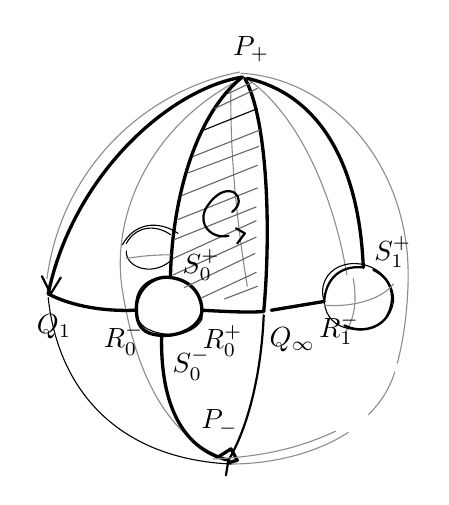
\begin{tikzpicture}[x=.016cm,y=-.016cm,line cap=round,line join=round]
\draw[thin,black!45] (219,104) .. controls (280,107) and (339,159) .. (350,239) .. controls (354,268) and (350,308) .. (343,334);
\draw[thin,black!45] (341,341) .. controls (337,354) and (330,365) .. (320,375);
\draw[thin,black!45] (304,389) .. controls (281,404) and (247,414) .. (211,414);
\draw[thin] (211,414) .. controls (123,410) and (74,357) .. (66,282);
\draw[thin,black!45] (65,267) .. controls (77,177) and (145,117) .. (218,103);
\draw[thin,black!45] (218,109) .. controls (146,146) and (115,218) .. (125,277) .. controls (136,346) and (163,395) .. (208,410);
\draw[thin,black!45] (225,109) .. controls (269,141) and (294,209) .. (303,264);
\draw[thin,black!45] (308,267) .. controls (312,288) and (307,302) .. (302,309);
\draw[thin,black!45] (211,112) .. controls (210,163) and (215,219) .. (224,273);
\draw[very thick] (220,107) .. controls (160,117) and (85,187) .. (66,279);
\draw[thick] (61,265) -- (68,279) -- (76,266);
\draw[very thick] (66,279) .. controls (85,289) and (111,293) .. (135,292);
\draw[very thick] (220,107) .. controls (180,139) and (164,211) .. (163,266);
\draw[very thick] (222,108) .. controls (240,140) and (243,228) .. (237,293);
\draw[very thick] (188,292) .. controls (207,293) and (225,294) .. (237,293);
\draw[very thick] (243,292) -- (285,285);
\draw[very thick] (224,108) .. controls (285,122) and (313,182) .. (316,258);
\draw[thin] (136,292) .. controls (133,274) and (147,264) .. (163,266) .. controls (180,269) and (190,282) .. (188,299) .. controls (182,311) and (162,315) .. (145,307) .. controls (138,303) and (135,297) .. (136,292);
\draw[very thick] (136,292) .. controls (135,277) and (148,264) .. (163,266) .. controls (179,268) and (188,279) .. (188,293);
\draw[very thick] (188,293) .. controls (186,307) and (166,315) .. (149,311) .. controls (140,309) and (136,302) .. (136,292);
\draw[thin] (128,239) .. controls (135,226) and (150,223) .. (163,232);
\draw[thin] (128,245) .. controls (127,257) and (147,266) .. (163,253);
\draw[thin] (125,240) .. controls (134,223) and (153,220) .. (169,231);
\draw[thin,black!45] (128,251) .. controls (139,249) and (151,248) .. (163,248);
\draw[thin] (285,285) .. controls (280,270) and (290,256) .. (307,255) .. controls (326,254) and (341,269) .. (340,285) .. controls (337,303) and (322,310) .. (307,307) .. controls (293,305) and (286,297) .. (285,285);
\draw[thick] (285,285) .. controls (286,268) and (297,256) .. (316,258);
\draw[thick] (324,260) .. controls (339,267) and (343,283) .. (334,298) .. controls (327,307) and (313,310) .. (301,304);
\draw[thin,black!45] (285,288) .. controls (310,290) and (332,282) .. (340,271);
\draw[very thick] (156,313) .. controls (155,364) and (171,402) .. (209,411);
\draw[thick] (237,296) .. controls (235,344) and (224,386) .. (209,411) -- (207,423);
\draw[very thick] (200,409) -- (211,402) -- (216,411) -- (209,413);
\draw[thin,black!45] (197,410) .. controls (242,408) and (270,399) .. (294,388);
\draw[thin,black!60] (209,120) -- (228,111);
\draw[thin,black!60] (198,132) -- (232,116);
\draw[thin] (187,150) -- (232,132);
\draw[thin,black!60] (181,170) -- (234,149);
\draw[thin,black!60] (177,183) -- (233,162);
\draw[thin,black!60] (172,201) -- (232,177);
\draw[thin,black!60] (169,220) -- (232,195);
\draw[thin,black!60] (166,236) -- (231,210);
\draw[thin,black!60] (165,251) -- (231,221);
\draw[thin,black!60] (165,264) -- (231,234);
\draw[thin,black!60] (174,274) -- (230,247);
\draw[thin,black!60] (188,282) -- (231,262);
\draw[thin,black!60] (206,283) -- (232,273);
\draw[thick] (212,214) .. controls (226,203) and (209,187) .. (194,207) .. controls (182,221) and (194,236) .. (209,233);
\draw[thick] (215,227) -- (222,231) -- (216,239);
\node[anchor=south] at (227,103) {$P_+$};
\node[anchor=east] at (92,305) {$Q_1$};
\node[anchor=north] at (126,295) {$R_0^-$};
\node[anchor=north west] at (181,296) {$R_0^+$};
\node[anchor=west] at (165,256) {$S_0^+$};
\node[anchor=north west] at (157,315) {$S_0^-$};
\node[anchor=north west] at (234,298) {$Q_\infty$};
\node[anchor=north] at (297,287) {$R_1^-$};
\node[anchor=west] at (317,246) {$S_1^+$};
\node[anchor=south] at (202,399) {$P_-$};
\end{tikzpicture}}
Les régions $\widetilde\Sigma_r$ sont permutées de façon simplement transitive par $\Gamma=G_J\times(1,\tau)$. Elles sont simplement connexes, et permettent donc de définir des
\[
\deleted{(42)}\qquad\Pi_r=\Pi_i^{\omega\varepsilon}=\Pi_1(\widetilde\Sigma;\widetilde\Sigma_r)=\Pi_1(\Sigma^*;\Sigma_r^*)
\]
\deleted{et des iso} \deleted{\unsure{qui}} mais qui sont reliés par un syst. transitif d'iso. à l'aide du gr. de $\Gamma$, de sorte qu'on peut identifier tous ces groupes entre eux. En fait, on trouve des isom. d'épinglage
\[
(42)\qquad\Psi_r:\Pi_{0,3}\longrightarrow\Pi_r=\Pi_i^{\omega,i}=\Pi_1(\widetilde\Sigma;\widetilde\Sigma_r)
\]
($\psi_r$ majuscule

\deleted{en \unsure{identi|ident}}
en composant
\diagram{\begin{tikzcd}[ampersand replacement=\&,column sep=large]
\Pi_{03}\arrow[r,shorten >=1.7em]\arrow[r,"\psi_r=\psi_\varepsilon^{\omega,i}"]\&
\begin{array}{c}
\Pi_1(\deleted{\unsure{P_\varepsilon|\Pi_\varepsilon}}\widetilde\Sigma,P_\varepsilon)\\
\simeq\Pi_1(\Sigma^*,P_\varepsilon)
\end{array}
\arrow[r,leftrightarrow,"\varphi_r^{-1}"]\&\Pi_r
\end{tikzcd}}
où $\deleted{\unsure{\varphi_r|\varphi}}$
\[
\varphi_r:\Pi_r\longrightarrow\Pi_\varepsilon=\Pi_1(\widetilde\Sigma,P_\varepsilon)
\]
est ``l\unsure{\deleted{a}|a}\unsure{''}'isomorphisme de transition'' correspondant à la région $1$-connexe $\Sigma_r$, et au point $P_\varepsilon$ de $\Sigma_r$.
\margin{61}

\scanpage{63}
\mspage{12}
La donnée d'un $R_{\unsure{i}}^{\unsure{\omega}}$, \inserted{qu'on va écrire $R_{\omega i}^{\omega}$, équivaut à} celle d'un repère \inserted{$r=(i,\omega)$} de $J$, et définit \uline{deux} \deleted{\unsure{rég|triang}} régions $\widetilde D_r$ qui le contiennent, correspondant aux deux repères de $(J,\uline{\varepsilon})$ qui prolongent $r$ -- et il y a donc deux régions correspondantes $\widetilde\Sigma_r$, qui sont les seules qui contiennent $R_i^\omega$ comme \uline{point intérieur} (NB. dans la région $\widetilde\Sigma_{\unsure{r_\varepsilon|r_0}}$ \unsure{standar\textsuperscript{d}|standar\textsuperscript{t}}, les deux autres points $R$ à part $R_0^+$, qui est intérieur, sont $R_0^-$ et $R_1^-$, qui ne le sont pas). Mais si la sphère $\Sigma$ est orientée i.e. si on s'est donné un élément marqué \inserted{$\bar\omega_+$} de $\uline{\bar\omega}=\uline{\omega}\wedge\uline{\varepsilon}$, ou encore un isom $\uline{\omega}\simeq\uline{\varepsilon}$, alors le point $R_i^\omega$ détermine un $\varepsilon$ \inserted{$\in\uline{\varepsilon}$} privilégié, par la condition que $\varepsilon$ corresponde à $\omega$ par $\uline{\omega}\simeq\uline{\varepsilon}$ ou encore que $\omega\wedge\varepsilon=\bar\omega_+$, ce qui signifie aussi que l'orientation $P_+S_0^+R_0^+Q_\infty P_+$ de la région $\deleted{\unsure{\widetilde\Sigma_r}}\widetilde D_r$ est \deleted{\unsure{celle de}} $\bar\omega_+$. Donc on peut alors identifier canoniquement, via $\Psi_r$, $\Pi_1(\widetilde\Sigma,R_i^\omega)$ à $\Pi_{0,3}$, par un iso (qui dépend du choix de l'orientation $\bar\omega_+$ de $\Sigma$)
\[
(43),\qquad\psi_i^\omega:\Pi_{03}\xrightarrow{\sim}\Pi_1(\widetilde\Sigma,R_i^\omega)
\]
\margin{62}

\scanpage{64}

de sorte qu'on aura \deleted{compatibilité} \inserted{commutativité} de

\diagram{\begin{tikzcd}[ampersand replacement=\&,column sep=1.6em,row sep=4.3em]
\&\Pi_{03}
 \arrow[dl,"\Psi_i^\omega"']
 \arrow[dl,no head,shift right=2pt,shorten <=18pt,shorten >=3pt,line width=.8pt,"{\deleted{\Pi_{03}}}"{description,pos=.18}]
 \arrow[d,"\psi_{\deleted{\unsure{\omega}}i}^{\omega\deleted{\unsure{\varepsilon}}}"{pos=.42}]
 \arrow[dr,"\psi_\omega^i"]\&\\
(44)\quad\Pi_0(\widetilde\Sigma,R_{\omega i}^\omega)
\&\begin{array}{c}\Pi_1(\widetilde\Sigma,Q_i)\\=\Pi_i\end{array}
 \arrow[l,"b_i^{\omega'}(\cdot)"',"{\deleted{\unsure{\rightarrow}}}"{description,pos=.08}]
\&\begin{array}{c}\Pi_1(\widetilde\Sigma,P_\omega)\\\Vert\\\Pi_\omega\end{array}
 \arrow[l,"{\begin{array}{c}\varphi_{i\omega}\\=c_i^\omega(\cdot)\end{array}}"',"{\deleted{\unsure{\rightarrow}}}"{description,pos=.08}]
 \arrow[l,no head,shift right=1pt,shorten <=2pt,shorten >=3pt,line width=.35pt]
\end{tikzcd}}

où on a écrit $P_\omega$ au lieu de $P_\varepsilon$ (en identifiant $\uline{\omega}$ et $\uline{\varepsilon}$ grâce à $\bar\omega_+$) et $\psi_i^\omega$ au lieu de $\psi_i^{\omega,\omega}$, $\psi_\omega^i$ au lieu de $\psi_\omega^{i,\omega}$.

Le passage à expliciter est celui de

\diagram{\begin{tikzcd}[ampersand replacement=\&,column sep=1.5em,row sep=2.8em]
\deleted{R_{\omega i}}\Pi_i^\omega\simeq\Pi_1(\widetilde\Sigma,R_{\omega i}^{\omega})
\&\text{à}\&\Pi_i^{\omega'}=\Pi_1(\widetilde\Sigma,R_{\omega'i}^{\omega'})\unsure{,}\\
\Pi_{0,3}\arrow[u,"\wr\;\psi_i^\omega"]\&\&\Pi_{03}\arrow[u,"\wr\;\psi_i^{\omega'}"]
\end{tikzcd}}

\inserted{Via $\widetilde b_{i\omega}$.}

\figure{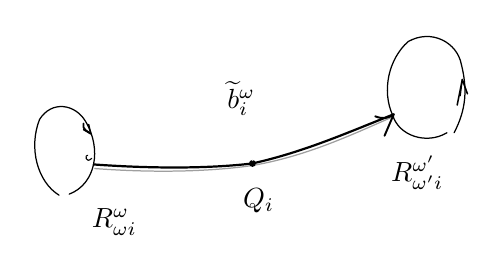
\begin{tikzpicture}[x=.013cm,y=-.013cm,line cap=round,line join=round]
\draw[line width=.45pt] (91,1384) .. controls (70,1371) and (61,1338) .. (72,1310) .. controls (84,1291) and (107,1295) .. (117,1312) .. controls (133,1339) and (127,1373) .. (101,1383);
\draw[line width=.65pt] (115,1314) .. controls (113,1320) and (120,1322) .. (122,1324);
\draw[line width=.55pt] (120,1315) -- (122,1324) -- (115,1320);
\draw[line width=.4pt] (123,1348) .. controls (117,1354) and (116,1344) .. (119,1345);
\draw[line width=.8pt] (125,1354) .. controls (195,1359) and (247,1357) .. (280,1353) .. controls (330,1342) and (375,1322) .. (418,1305);
\draw[line width=.45pt,gray!75] (126,1358) .. controls (193,1363) and (246,1360) .. (280,1355) .. controls (332,1346) and (375,1326) .. (418,1307);
\draw[line width=.7pt] (400,1307) .. controls (408,1310) and (412,1309) .. (418,1305) -- (409,1326);
\fill (280,1353) circle[radius=1.25pt];
\fill[white] (280,1350.3) circle[radius=.2pt];
\draw[line width=.45pt] (470,1323) .. controls (450,1335) and (423,1326) .. (417,1306) .. controls (406,1282) and (413,1251) .. (432,1234) .. controls (455,1221) and (480,1235) .. (484,1256) .. controls (490,1280) and (489,1300) .. (477,1323);
\draw[line width=.55pt] (480,1296) -- (485,1271) -- (490,1285);
\draw[line width=.4pt] (485,1271) -- (483,1287);
\node[above] at (269,1316) {$\widetilde b_i^\omega$};
\node[below] at (286,1368) {$Q_i$};
\node[below] at (145,1388) {$R_{\omega i}^{\omega}$};
\node[below] at (441,1336) {$R_{\omega'i}^{\unsure{\omega'}}$};
\end{tikzpicture}}

On trouve par la commutativité (44) et par la dernière formule (39) qu'on a

\deleted{$\widetilde b_{\unsure{\omega i|\omega\omega\prime}}^{\unsure{\omega}}$}

\[
(45)\qquad\widetilde b_i^\omega\bigl(\psi_i^\omega(\underset{\inserted{x}}{\deleted{\unsure{g}}})\bigr)=\psi_i^{\omega'}\bigl(\sigma_\infty(x).
\]

\margin{63}

\scanpage{66}
\margin{(\unsure{38|39} \unsure{pages|pags})}
\mspage{\unsure{5}}
Généralités sur les actions de groupes de Galois sur les compactifiés profinis de groupo\unsure{ï|i}des fondamentaux de variétés Alg. complexes
\margin{65}

\scanpage{67}
\mspage{1}
Soit $K$ un sous-corps du corps des complexes $\mathbb C$ -- des cas intéressants seront celui où $K=\mathbb Q$, ou $K$ extension finie de $\mathbb Q$, ou $K=\widetilde{\mathbb Q}$ extension abelienne maximale de $\mathbb Q$ dans $\mathbb C$ -- je serai intéressé en tous cas avant tout \unsure{aux|au} cas où $K$ est de t.f. sur $\mathbb Q$. (Le cas de $\widetilde{\mathbb Q}$ est un cas ``limite'' de tels cas, pour ne pas être gêné par les racines de $1\ldots$).

On s'intéresse aux schémas \inserted{$X$} de t.f. sur $K$, et aux espaces \inserted{analytiques} $X(\mathbb C)$ correspondants. Comme on s'intéresse aux invariants ``topologiques'' de $X,X(\mathbb C)$, on traitera les morphismes $X'-X$ qui induisent des homéom universels comme des iso -- en particulier les éléments nilpotents ne comptent pas -- une imm. fermée surjective sera traitée comme un iso.

Un langage commode est de considérer $X$ comme donné par l'espace analytique (ou $\overline{\mathrm m}$ seulement topologique) $X(\mathbb C)$, plus une \uline{structure} supplémentaire dessus : la structure de ``var. alg. sur $K$'', \unsure{a|à} coups de top. de Zariski, de faisceau des fonctions $K$-polynomiales etc. On écrira par la suite $X$ au lieu de $X(\mathbb C)$.

On distingue sur $X$ le groupoïde fondamental $\Pi_1(X)$ au sens topologique, et son compactifié profini $\widehat\Pi_1(X)$, qui \deleted{\unsure{est en un sens}} \inserted{peut} aussi être défini directement en termes du $\mathbb C$-schéma $X$. On a un foncteur ``d'inclusion''
\margin{66}

\scanpage{68}
\[
(1)\qquad\Pi_1(X)\unsure{\relbar\joinrel\relbar|\longrightarrow}\widehat\Pi_1(X)
\]
qui induit une bijection sur les ens des objets \inserted{ou ``sommets''} -- s'identifiant à $X=X(\mathbb C)$ -- et qui \deleted{\unsure{déf.|défi}} pour tt $x\in X=X(\mathbb C)$, donne l'hom de groupes
\[
(2)\qquad
\begin{array}{ccc}
\operatorname{Aut}_{\Pi_1(X)}(x)&\longrightarrow&\operatorname{Aut}_{\widehat\Pi_1(X)}(x)\\
\Vert\ \text{déf}&&\Vert\ \text{déf}\\
\pi_1(X,x)&&\widehat\pi_1(X_{\mathrm{sch}},x)
\end{array}
\]
permettant d'identifier le $\pi_1$ algébrique au compactifié profini du $\pi_1$ ``topologique'' ou ``transcendant'' : \unsure{b}
\[
(3)\qquad\pi_1(X_{\mathrm{sch}},x)\simeq\widehat\pi_1(X,x).
\]
De $=$, pour $x,y\in X$, l'application
\[
\operatorname{Hom}_{\Pi_1(X)}(x,y)\longrightarrow\operatorname{Hom}_{\widehat\Pi_1(X)\deleted{\unsure{y)|y}}}(x,y)
\]
\margin{On identifiera un élément de $\operatorname{Hom}_{\Pi_1}(x,y)$ avec son image dans $\operatorname{Hom}_{\widehat\Pi_1}(x,y)$, sans se préoccuper si l'application est injective ou non}
permet d'identifier le deuxième ens, en tant que bi-torseur sur $(\widehat\pi_1(X,y),\widehat\pi_1(X,x))$ au bitorseur déduit \deleted{Hom} du premier ens par extension des groupes d'opérateurs par
\[
\pi_1(X,y)\unsure{\relbar\joinrel\relbar|\longrightarrow}\widehat\pi_1(X,y),\qquad\pi_1(X,x)\unsure{\relbar\joinrel\relbar|\longrightarrow}\widehat\pi_1(X,x).
\]
(ce couple d'homomorphismes satisfaisant \inserted{bien} à la condition requise pour que cette extension ait un sens\ldots).
\margin{savoir (en termes de $(G,H),(G',H')$ et $G\unsure{\relbar\joinrel\relbar|\longrightarrow}G',H\to H'$ : il existe un isom ext. $G'\xrightarrow{\sim}H'$ rendant commutatif le diagramme \deleted{\unsure{des bitorseurs}}
\diagram{\begin{tikzcd}[ampersand replacement=\&,column sep=large,row sep=large]
G\arrow[r,"\sim", "\substack{\text{défini par \unsure{le}}\\\text{bitorseur }(G,H)}"']\arrow[d]\&H\arrow[d,harpoon']\\
G'\arrow[r,"\sim"]\&H'
\end{tikzcd}}}
Soit
\[
(5)\qquad\mathbf{\Gamma}_{\deleted{K}}=\mathbf{\Gamma}_K=\operatorname{Aut}_{K\text{-}\unsure{\mathrm{cor}|\mathrm{cat}}}(\mathbb C),
\]
\margin{67}

\scanpage{69}

\mspage{2}

alors $\mathbf{\Gamma}$ opère non seulement sur \deleted{$X$} l'ens. $X$, mais aussi sur le groupoïde $\widehat\Pi_1(X)$, à cause du fait que celui-ci admet une définition purement schématique, ne faisant p intervenir la topologie de $\mathbb C$. Bien entendu, si $\lambda:\deleted{\unsure{x}}x\to y$ dans $\Pi_1$, alors pour $u\in\Gamma$, $u(\lambda)$ n'est p en général une flèche de $\Pi_1$ (de $u(x)$ vers $u(y)$) mais seulement de $\widehat\Pi_1$.

\deleted{\unsure{Notation}} Notation ${}^ux$ ($x\in X,u\in\mathbf{\Gamma}$) et \deleted{\unsure{``}}

\[
\begin{array}{ll}
{}^u\lambda:{}^ux-{}^uy&\text{si }\lambda:x\to y.\\[-.4ex]
&(\text{dans }\widehat\Pi_1(X))
\end{array}
\]

On a

\diagram{\(
(6)\qquad\left\{\begin{aligned}
\unsure{{}^u(\operatorname{id}_x)|u(\operatorname{id}_x)}=\operatorname{id}_{{}^ux}&\qquad(x\in X)\\[1.2ex]
\unsure{u(\mu\lambda)|{}^u(\mu\lambda)}={}^u\mu\,{}^u\lambda&\qquad\smash{\raisebox{-1.3em}{$\left(\begin{tikzcd}[ampersand replacement=\&,column sep=2em,row sep=1.8em]
x\arrow[r,"\lambda"]\&y\arrow[r,"\mu"]\&z\\
{}^ux\arrow[r,"{}^u\lambda"]\&{}^uy\arrow[r,"{}^u\mu"]\&{}^uz
\end{tikzcd}\right)$}}
\end{aligned}\right.
\)\vspace{2.5em}}

Notre objet est d'essayer de ``déterminer'' autant que faire se peut cette action de $\mathbf{\Gamma}$. À vrai dire, si $\bar K$ est la clôture algébrique de $K$ dans $\mathbb C$, on s'intéressera surtout aux sous-groupoïdes de $\Pi_1(X)$ et $\widehat\Pi_1(X)$ induits sur l'ens d'objets $X_{\bar K}$, qu'on désignera par $\Pi_1(X_{\bar K}),\widehat\Pi_1(X_{\bar K})$ -- le deuxième est stable par l'action de $\mathbf{\Gamma}$, et si on pose

\[
(7)\qquad\Gamma=\operatorname{Aut}_{K\text{-}\unsure{\mathrm{cat}|\mathrm{cor}}}(\bar K)=\operatorname{Gal}_{\bar K/K},
\]

de sorte que $\Gamma$ est un quotient de $\mathbf{\Gamma}$, l'action de $\mathbf{\Gamma}$ sur $\Pi_1(X_{\bar K})$ se fait à travers $\Gamma$. $\uparrow$

\margin{68}

\scanpage{70}
Pour décrire l'action d'un $u\in\mathbf{\Gamma}$ (resp $u\in\Gamma$) sur $\widehat\Pi_1(X)$ (resp. \deleted{$\unsure{\Pi|\Pi_1}$} $\widehat\Pi_1(X_{\bar K})$), on prendra comme ``générateurs'' du groupoïde $\widehat\Pi_1$ des chemins provenant de $\Pi_1$. On aura, pour ${l}:x\to y$ dans $\Pi_1$, ${}^u{l}:{}^ux\unsure{\to|-}{}^uy$.

Si \deleted{\unsure{on suppose}} par la suite, pour simplifier, on se borne à des points $x,y\ldots$ rationnels sur $X$ -- i.e. qu'on travaille dans le sous-groupoïde $\widehat\Pi_1(X_K)$ $\unsure{=|?}$ formé des objets qui sont invariants sous $\mathbf{\Gamma}$ -- alors on aura
\[
(*)\qquad{}^u{l}:{}^ux=x\longrightarrow{}^uy=y,
\]
et on peut écrire, \deleted{\unsure{f}}..
\[
(8)\qquad\begin{cases}
{}^u{l}=g_{l}(u)\circ{l}={l}\circ f_{l}(u)\\
g_{l}(u)\in\widehat\pi_1(X,y)\\
f_{l}(u)\in\widehat\pi_1(X,x)
\end{cases}
\]
\deleted{$\unsure{(}\unsure{g_{l}(u)={}^u{l}\circ{l}^{-1}}$}
,\,\raisebox{0.8ex}{.}\,\raisebox{0.55ex}{.}\,\raisebox{0.4ex}{.}\,\raisebox{0.08ex}{.}
\margin{On écrira aussi parfois $g_u({l})$ au lieu de $g_{l}(u)$ $f_u({l})$ pour $f_{l}(u)$}
où $f_{l}(u),g_{l}(u),{}^u{l}$ se déterminent mutuellement, \deleted{\unsure{$f_l(u)$ et $g_l(u)$|$f_l$ et $g_l$}} par les formules (8) et
\[
(9)\qquad\begin{cases}
f_{l}(u)={l}^{-1}\cdot{}^u{l},\quad g_{l}(u)={}^u{l}\cdot{l}^{-1}\\
\unsure{g}_{l}(u)={l}(f_{l}(u)),\quad f_{l}(u)={l}^{-1}(g_{l}(u))
\end{cases}
\]
On décrira l'action d'un $u\in\Gamma$ \inserted{sur un sous-groupoïde plein de $\Pi_1(X)$} à l'aide des éléments $f_{l}(u)$, ou $g_{l}(u)$, pour un syst. de générateurs convenable des \inserted{groupoïdes pleins} \unsure{correspond.|correspondants|correspondant} de $\Pi_1(X)$. Dans le cas d'un
\margin{69}

\scanpage{71}
\mspage{3}

sous-groupoïde induit sur une partie \uline{finie} \deleted{\illegible{1}} $I$ de $X_K$, on pourra trouver un nb fini de tels générateurs --- il suffit p.ex. de choisir un \deleted{\unsure{$x$}} $x_0\in I$, et choisir pour tt $x\in I\setminus x_0$ un chemin $l_x$ de $x_0$ \unsure{à|:} $x$, et de plus un syst. \inserted{fini} de générateurs $l_i$ de $\pi_1(X,x_0)$.

\unsure{Il apparaît|Je trouvait} que sous des conditions assez générales (p.ex. si $X$ est une courbe alg. anabélienne) la connaissance de l'opération $u$ sur $\widehat{\Pi}_1(X_K,I)$ (\inserted{pour un} $u\in\Gamma$) \uline{suffit à} déterminer $u$ --- et la question se pose alors de voir comment la connaissance des invariants $g_{l_\alpha}(u)$ \inserted{disons} (pour un syst. générateur de flèches $l_\alpha$ de $\Pi_1(X,\unsure{I})$) permet de retrouver les invariants $g_l(u)$ pour d'autres \inserted{$K$-}schémas $Y\ldots$.

\margin{\figure{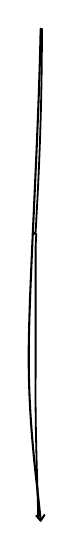
\begin{tikzpicture}[x=.08mm,y=-.08mm,line cap=round,line join=round]
\draw[line width=.65pt] (58,17) .. controls (58,180) and (50,300) .. (48,340)--(43,342)--(49,343)--(48,362) .. controls (48,430) and (48,510) .. (48,565) .. controls (47,655) and (51,738) .. (52,792);
\draw[line width=.75pt] (56,17) .. controls (52,210) and (37,430) .. (37,538) .. controls (37,650) and (50,735) .. (56,798);
\draw[line width=.75pt] (49,790)--(56,798)--(62,789);
\end{tikzpicture}}}

Quand il s'agit du $=$ schéma $X$, et qu'on s'intéresse \unsure{à|:} d'autres chemins $l:x\unsure{\relbar\joinrel\relbar|\longrightarrow}y$ $(x,y\in I)$ que les générateurs choisis $l_\alpha$, la formule (6) donne en principe un moyen de reconstituer les $g_l(u)$ pour tout $l$, puisqu'il permet de retrouver les ${}^u l$, et que ${}^u l$ est multiplicatif en $l$. En termes des $g_l(u)$, \deleted{$\unsure{=}\unsure{f_l(u)}$}, la formule de multiplicativité (6) s'écrit, pour une situation

\margin{\uline{NB} pour le moment, on ne regarde que les $x\in X_K$ qui sont dans $I$, le syst fini de points choisi\unsure{.}}

\diagram{\unsure{\begin{tikzcd}[ampersand replacement=\&,column sep=large]
x\arrow[r,no head,"l'"] \& y\arrow[r,"l^{\deleted{\unsure{''|'}}}"] \& z
\end{tikzcd}}}

\[
(10)\qquad \unsure{g_{ll'}(\deleted{ll'}u)}=g_l(u)\cdot l\bigl(g_{l'}(u)\bigr)
\qquad\text{soit }g_u(ll')=g_u(l)\cdot \unsure{l(g_u l'))|l(g_u(l'))}
\]

\margin{70}

\scanpage{72}

et en termes des $f\ldots$ la formule, est. identique mais d'allure un peu moins sympathique

\[
(11)\qquad f_{ll'}(u)=l'^{-1}\bigl(f_l(u)\bigr)\cdot f_{l'}(u)
\qquad\text{i.e. }f_u(ll')=l'^{-1}f_u(l)\cdot f_u(l')
\]

\deleted{La formule (10) peut s'exprimer en disant que pour $l$ fixé, $u\in\Gamma$ variable,}

\[
\deleted{\unsure{(17)|(12)}\qquad g_l:\Gamma\longrightarrow\widehat{\pi}_1(X,y)}
\]

\deleted{est un $1$-cocycle sur $\Gamma$, à valeurs dans $\widehat{\pi}_1(X,y)$, relativement à l'action naturelle de $\Gamma$ sur $\widehat{\pi}_1(X,y)$. Bien entendu, le $\widehat{\pi}_1(X,y)$-torseur à gauche, \inserted{\unsure{avec} op. de $\Gamma$,} correspondant à ce $1$-cocycle, n'est autre que $\operatorname{Hom}_{\widehat{\Pi}_1(X)}(x,y)$, sur lequel $\widehat{\pi}_1(X,y)=\operatorname{Hom}_{\widehat{\Pi}_1(X)}(y,y)$ opère par composition}

Pour un composé d'une \deleted{\unsure{nb} fini} suite finie composable de chemins

\diagram{\begin{tikzcd}[ampersand replacement=\&]
x_0\arrow[r,"l_1"]\&x_1\arrow[r,"l_2"]\&\cdots\&x_{n-1}\arrow[r,"l_n"]\&x_n
\end{tikzcd}}

la formule (10) prend la forme

\[
\unsure{(13)|(12)}\qquad
\begin{aligned}
g_{l_nl_{n-1}\mathinner{\ldotp\ldotp}l_1}(u)={}&g_{l_n}(u)\cdot l_n\bigl(g_{l_{n-1}}(u)\bigr)\cdot l_nl_{n-1}\bigl(g_{l_{n-2}}(u)\bigr)\mathinner{\ldotp\ldotp\ldotp\ldotp}\\
&\hfill \inserted{\cdot(l_n\mathinner{\ldotp\ldotp}l_2)g_{l_1}(u)}
\end{aligned}
\]

Formule la plus \deleted{évidente} \inserted{simple} possible en somme de celles qu'on pourrait imaginer qui \unsure{ait|ont} un sens. On va développer \deleted{\unsure{encore}} \inserted{un} contexte qui permette \deleted{\unsure{mieux|même}} d'écrire cette formule, ainsi que \deleted{(11)}, la formule analogue en $f$ et les formules

\margin{71}

\scanpage{73}
\mspage{4}
(9) de passage de $f$ à $g$, sous une forme considérablement plus simple.

Soit $T$ un espace topologique \deleted{\unsure{simplement}} $1$-connexe, et
\[
(13)\qquad p:T\longrightarrow X
\]
une application continue \inserted{(le cas injectif sera le plus intéressant)}. Soit $T_K=p^{-1}(X_K)$.

Considérons \deleted{$\unsure{\Pi_1(T)|\Pi_1(T_K)},\ \Pi_1$}
\deleted{\unsure{Soient} $x,y\in T_K$}
\[
\unsure{(14)}\qquad \deleted{\unsure{\Pi_1(X;T|\Pi_1(X)}}\ \Pi_1(X;T)=\pi
\]
alors pour tout $x\in T$ on a un isom canoniq

\[
\unsure{(15)}\qquad\varphi_x:\pi\xrightarrow{\sim}\Pi_1(X,p(x))
\]
\inserted{de sorte que les $\Pi_1(X,p(x))$ sont munis d'un syst. transitif d'iso}
\margin{On désigne \unsure{ainsi|aussi} par $\varphi_x$ le prolongement aux complétés profinis\ldots}
et pour $x,y\in T$, l'unique \deleted{\unsure{élément}} \inserted{flèche} de \deleted{\unsure{Hom}} $x:y$ de $\Pi_1(T)$ donne \inserted{par $p$} une flèche canonique
\[
\unsure{(16)}\qquad l_{y,x}:p(x)\unsure{\relbar\joinrel\relbar|\longrightarrow}p(y)\qquad\text{dans }\Pi_1(X)
\]

(NB cette flèche dépend du choix de $x,y$ au dessus de $px,py$ --- mais naturellement $p$ sera injective).

Moyennant les iso (15), on peut considérer $f_{l_{y,x}}(u)$ et $g_{l_{y,x}}(u)$ (\inserted{du \unsure{moins}} si $x,y\in T_K$ i.e. $p(x),p(y)\in X_K$) comme des éléments du $=$ groupe $\pi$ \unsure{(14)}, \deleted{\unsure{soient|soit}} et en fait ces deux éléments se réduisent à un seul et $=$ élément, soit

\[
\begin{array}{l}
\unsure{(17)}\qquad g_{y,x}^{T/X}(u)\raisebox{-1ex}{$\scriptstyle\unsure{\deleted{g}|g}$}=g_{y,x}^{p}(u)=\varphi_y^{-1}\bigl(g_{l_{y,x}}(u)\bigr)=\varphi_x^{-1}\bigl(f_{l_{y,x}}(u)\bigr).\\
\hspace{8em}\rotatebox{-90}{$\in$}\\
\hspace{7em}\pi=\Pi_1(X;T)
\end{array}
\]

\margin{72}

\scanpage{74}
Les formules (10) (11) se réduisent donc \unsure{à|:} la formule
\[
(1\unsure{8|9})\qquad g_{zy}(u)g_{yx}(u)=g_{zx}(u)\qquad x,y,z\in T_K
\]
\margin{On a laissé tomber l'exposant $T$ : $g_{y,x}^{T/X}$, qui est nécessaire surtout si $T\subset X\ldots$}
la formule (12) à la formule itérée de celle-ci
\[
(19)\qquad g_{x_n,x_0}=g_{x_n,x_{n-1}}\,g_{x_{n-1},x_{\unsure{n-2|n-1}}}\cdots g_{x_1,x_0}
\]
--- quant aux formules de passage (9), elles \deleted{\unsure{tombent}} disparaissent !

Bien entendu, les invariants $g_l(u)$ \inserted{ou $f_l(u)$} peuvent être considérés comme décrits par des invariants précédents du type $g_{y,x}^T$, en prenant \deleted{$\unsure{T}$} p.ex. $T=[0,1]$, $p$ une application $[0,1]\unsure{\longrightarrow|\relbar\joinrel\relbar}X$ \unsure{donnant} naissance \deleted{\unsure{au}} chemin $l$ (plut\unsure{ô|o}t, \unsure{à|:} la classe de chemins\ldots) de sorte qu'on aura
\[
(20)\qquad f_l(u)=\varphi_x\bigl(g_{y_0,x_0}^T(u)\bigr),\qquad g_l(u)=\varphi_y\bigl(g_{y_0,x_0}^T(u)\bigr)
\]
\deleted{$x_0=0\in T,\ y_0$}
\[
x_0=0,\ \deleted{\unsure{0}}\ y_0=1\qquad\in T=[0,1].
\]
\margin{Autre exemple ``\unsure{illuminant}'' : si $x_0\in X_K$ fixé, pour les $y\in X_K$ ``voisins'' de $X$, choisissons des chemins ``directs'' $x_0\longrightarrow y$ (``voisins'' de $x_0$) on trouve des invariants $g_{\unsure{yx_0|y,x_0}}(u)\in\Pi_1(X;x_0)$}

\deleted{La relation de $1$-cocycle}
\deleted{Bien entendu,}
\deleted{On peut}
Pour comparer les invariants $g_{x,y}^T$ associés à différents espaces $1$-connexes au dessus de $X$, il suffit de regarder le cas où on a un diag. comm.
\diagram{\begin{tikzcd}[ampersand replacement=\&,column sep=large]
\&T\arrow[rr,"f"]\arrow[dr,"p"']\&\&T'\arrow[dl,bend right=8,"p'"]\\
(21)\&\&X\&
\end{tikzcd}}
d'où $f_K:T_K\unsure{\relbar\joinrel\relbar|\longrightarrow}T'_K$,
\margin{73}

\scanpage{75}
\mspage{5}
et un homomorphisme
\[
(22)\qquad
\pi=\pi_1(X;T/X)
\overset{\psi=\pi_1(f)}{\longrightarrow}
\pi'=\pi_1(X,T'/X)
\]
Ceci dit, si $x,y\in T_K$, d'où
$x'=f(x),y'\unsure{\in|=}f(y)\in T'_K$, on aura
\[
(23)\qquad
g_{y',x'}^{T'}(u)=\psi\bigl(g_{y,x}^{T}(u)\bigr)
\qquad
(x'=f(x),y'=f(y),\psi=\Pi_1(f))
\]

Conséquence pratique : Supposons
$X=\bigcup_{\alpha\in A}T_\alpha$, les $T_\alpha$ $1$-connexes,
d'où des \deleted{fonctions} \inserted{groupes}
\[
\deleted{
\unsure{g|f}_{\unsure{\alpha}}^{T_i}:
\unsure{\Gamma\times}T_{iK}\times T_{iK}
\unsure{\relbar\joinrel\relbar|\longrightarrow}
}
\]
\[
(24)\qquad
\pi_\alpha\overset{\text{def}}{=}\pi_1(X,\unsure{T}_\alpha)
\]
et des fonctions
\[
(25)\qquad
\left\{\begin{aligned}
T_{\alpha K}\times T_{\alpha K}\times\Gamma
&\longrightarrow\pi_i\\
(x,y,u)&\longmapsto
g_{y,x}^{T_\alpha}(u)\overset{\text{déf}}{=}g_{y,x}^{\alpha}(u)
\end{aligned}\right.
\]
satisfaisant la formule de multiplicativité (19).

Pour relier les fonctions entre elles, \deleted{il faut}
on \deleted{\unsure{considère les groupes}}
\inserted{sait que pour} $T_\alpha\subset T_\beta$, on a
\[
(26)\qquad
\deleted{\unsure{\forall}}\quad
\varphi_{\beta\alpha}:\pi_\beta
\mathbin{\relbar\joinrel\relbar}\pi_\alpha
\]
et les relations
\[
(27)\qquad
\unsure{\deleted{g}|g}\quad
g_{y,x}^{\beta}(u)
=\varphi_{\beta\alpha}\bigl(g_{y,x}^{\alpha}(u)\bigr)
\qquad
\begin{gathered}
x,y\in T_{\alpha K}\\
u\in\Gamma
\end{gathered}
\]
Supposons que l'ens d'indices $\mathbb{I}$,
avec sa relation d'ordre induite par l'inclusion
$T_\alpha\subset T_\beta$, soit tel que
\deleted{$\pi_0(I)\unsure{\longrightarrow|\leftrightarrow}\pi_0(X)$ \unsure{soit|est} bijectif}
\[
(28)\qquad
\forall\alpha,\beta\in I,\quad\text{on a}\quad
T_\alpha\cap T_\beta
=\bigcup_{\gamma\le\alpha,\beta}T_\gamma
\]
\[
\deleted{\unsure{\pi|\Pi}_0(\unsure{I|\Delta})\xrightarrow{\sim}\pi_0(X)}
\]
\margin{74}

\scanpage{76}

\deleted{(\unsure{enfin} la surjectivité est \unsure{acquise}) que $T_\alpha,T_\beta$ sont dans une $=$ comp. connexe de $X$, il existe une ``cha\unsure{î|i}ne'' d'\uline{\unsure{indices}}}

\[
\deleted{i_0=i,\ i_1,\ \mathord{-}\ \mathord{-},\ i_n=j}
\]

\deleted{telle que pour deux indices consécutifs $k=i_{\unsure{r|\nu}}$, $k'=i_{\unsure{r|\nu}+1}$, on ait $T_k\subset T_{k'}$ ou $T_{k'}\subset T_k$.}

\margin{Supposons de plus que les intérieurs des $T_\alpha$ recouvrent $X$ \unsure{ou} que les $T_\alpha$ soient fermés (\deleted{\unsure{et}} $A$ fini) Alors \unsure{on a} $\Pi_0(A)\xrightarrow{\sim}\Pi_0(X)$. Mieux ---}

Supposons de plus \inserted{que les intérieurs des $T_i$ recouvrent $X$,} \deleted{\unsure{que les $T_i$ s'}} \inserted{\uline{Ceci posé,}} je dis que la connaissance des (pour $u$ fixé) des $g_{y,\unsure{x}}^\alpha(u)\in\pi_\alpha$ \inserted{($\alpha\in A,y,x\in T_\alpha$)} permet de retrouver tous les invariants $g_l(u)$ (ou $f_l(u)$). En effet, il suffit de voir que les flèches $l_{y,x}^\alpha=p_\alpha(l_{y,x})$ ($\alpha\in I$, $x,y\in T_\alpha$, $p_\alpha:T_\alpha\hookrightarrow X$ l'inclusion) \deleted{\unsure{eng}} forment un syst. de générateurs du groupoïde $\Pi_1(X_K)\deleted{\unsure{x_0})}$ --- \inserted{tous} des \deleted{obj} sommets sont obtenus en tous cas, et on trouve une application bijective sur les $\Pi_0$ (du groupoïde engendré par les gén. $l_{y,x}^\alpha$ \inserted{($\alpha\in I,x,y\in T_{\alpha K}$)} \unsure{\inserted{et les relations $l_{y,x}^{\unsure{\beta}}=\varphi_{\beta\alpha}(l_{y,x}^{\alpha})$}} $\unsure{\Big\}}$ et de $\Pi_1(X_K)$), il faut voir qu'on a une application surjective sur les $\Pi_1$.

Quand les intérieurs des $T_{\unsure{\alpha}}$ recouvrent $X$, il suffit de noter que la connaissance des $g_{\unsure{y},x}^{\alpha}(u)$ nous donne les $g_{y,x}(u)$ (sans exposant $\alpha$ !) pour $x,y$ points ``voisins'' sur $X$,

\margin{75}

\scanpage{77}
\mspage{6}
\unsure{or|on} tout chemin effectif $x\longrightarrow y$ (donné par une appl continue $[0,1]\longrightarrow X$) se décompose en \inserted{composé de} chemins \inserted{``directs''}
\diagram{\begin{tikzcd}[ampersand replacement=\&,column sep=small]
x_0=x \arrow[r,no head] \& x_1 \arrow[r] \& x_2\quad\text{\rule[.5ex]{.2em}{.4pt}\,\rule[.5ex]{.55em}{.4pt}} \arrow[r,no head] \& x_n=y
\end{tikzcd}}
entre \deleted{\unsure{chemins|chemin}} \inserted{points} ``proches''. Dans le cas \deleted{\unsure{général}}, \inserted{où les $X_\alpha$ sont fermés} un argument de descente (comme déjà signalé dans la première hypothèse) donne le résultat énoncé.

Cette \unsure{deuxième|deuxiême} démonstration a l'avantage de marcher également pour \inserted{montrer} le résultat un peu plus général, et peut-être plus intéressant du point de vue pratique, où pour tt $\alpha$ on a $I_\alpha\subset T_\alpha$ partie \inserted{non vide} de $T_\alpha$ (normalement, partie finie) de telle façon que pour $T_\alpha\subset T_\beta$ on ait $I_\alpha\subset I_\beta$ \unsure{e|,} (normalement, on prend d'abord $I\subset X_K$ convenable et on prend $I_\alpha=I\cap T_\alpha$, donc $I=\bigcup I_\alpha$), et on se borne aux $g^\alpha_{y,\unsure{x}}$ pour $x,y\in I_\alpha$: leur connaissance permet de retrouver \uline{tous} \inserted{$f_l(u)$,} $g_{\deleted{\unsure{yx}}l}(u)$, $l$ un chemin quelconque dans

\margin{On a deux façons de ``récupérer'' l'opération de $\Gamma$ sur le groupoïde $\widehat{\Pi}_1(X,I)$ (où $I\subset X_K$) en quelque sorte duales l'une de l'autre: soit on prend \unsure{un syst.} de $l_j:x_j\mathbin{-}y_j$ $(x_j,y_j\in I)$ générateurs pour $\Pi_1(X,I)$, et regarde les $f_{l_j}(u)$ ou $g_{l_j}(u)$, soit on fixe des $T_\alpha$ comme dessus, et on regarde \unsure{des|les} $g^\alpha_{x,y}$ $(\alpha\unsure{\in|+}A,x,y\in T_\alpha\cap I)$. En fait on voit que \unsure{très|trop} bientôt qu'il est \deleted{\unsure{ff}} inutile de supposer que les $T_\alpha$ recouvrent $X$ (p.ex. si les $T_\alpha$ sont les supports des chemins \unsure{$l_j$}\unsure{).}}

\figure{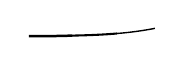
\begin{tikzpicture}\draw[line width=.9pt,line cap=butt] (0,0) .. controls (.18,0) and (.36,.002) .. (.55,.008);\draw[line width=.75pt,line cap=butt] (.55,.008) .. controls (.75,.012) and (.95,.02) .. (1.12,.035);\draw[line width=.5pt,line cap=butt] (1.12,.035) .. controls (1.31,.05) and (1.47,.075) .. (1.6,.1);\end{tikzpicture}}
Jusqu'à présent, on a maintenu $u$ fixe, on a fait varier $l$, resp. $(T/X,x,y)$. Si on regarde ce qui se passe pour $u\in\Gamma$ variable, les formules
\margin{76}

\scanpage{78}
essentielle triviale, qui fait \unsure{pendant|penser} \unsure{à|:} (6), est
\[
(2\unsure{8})\qquad {}^{uv}l={}^u({}^vl)
\qquad u,v\in\Gamma,\quad l:x\longrightarrow y
\quad\text{chemin dans }\unsure{\widehat{\Pi}_1(X)|\Pi_1(X)}
\]
\deleted{d'où,} si $l$ est chemin de $\Pi_1(X)$, d'où
\[
{}^vl=g_l(v)\cdot l
\]
\deleted{\unsure{grâce à} (6)} d'où on tire par (\unsure{6|8})
\[
{}^u({}^vl)={}^u\{g_l(v)\}\cdot \underset{\begin{gathered}
\rule{0.35pt}{3pt}\rule{2.2em}{0.35pt}\rule{0.35pt}{3pt}\\[-2pt]
g_l(u)\cdot l
\end{gathered}}{{}^ul}={}^ug_l(v)g_l(u)\cdot l
\]
d'où on tire
\[
(29)\qquad\left\{\begin{aligned}
{}^{\deleted{\unsure{u}}}g_l(uv)&={}^ug_l(v)\cdot g_l(u)\qquad\text{soit}\\
g_l^{-1}(uv)&=g_l^{-1}(u)\cdot{}^ug_l^{-1}(v)
\end{aligned}\right.
\]
Et de $=$
\[
(30)\qquad f_l(uv)=f_l(u)\cdot{}^uf_l(v)
\]
i.e. $f_{l\alpha}$ et $g_l^{-1}$ sont, pour $l$\unsure{.} fixé, $u$ variable, des $1$-cocycles \inserted{sur $\Gamma$} à valeurs dans $\widehat{\Pi}_1(X,x)$ resp. $\widehat{\Pi}_1(X,y)$, \unsure{\inserted{(groupes sur lesquels $\Gamma$ opère)}|(groupes sur lesquels $\Gamma$ opère)}, d'ailleurs déduits l'un de l'autre par l'isomorphisme
\diagram{\begin{tikzcd}[ampersand replacement=\&]
\widehat{\Pi}_1(X,x)
\arrow[r,phantom,"{\begin{gathered}\Pi_1(l)\\[-2pt]\unsure{\relbar\joinrel\relbar|\longrightarrow}\end{gathered}}"]
\&\widehat{\unsure{\Pi|\pi}}_1(X,y)
\end{tikzcd}}
induit par $l$ \deleted{\unsure{en $l$}} Ici, c'est la formule pour $f_l$ qui a une gueule plus sympathique que celle pour $g_l$ (pour (10)(11) c'était l'inverse --- \inserted{exprim.} ``multiplicativité en $l$''). Les $1$-cocycles obtenus (\deleted{\unsure{et}} $f$ \inserted{un $1$-cocycle} droit, $g$ un $1$-cocycle à gauche) correspondent à des $\Gamma$ torseurs à droite resp. à gauche sous $\widehat{\Pi}_1(X,x)$ resp! $\widehat{\unsure{\pi|\Pi}}_1(X,y)$, qui bien sûr n'est autre que $\operatorname{Hom}_{\widehat{\Pi}_1(X)}(x,y\unsure{)}$

\margin{On pourrait expliciter \unsure{un de vue qui voit le} couple $(f_l,g_l)$ comme un ``bicocycle'' sur $\Gamma$, relatif à un $\Gamma$-bitorseur $\operatorname{Hom}_{\widehat{\Pi}_1(X)}(x,y)$ sous $(\widehat{\Pi}_1(X,y),\widehat{\Pi}_1(X,x))$}
\margin{77}

